\documentclass[epj]{svjour}

\sloppy
\tolerance=3000
\emergencystretch=4em
\hbadness=10000
\hyphenpenalty=50

% Required packages
\usepackage{graphicx}
\usepackage{amsmath,amssymb,amsfonts}
\usepackage{mathtools}
\usepackage{booktabs}
\usepackage{multirow}
\usepackage{array}
\usepackage{enumitem}
\usepackage[dvipsnames,table]{xcolor}
\usepackage{hyperref}
\usepackage{bm}
\usepackage{microtype}
\usepackage{amsmath,amssymb}

\graphicspath{{figures/}}

\hypersetup{
    colorlinks=true,
    linkcolor=blue,
    citecolor=blue,
    urlcolor=blue
}

\begin{document}

\title{Schwarzschild Condensation: A QCD-Inspired Bose-Einstein Condensate Model for Non-Singular Black Hole Interiors and Cosmological Implications}

\author{Erdem Esa\thanks{\emph{Correspondence:} \href{mailto:erdem.esa.71@gmail.com}{erdem.esa.71@gmail.com}}}

\offprints{E. Esa}

\institute{Independent Researcher, Istanbul, Turkey}

\date{Received: \today\ / Revised version: \today}

\abstract{%
We propose a QCD-inspired phenomenological model---termed \emph{Schwarzschild Condensation} (SC)---in which the interior of a sufficiently compact gravitational object may be effectively described as undergoing a transition to a color-superconducting condensate, thereby providing a phenomenological regularization of the classical singular endpoint. At sufficiently high local densities associated with collapse inside a Schwarzschild-scale region, stellar matter may pass through electron capture, neutronization, and quark deconfinement. We construct the hadron--quark phase transition using a MIT bag plus CFL pairing equation of state, finding transition baryon densities $n_{\rm trans}/n_0 \simeq 1.8$--$2.0$ for fiducial parameters, in agreement with neutron-star core estimates. The Cooper-paired quarks may form a coherent condensate; the resulting interior is modelled as approximately de Sitter near the origin, yielding a regular effective interior with finite curvature invariants in the modeled domain. The Gross--Pitaevskii equation in this geometry reduces to a harmonic-trap problem admitting analytic Gaussian ground states. We test linear stability through a Cowling-approximation Bogoliubov--de Gennes spectral analysis. These ingredients are organized through a phase--spectral stability criterion linking dense-matter phase selection, finite curvature, positive fluctuation spectrum, and conditional ECO echo/ringdown signatures. We further add effective-core consistency diagnostics: an untapered energy-condition scan over 60 parameter sets, a tapered boundary-soft scan over 288 parameter sets, and curvature/compactness diagnostics over 96 metric-profile cases. We additionally solve static Einstein/TOV systems sourced by QCD-inspired CFL/bag effective equations of state, including an anisotropic effective-pressure extension, as matter-supported consistency checks rather than first-principles Einstein--QCD solutions. The tapered branch preserves regular-centre behaviour while suppressing the effective density and pressures at the matching surface, and the Ricci-scalar and Kretschmann-like proxies remain finite across the scanned regularized domain.
A kinetic analysis indicates that Cooper pairing is parametrically much faster than the gravitational collapse timescale ($\tau_{\rm pair}/t_{\rm ff} \sim 10^{-18}$), and the condensation criterion is not weakened, and may be reinforced, under rotation. When discussing gravitational-wave echoes we adopt the horizonless ultra-compact object interpretation, and derive quantitative ECO-channel estimates: for a GW150914-class merger ($60\,M_\odot$), the fundamental QNM frequency is $f_R \simeq 209$ Hz and the estimated echo delay is $\Delta t_{\rm echo} \simeq 8$ ms. A time-domain simulation of the assumed cavity dynamics reproduces the corresponding echo-train pattern within the adopted ECO setup. We provide a structured comparison with alternative non-singular black hole models and discuss limitations and falsifiable signatures throughout.
%
\PACS{
      {04.70.-s}{Physics of black holes} \and
      {04.70.Dy}{Quantum aspects of black holes, evaporation, thermodynamics} \and
      {12.38.Mh}{Quark-gluon plasma} \and
      {26.60.Kp}{Equations of state of neutron-star matter} \and
      {97.60.Lf}{Black holes}
     }
} %end of abstract

\maketitle

%============================================================
\section{Introduction}
\label{sec:intro}

Black holes are perhaps the most extreme objects in nature, residing at the interface between general relativity (GR) and quantum mechanics. Classical GR predicts that gravitational collapse inevitably terminates in a curvature singularity \cite{Penrose1965,HawkingEllis1973}, a prediction codified by the Penrose--Hawking singularity theorems under reasonable energy conditions. Yet the singularity itself signals the breakdown of classical theory: physical quantities diverge, predictability fails, and the smooth manifold structure is lost. Quantum mechanics, on the other hand, suggests that classical singular behavior lies outside the domain of applicability of the classical theory; even at the Planck scale, dimensional analysis indicates a finite characteristic density $\rho_P \approx 5.16 \times 10^{96}$ kg/m$^3$. The widespread expectation is therefore that the classical singularity should be replaced, in a successful quantum-gravitational description, by a regular structure of some kind \cite{Bardeen1968,Dymnikova1992,Hayward2006,BambiModesto2013}.

A complementary line of inquiry concerns the matter inside the black hole. Standard treatments often treat the interior matter content as an unspecified ``dust'' that collapses adiabatically. However, the matter compressed inside the Schwarzschild radius---comprising the original star's baryons, electrons, and any neutrinos produced during collapse---passes through a sequence of well-defined physical regimes: degenerate electron gas, neutronization, hadronic matter, quark deconfinement, and (potentially) color superconductivity. Each transition is governed by known nuclear and high-energy physics, and each occurs at a specific density threshold. The question we address in this paper is: \emph{what might be the final state of matter that is gravitationally compressed beyond the QCD deconfinement scale?}

\paragraph{Scope and interpretation.}
We adopt a phenomenological framework throughout: SC is presented as an effective, QCD-inspired model for regular compact-object interiors rather than as a derived theory. When discussing observational gravitational-wave echo signatures, we adopt the horizonless ultra-compact object (ECO) interpretation, in which a reflecting surface lies at $R_0 = R_s(1+\delta)$ for small $\delta > 0$; in this version no true event horizon is present. The regular interior solution constructed in Sect.~\ref{sec:interior} applies to both the genuine-horizon regular-black-hole and the ECO interpretation, but echoes are a feature only of the horizonless case.

\paragraph{Phase--spectral viewpoint.}
A useful way to organize the SC construction is to regard the interior as a
phase--spectral system. In this language, gravitational compression drives the matter sector across a dense-QCD threshold, the color-superconducting order parameter selects a new interior phase, and the perturbation spectrum determines whether that phase is dynamically stable. This viewpoint does not add a new microscopic assumption to the model; it only makes explicit the link between phase formation, regular geometry, spectral stability, and possible gravitational-wave observables.

Our central proposal is the following. When matter is compressed within a region of order $R_s = 2GM/c^2$, the configuration space available to each particle becomes so small that the system may be driven toward a coherent quantum state, in close analogy with the Bose-Einstein Condensation (BEC) of dilute cold atomic gases \cite{PethickSmith2008,Stringari2003,Dalfovo1999}. A crucial difference is that conventional BEC is driven by lowering the temperature so that the thermal de Broglie wavelength exceeds the interparticle spacing; \emph{Schwarzschild Condensation} is driven by gravitational compression that forces the relevant coherence length to exceed the local density-gradient scale of the core. Fermions cannot directly form a Bose condensate, but in the deconfined quark phase, Cooper pairing can produce composite bosons (diquarks) that may condense---a phenomenon known in QCD as color superconductivity \cite{Alford2008}.

The idea that black holes may be understood as condensates is not new. Dvali and Gomez proposed that black holes are graviton Bose condensates at a quantum critical point \cite{DvaliGomez2013}. Our approach is complementary: we begin from the matter sector and trace the phase transitions that stellar matter may undergo during gravitational collapse, arriving at an effective bosonic condensate through the established framework of color superconductivity. The two approaches need not be mutually exclusive.

A related line of inquiry concerns boson stars---self-gravitating configurations of scalar fields originally studied by Kaup \cite{Kaup1968} and Ruffini--Bonazzola \cite{Ruffini1969}, and extended to include self-interactions in many subsequent works (see \cite{LieblingPalenzuela2017} for a review). Boson stars share with SC the feature that a macroscopic quantum coherent state replaces a classical singularity, but they typically describe horizonless configurations of fundamental bosonic fields rather than condensates of composite particles formed during black hole collapse. The SC scenario can be viewed as a hybrid: in the regular-black-hole version, an event horizon exists and the interior is supported by a composite-boson condensate of Cooper-paired quarks; in the ECO version, the surface lies just outside the would-be horizon. Section~\ref{sec:comparison} provides a systematic comparison with these and other alternative models.

The structure of this paper is as follows. Section~\ref{sec:motivation} presents the physical motivation. Section~\ref{sec:density} compiles the elemental composition of stellar matter and computes the Schwarzschild density across the observed mass range. Section~\ref{sec:degeneracy} traces the sequence of fermionic phase transitions. Section~\ref{sec:condensation} introduces the SC hypothesis and the QCD-based phase transition criterion. Section~\ref{sec:kinetics} analyses the kinetic feasibility. Section~\ref{sec:interior} presents the regular interior solution. Section~\ref{sec:kerr} extends to rotating backgrounds. Section~\ref{sec:comparison} compares with alternative models. Section~\ref{sec:cosmology} draws cosmological analogies. Section~\ref{sec:information} addresses the information paradox. Section~\ref{sec:observations} presents observational predictions. Section~\ref{sec:limitations} acknowledges limitations, and Section~\ref{sec:conclusion} concludes.

%============================================================
\section{Physical Motivation}
\label{sec:motivation}

\subsection{The singularity problem}
\label{sec:singularity}

The Penrose--Hawking theorems \cite{Penrose1965,HawkingEllis1973} establish that under generic energy conditions, gravitational collapse forms a singularity within finite proper time. The Schwarzschild solution exhibits a curvature singularity at $r=0$ where the Kretschmann scalar diverges as $K = 48 G^2 M^2 / (c^4 r^6)$. This divergence is geometric: no observer-dependent coordinate choice can remove it. Yet the singularity violates every reasonable principle of physics---quantum mechanics forbids infinities, thermodynamics cannot accommodate states of zero volume and infinite energy density, and information theory requires that the dimension of the Hilbert space remain well-defined.

The natural resolution is that classical GR ceases to apply at scales where quantum effects of gravity become important---the Planck scale. However, this leaves open the question: \emph{what is the actual physical state of matter just below the singularity threshold}, in the regime where matter densities are extreme ($\sim 10^{19}$ kg/m$^3$ for stellar-mass black holes) but still far below Planck density ($\sim 10^{96}$ kg/m$^3$)? This is the regime governed not by quantum gravity but by QCD and quantum many-body physics, and it is the regime in which Schwarzschild Condensation may operate.

\subsection{The confinement--coherence argument}
\label{sec:confinement}

Consider a star of mass $M$ undergoing gravitational collapse to within its Schwarzschild radius $R_s = 2GM/c^2$. The mean number density of baryons is
\begin{equation}
n_B = \frac{\rho}{m_n} = \frac{M / [(4/3)\pi R_s^3]}{m_n} \propto M^{-2}.
\end{equation}
For a $1\,M_\odot$ black hole we obtain $n_B \approx 1.1 \times 10^{46}$ m$^{-3}$, corresponding to $\sim 70$ times nuclear saturation density. The mean interparticle spacing is
\begin{equation}
d = n_B^{-1/3} \approx 4.5 \times 10^{-16}\,\mathrm{m} = 0.45\,\mathrm{fm}.
\end{equation}
This interparticle spacing is comparable to the proton Compton wavelength $\lambda_C^{(p)} \approx 0.21$ fm, and---more importantly for our purposes---it is much smaller than the CFL coherence length $\xi_{\rm CFL} = \hbar c/(\pi\Delta) \sim 6$ fm for $\Delta \sim 10$ MeV (or $\sim 0.6$ fm for $\Delta \sim 100$ MeV). The relevant criterion for macroscopic coherence is not whether individual particles overlap, but whether the pair coherence length exceeds the density-gradient scale of the core: $\xi_{\rm CFL} \ll L_{\rm core}$. In the regime considered here, this condition is comfortably satisfied, justifying the use of a macroscopic order parameter description.

The physical inference is that order at the quantum level is plausibly enforced by gravitational confinement: any attempt to maintain distinguishable, classically localized degrees of freedom on length scales below $\xi_{\rm CFL}$ would require energy fluctuations incompatible with the stability of the underlying QCD condensate.

\subsection{Temperature- versus density-driven condensation}
\label{sec:temp_vs_density}

In conventional BEC, condensation occurs when the thermal de Broglie wavelength exceeds the interparticle spacing. In Schwarzschild Condensation, the trigger is fundamentally different: gravitational compression forces the relevant coherence length $\xi_{\rm CFL}$ to exceed the density-gradient scale of the core:
\begin{equation}
\xi_{\rm CFL} \ll L_{\rm core}.
\label{eq:SC_criterion}
\end{equation}
This is a temperature-independent condition. The condensate is not a thermal ground-state population, but a coherent macroscopic quantum state that may be enforced by spatial constraints, with the pairing physics provided by QCD at supranuclear densities.

\subsection{The role of fundamental constants}
\label{sec:constants}

The persistence of quantum order across vastly different scales---from atomic systems governed by the fine-structure constant $\alpha_{\rm em} \approx 1/137$ to nuclear systems governed by $\Lambda_{\rm QCD}$---suggests that order itself may be a universal feature of quantum matter, not a special property of any particular regime. We posit that this order may also persist in the extreme regime of gravitational compression to the Schwarzschild radius.

%============================================================
\section{Compositional and Density Analysis}
\label{sec:density}

\subsection{Solar composition as reference}
\label{sec:solar}

To establish concrete numbers, we begin with the mass fractions of the major elements composing the Sun, given in Table~\ref{tab:solar}. Hydrogen and helium together account for 98.3\% of solar mass, providing the dominant contribution to the baryon and electron counts. From these fractions one computes a total of $\sim 9.5 \times 10^{55}$ atoms and $\sim 1.0 \times 10^{56}$ electrons in the Sun.

\begin{table*}
\centering
\caption{Major elemental composition of the Sun (mass fractions).}
\label{tab:solar}
\begin{tabular}{lcc}
\hline\noalign{\smallskip}
Element & Symbol & Mass fraction \\
\noalign{\smallskip}\hline\noalign{\smallskip}
Hydrogen & H  & 73.46\% \\
Helium   & He & 24.85\% \\
Oxygen   & O  & 0.77\% \\
Carbon   & C  & 0.29\% \\
Iron     & Fe & 0.16\% \\
Neon     & Ne & 0.12\% \\
Others   & -- & 0.35\% \\
\noalign{\smallskip}\hline
\end{tabular}
\end{table*}

\subsection{Schwarzschild radius and mean density}
\label{sec:Rs_density}

For a black hole of mass $M$, the Schwarzschild radius is $R_s = 2GM/c^2$, and the mean density within this radius scales as
\begin{equation}
\bar\rho = \frac{3c^6}{32\pi G^3 M^2} \propto M^{-2}.
\label{eq:rho_avg}
\end{equation}
This $M^{-2}$ scaling is one of the most counterintuitive features of black hole physics: the more massive the black hole, the lower its mean density.

\subsection{Application to the observed mass range}
\label{sec:mass_range}

Table~\ref{tab:main_results} presents the key physical quantities at the Schwarzschild radius for a representative sequence of black holes spanning the full observed mass range. Figure~\ref{fig:mass_density} visualises this dependence.

\begin{table*}
\centering
\caption{Key physical quantities at the Schwarzschild radius for a representative sequence of black holes spanning the full observed mass range.}
\label{tab:main_results}
\begin{tabular}{lccccc}
\toprule
Object & $M$ [$M_\odot$] & $R_s$ [km] & $\bar\rho$ [kg/m$^3$] & $n_B/n_0$ & $\mu_q$ [MeV] \\
\midrule
Stellar BH (min) & 1 & 2.95 & $1.85\times10^{19}$ & $1.1\times10^4$ & 314.6 \\
Stellar BH (typical) & 10 & 29.5 & $1.85\times10^{17}$ & $1.1\times10^2$ & 314.6 \\
Stellar BH (max) & 100 & 295 & $1.85\times10^{15}$ & 1.1 & 314.6 \\
Sgr A$^*$ & $4.3\times10^6$ & $1.27\times10^7$ & $9.9\times10^5$ & $5.9\times10^{-7}$ & 313.0 \\
M87$^*$ & $6.5\times10^9$ & $1.92\times10^{10}$ & $4.4\times10^2$ & $2.6\times10^{-10}$ & 313.0 \\
Phoenix A & $1\times10^{11}$ & $2.95\times10^{11}$ & $1.9\times10^1$ & $1.1\times10^{-11}$ & 313.0 \\
\bottomrule
\end{tabular}
\end{table*}

We note that the quark chemical potential asymptotes to $\mu_q \to m_n c^2 / 3 \simeq 313$ MeV in the limit $M \to \infty$, corresponding to the free Fermi-gas limit where $p_F \to 0$ and $\mu_n \to m_n c^2$.

\begin{figure*}
\resizebox{0.95\textwidth}{!}{%
  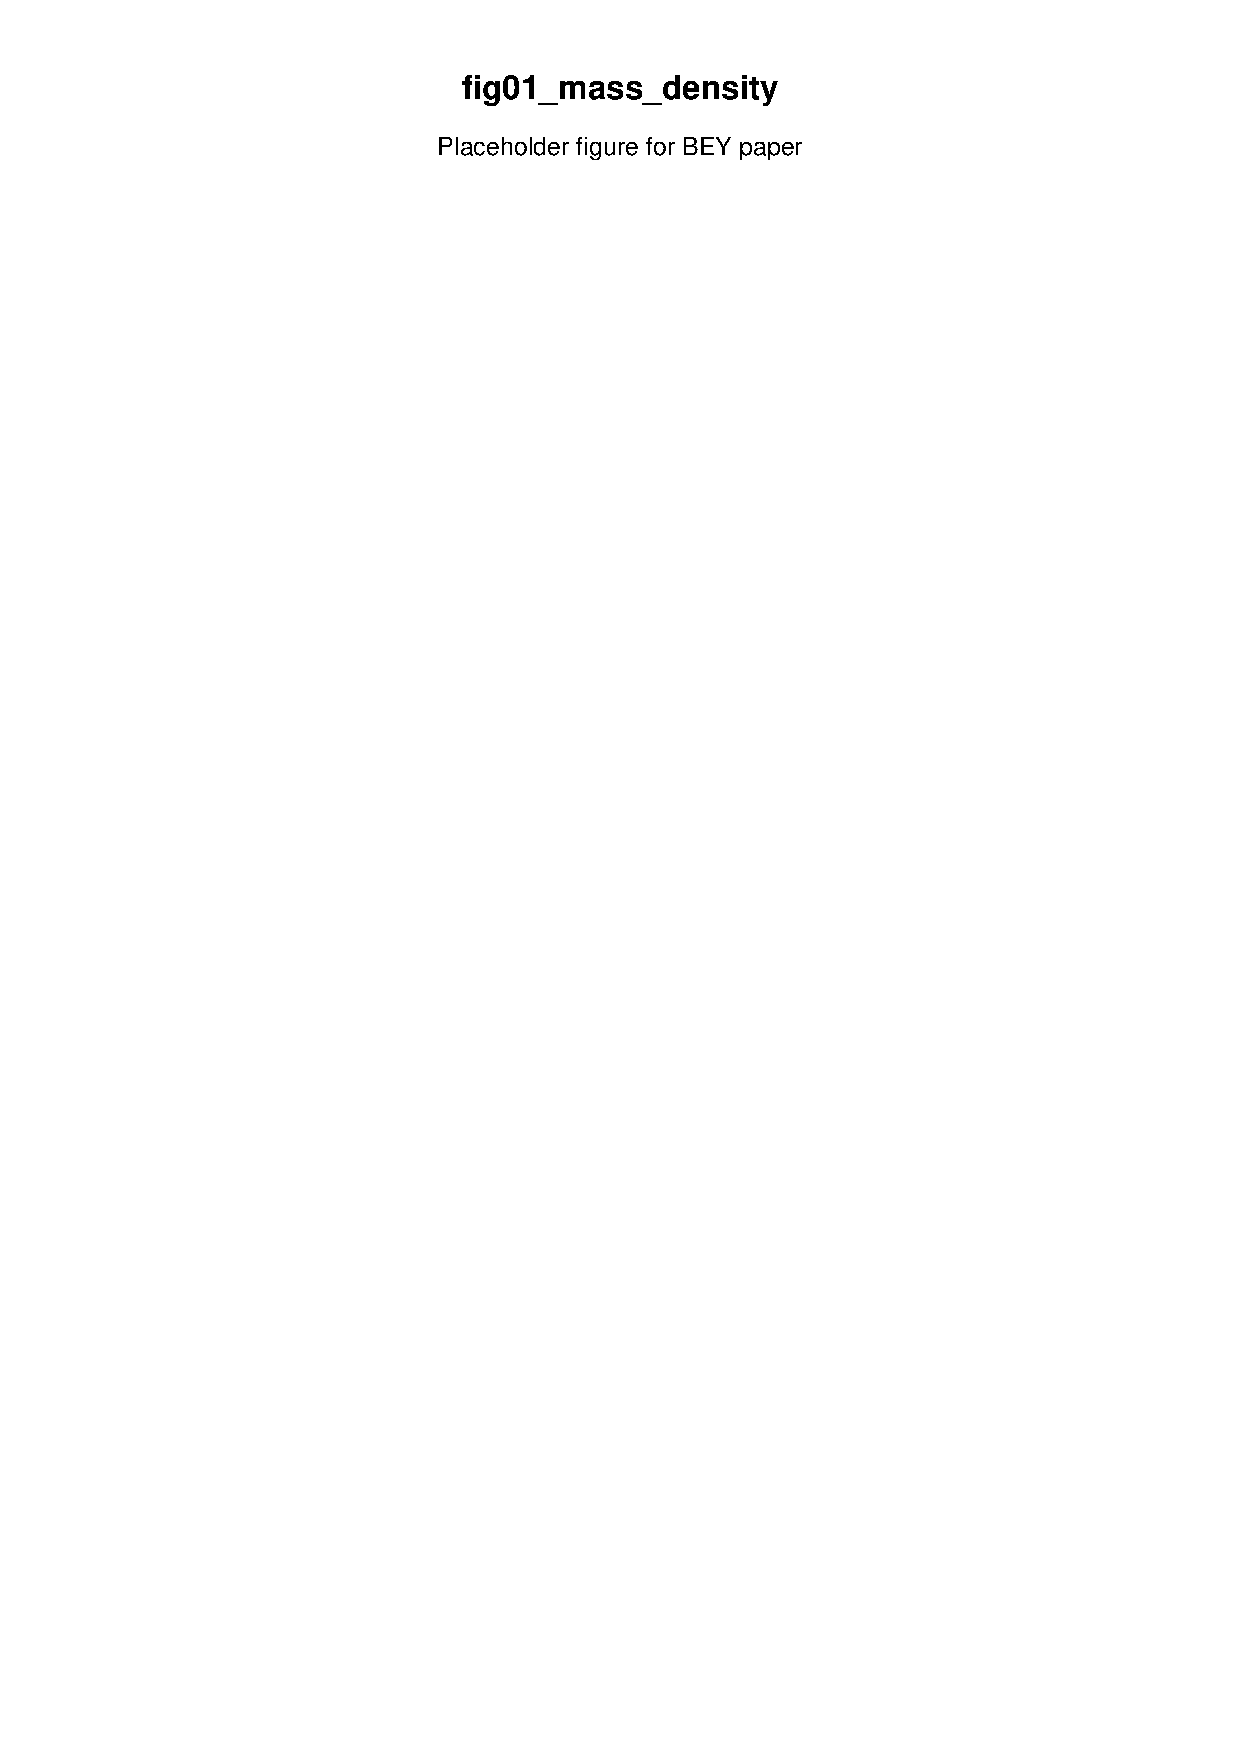
\includegraphics{fig01_mass_density.pdf}
}
\caption{Physical quantities at the Schwarzschild radius as a function of black hole mass, from $1\,M_\odot$ to Phoenix A ($\sim 10^{11}\,M_\odot$). Top-left: Schwarzschild radius. Top-right: mean density, with the nuclear saturation density $\rho_{\rm nuc} \approx 2.3 \times 10^{17}$ kg/m$^3$ shown for reference. Bottom-left: baryon number density in units of $n_0$. Bottom-right: quark chemical potential $\mu_q$ derived from the baryon Fermi momentum, with the QCD scale $\Lambda_{\rm QCD} \simeq 217$ MeV indicated.}
\label{fig:mass_density}
\end{figure*}

\subsection{Average versus local density: a resolution}
\label{sec:avg_local}

A critical observation is that no astrophysical black hole achieves Planck density as its \emph{average} density. Setting $\bar\rho = \rho_P$ in Eq.~\eqref{eq:rho_avg} yields $M \sim M_P \approx 2.18 \times 10^{-8}$ kg---a Planck-mass micro-black hole. We emphasise, however, that the average Schwarzschild density is used only as a scaling diagnostic. The actual phase transition criterion is local, depending on $\rho(r,t)$ and $\mu_B(r,t)$ during collapse. For stellar-mass collapse, local central densities are expected to plausibly enter the QCD regime; for supermassive objects, average-density arguments are insufficient and deconfinement depends on the collapse history and central density profile.

The relevant threshold is the QCD scale, $\mu_q \gtrsim \Lambda_{\rm QCD}$, which corresponds to local densities $\rho \sim 10^{17}$--$10^{18}$ kg/m$^3$. As Table~\ref{tab:main_results} and Fig.~\ref{fig:mass_density} show, this threshold appears to be exceeded by all observed black holes when measured by the relevant local quark chemical potential.

%============================================================
\section{Fermionic Degeneracy and Quark Deconfinement}
\label{sec:degeneracy}

\subsection{Electron capture and neutronization}
\label{sec:ecap}

The first phase transition during gravitational collapse beyond white-dwarf densities is electron capture: $e^- + p \to n + \nu_e$. This becomes energetically favourable when the electron Fermi energy exceeds $\sim 0.782$ MeV \cite{ShapiroTeukolsky1983}. The corresponding electron number density is $n_e \approx 1.5 \times 10^{36}$ m$^{-3}$, at mass density $\rho \approx 2.5 \times 10^9$ kg/m$^3$ \cite{LandauLifshitz1980}. Above this threshold, the matter rapidly neutronizes.

\subsection{Neutron instability and quark deconfinement}
\label{sec:deconf}

Beyond neutronization, neutrons themselves become unstable at sufficiently high density. The relativistic neutron chemical potential at Schwarzschild density (for a $1\,M_\odot$ black hole) is $\mu_n \approx 1.65$ GeV, exceeding the neutron rest mass by a factor of $\sim 1.8$. In this regime hadrons cannot remain confined; quarks become deconfined \cite{HaenselPotekhinYakovlev2007}.

The phase diagram in Fig.~\ref{fig:phase_diagram} shows that quark deconfinement may be achieved across the entire observed black hole mass range, with the simple chemical-potential estimate $\mu_q = \mu_n/3$ asymptoting to $\sim 313$ MeV. We emphasise, however, that this single-quantity estimate is only a scaling indicator; the proper deconfinement criterion is the thermodynamic comparison of hadronic and quark phase pressures, which we develop in Sect.~\ref{sec:qcd_transition}.

\begin{figure*}
\resizebox{0.95\textwidth}{!}{%
  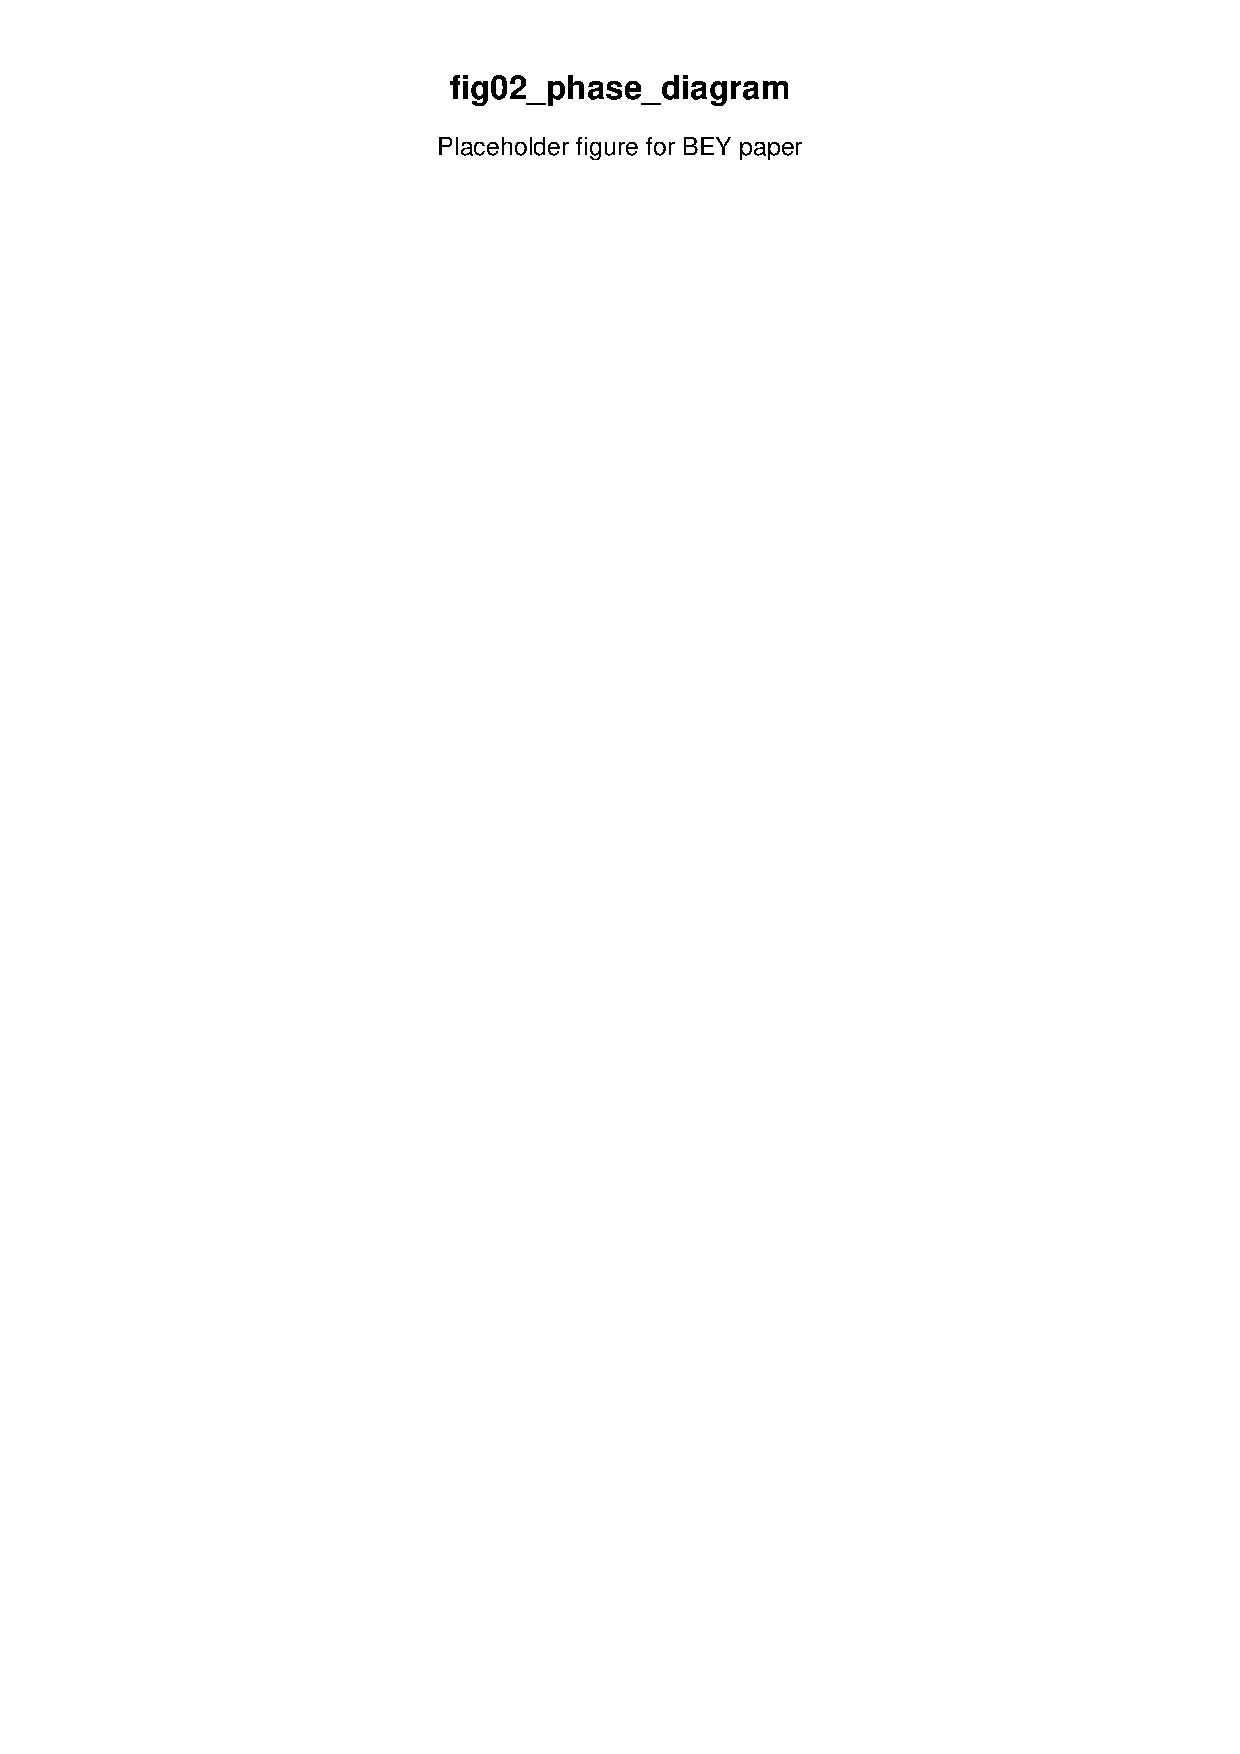
\includegraphics{fig02_phase_diagram.pdf}
}
\caption{Phase diagram of dense matter: quark chemical potential $\mu_q$ as a function of the mean density at the Schwarzschild radius. The solid blue curve is the relativistic Fermi-gas prediction. The dashed red line marks $\Lambda_{\rm QCD} = 217$ MeV; the green shaded region is the deconfinement domain. Vertical lines indicate representative black holes.}
\label{fig:phase_diagram}
\end{figure*}

\subsection{Fermi temperature and degeneracy parameter}
\label{sec:fermi_temp}

The Fermi temperature for baryons at Schwarzschild density (for $M = 1\,M_\odot$) is $T_F \approx 8.3 \times 10^{12}$ K. For any plausible quasi-equilibrium internal temperature $T \ll T_F$, the matter is deeply degenerate. We discuss the validity of this assumption in Sect.~\ref{sec:limitations}.

%============================================================
\section{The Schwarzschild Condensation Hypothesis}
\label{sec:condensation}

\subsection{Statement of the hypothesis}
\label{sec:hypothesis}

We now formulate the central hypothesis of this paper.

\begin{quote}
\textbf{Schwarzschild Condensation Hypothesis.}
We propose that, given the extreme densities reached during gravitational collapse to within the Schwarzschild radius and the corresponding deconfinement of quark matter, a configuration consistent with Cooper-paired quark Bose-Einstein condensation may be a candidate endpoint. Whether such a configuration is actually reached on the timescale of gravitational collapse is analysed in Sect.~\ref{sec:kinetics}. If reached, this condensate would replace the classical singular endpoint, within the effective description, by a regular coherent quantum core of finite energy density. We treat this hypothesis as a phenomenological scenario to be tested by its internal consistency (Sects.~\ref{sec:interior}--\ref{sec:kerr}) and observational predictions (Sect.~\ref{sec:observations}).
\end{quote}


The logical structure of the Schwarzschild Condensation scenario is summarized
schematically in Fig.~\ref{fig:bey_collapse_to_condensate_chain}. The figure
should be read as a conditional mechanism chain: gravitational compression may
drive matter into a deconfined quark regime, CFL-like pairing may generate
effective bosonic Cooper pairs, and the resulting condensate may support a
regular finite-density interior. The possible echo channel belongs only to the
horizonless ECO interpretation and is not required by the regular-interior
construction itself.

\begin{figure*}[t!]
\centering
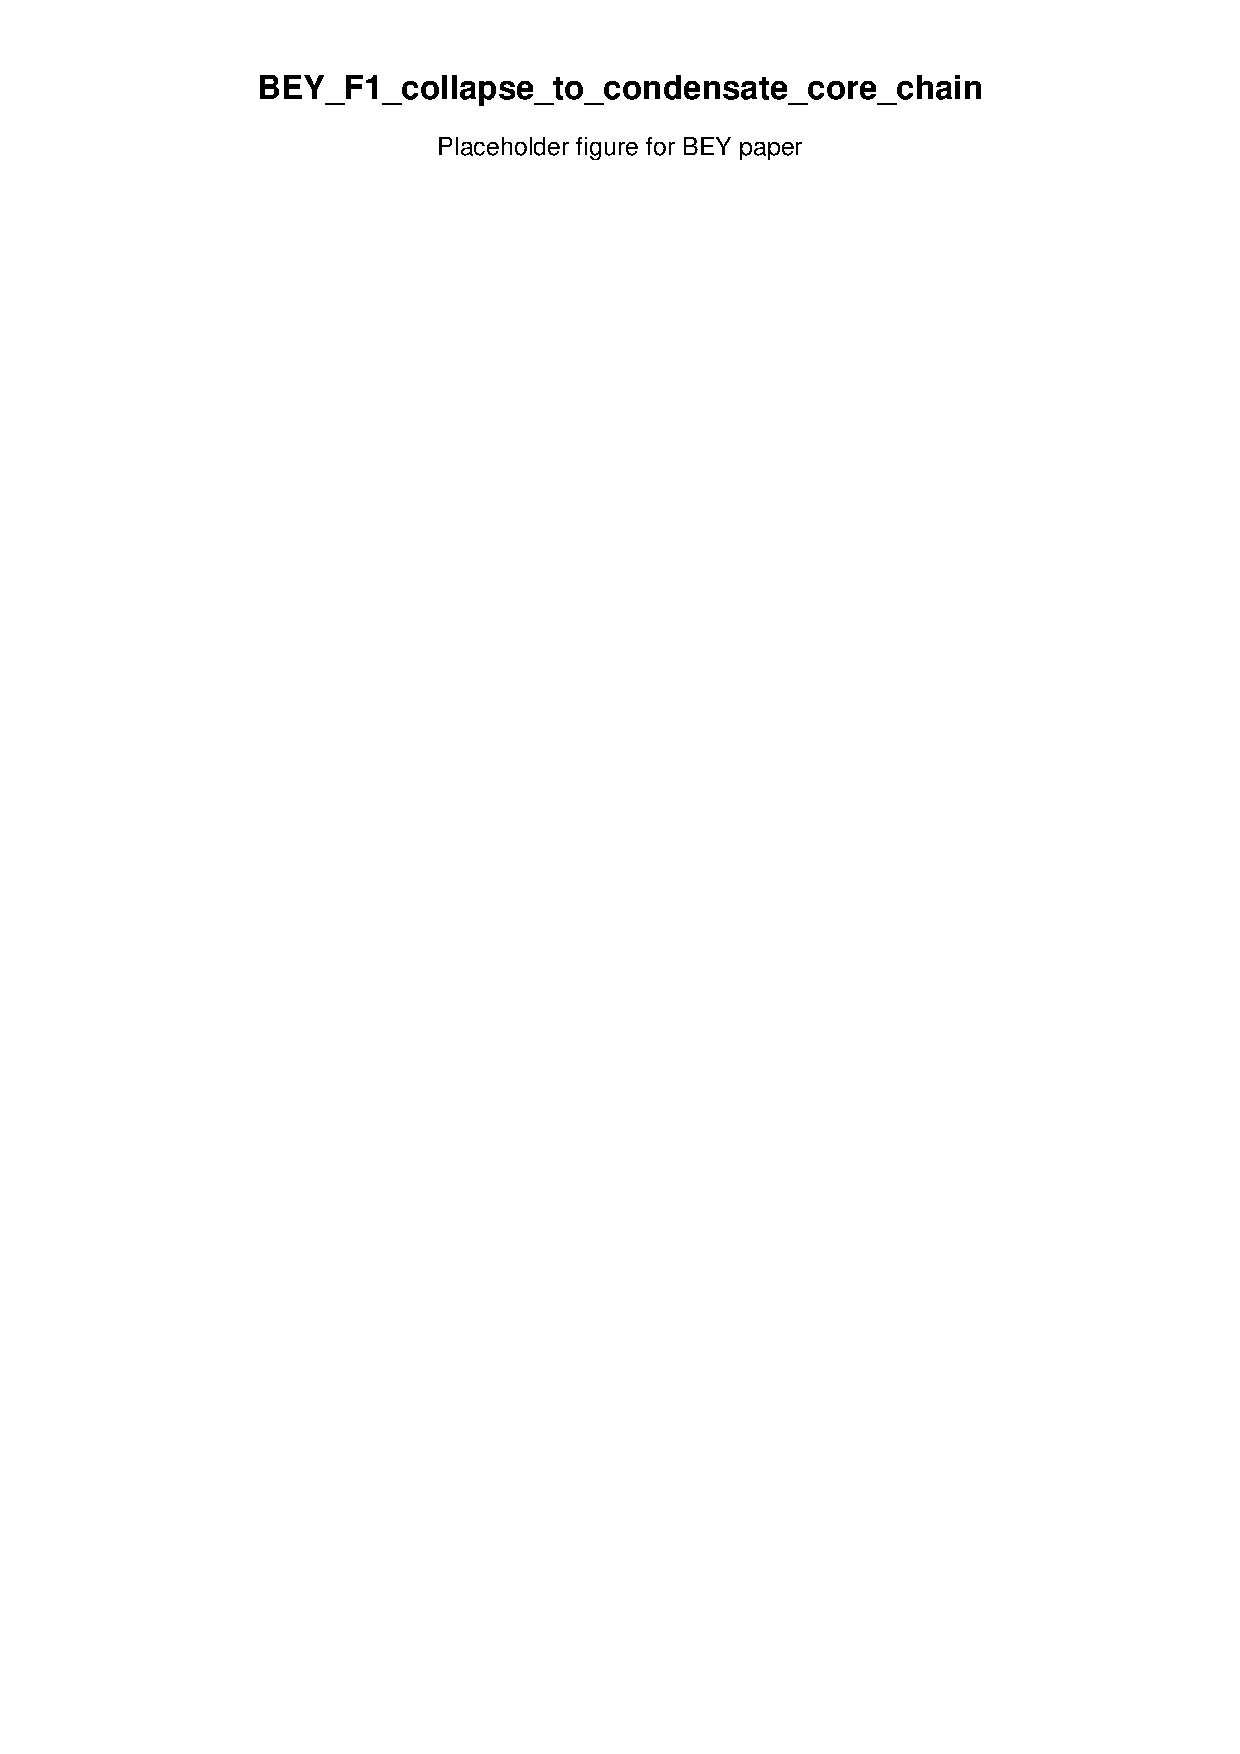
\includegraphics[
width=0.96\textwidth,
height=0.38\textheight,
keepaspectratio
]{figures/BEY_F1_collapse_to_condensate_core_chain.pdf}
\caption{
Mechanism chain of the Schwarzschild Condensation scenario. Gravitational
compression may push matter into a regime where quark deconfinement becomes
relevant. In the QCD-inspired effective description, CFL-like pairing then
allows fermionic quark matter to form effective bosonic Cooper pairs. If a
coherent condensate is reached, the central region is modeled as a regular
finite-density core rather than a classical curvature singularity. The final
echo channel is conditional: it applies only in the horizonless ECO
interpretation and is not required by the regular-interior construction.
}
\label{fig:bey_collapse_to_condensate_chain}
\end{figure*}

\subsection{QCD phase transition: MIT bag plus CFL pairing}
\label{sec:qcd_transition}

To establish whether quark matter is actually thermodynamically favoured at the relevant densities, we construct the hadron--quark phase transition using a standard MIT bag model with CFL pairing corrections \cite{Alford2008}. The grand potential of the CFL quark phase at zero temperature is
\begin{equation}
\Omega_{\rm CFL}(\mu_q) = -\frac{3 a_4}{4\pi^2}\mu_q^4 + \frac{3 m_s^2}{4\pi^2}\mu_q^2 - \frac{3\Delta^2}{\pi^2}\mu_q^2 + B,
\label{eq:Omega_CFL}
\end{equation}
where $\mu_q = \mu_B/3$ is the quark chemical potential, $a_4 \approx 0.7$ is the perturbative QCD correction, $m_s$ is the strange quark mass, $\Delta$ is the CFL pairing gap, and $B$ is the bag constant. The hadronic phase is described as a free neutron gas to first approximation.

The transition occurs where $P_{\rm hadronic}(\mu_B) = P_{\rm quark}(\mu_B)$. We performed a parameter scan over $B^{1/4} \in [145, 180]$ MeV, $\Delta \in [10, 100]$ MeV, and $m_s \in [95, 150]$ MeV. Results for the fiducial case ($B^{1/4} = 145$ MeV, $\Delta = 10$ MeV, $m_s = 95$ MeV) give:
\begin{align}
\mu_{B,{\rm trans}} &\simeq 942\,\mathrm{MeV}, \\
n_{B,{\rm trans}}/n_0 &\simeq 1.79,
\end{align}
i.e., the transition occurs at about twice nuclear saturation density---squarely within the neutron-star core density range (Fig.~\ref{fig:qcd_phase}). Out of 27 parameter combinations, 8 admit a clean first-order transition; the remainder correspond to parameter regions where CFL is dominant at all densities above saturation.

\begin{figure*}
\resizebox{0.92\textwidth}{!}{%
  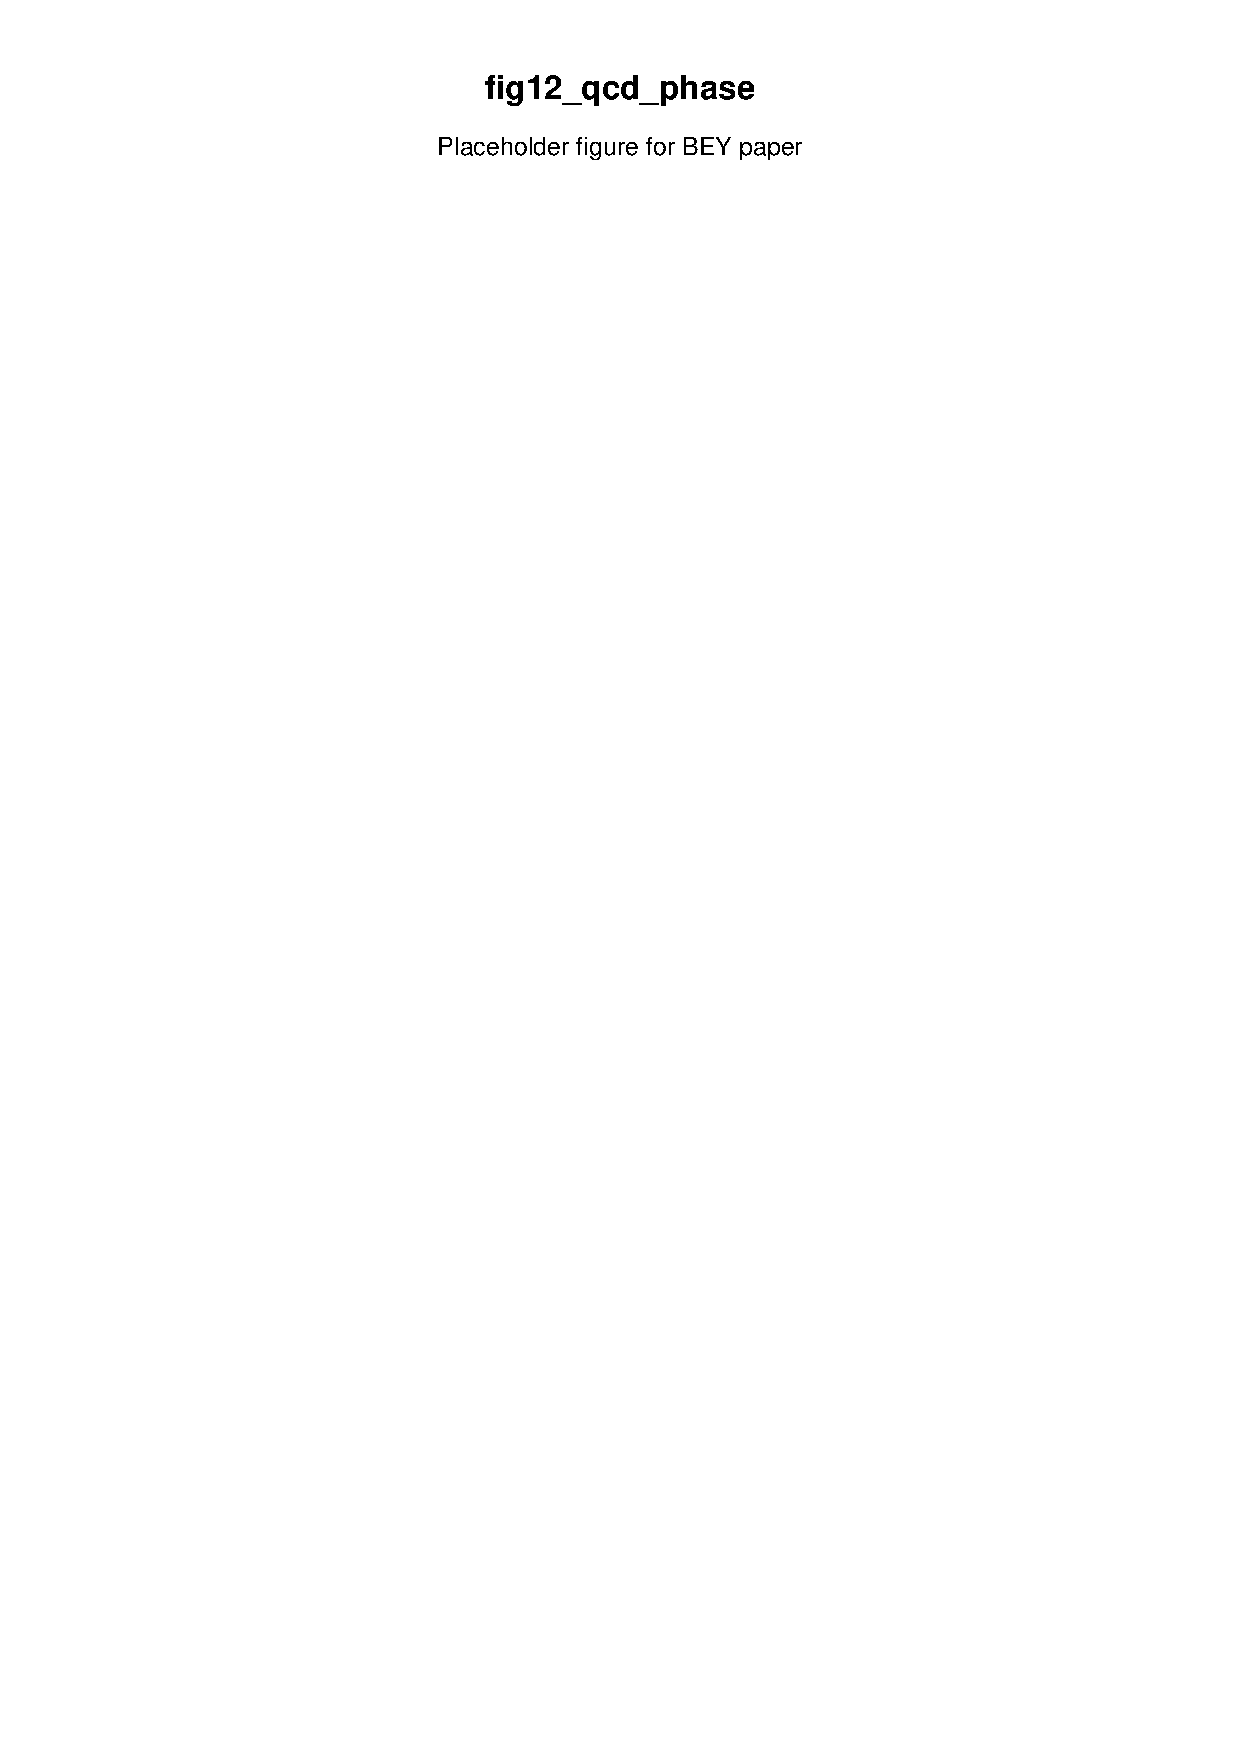
\includegraphics{fig12_qcd_phase.pdf}
}
\caption{QCD phase transition: hadronic to color-flavor-locked quark matter from a MIT bag plus CFL pairing analysis. \textbf{Left:} transition density $n_{\rm trans}/n_0$ as a function of the bag constant $B^{1/4}$ for three values of the CFL pairing gap $\Delta$. The fiducial point ($B^{1/4} = 145$ MeV, $\Delta = 10$ MeV) is marked. The grey band shows the neutron-star core density range, $n \sim 2$--$6\,n_0$. \textbf{Right:} transition density as a function of the CFL gap $\Delta$ at fixed $B^{1/4} = 145$ MeV.}
\label{fig:qcd_phase}
\end{figure*}

The key conclusion is that under standard QCD parameter choices, hadronic matter transitions to a CFL quark-matter phase at densities accessible during gravitational collapse, consistent with neutron-star and quark-star modelling \cite{Alford2008,Glendenning1996}.

\subsection{Condensation criterion}
\label{sec:condensation_criterion}

The CFL coherence length $\xi_{\rm CFL} = \hbar c/(\pi\Delta)$ sets the scale over which the order parameter is coherent. For $\Delta = 10$--$100$ MeV, $\xi_{\rm CFL} \sim 0.6$--$6$ fm. Condensation describes a macroscopic order parameter wherever this coherence length is much smaller than the density-gradient scale of the core, $\xi_{\rm CFL} \ll L_{\rm core}$. In typical interior regions with $L_{\rm core} \gtrsim$ km, this condition is comfortably satisfied.

\paragraph{Cooper pair effective mass and parameter sensitivity.}
We use $m_{\rm pair} \sim 10$ MeV/$c^2$ as the effective mass of the composite scalar order parameter, set by the lower edge of the CFL pairing gap range $\Delta \sim 10$--100 MeV \cite{Alford2008}. The characteristic core width $\sigma = \sqrt{\hbar/(m_{\rm pair}\omega)}$ scales as $\sigma \propto m_{\rm pair}^{-1/2}$, so varying $m_{\rm pair}$ within the plausible range changes $\sigma$ by a factor of $\sim 3$. Table~\ref{tab:sensitivity} shows the core sizes for a $1\,M_\odot$ black hole.

\begin{table*}
\centering
\caption{Sensitivity of SC core size $\sigma$ to the assumed Cooper-pair effective mass for $M = 1\,M_\odot$.}
\label{tab:sensitivity}
\begin{tabular}{cc}
\hline\noalign{\smallskip}
$m_{\rm pair}$ [MeV/$c^2$] & $\sigma$ [m] \\
\noalign{\smallskip}\hline\noalign{\smallskip}
10  & $7.6 \times 10^{-6}$ \\
30  & $4.4 \times 10^{-6}$ \\
100 & $2.4 \times 10^{-6}$ \\
\noalign{\smallskip}\hline
\end{tabular}
\end{table*}

\subsection{Color superconductivity: the fermion-boson bridge}
\label{sec:CFL_bridge}

Fermions cannot directly form a Bose-Einstein condensate. The resolution comes from QCD itself: at high baryon densities $\mu_q \gg \Lambda_{\rm QCD}$, quarks near the Fermi surface experience an attractive interaction in the color-antitriplet channel via single-gluon exchange, leading to Cooper pairing of the BCS type \cite{Alford2008}. The pair condensate
\begin{equation}
\langle q^a_\alpha q^b_\beta \rangle \neq 0
\end{equation}
breaks $SU(3)_c \times U(1)_B$ down to a residual symmetry. In the Color-Flavor-Locked (CFL) phase, all three colors and three light flavors participate symmetrically, with pairing gap $\Delta \sim 10$--100 MeV. The Cooper pairs are composite bosons with integer spin and can undergo Bose-Einstein condensation. Analogous mechanisms operate in superfluid $^3$He and in electronic superconductors.

\subsection{Effective Lagrangian and QCD calibration}
\label{sec:lagrangian}

The macroscopic long-wavelength dynamics of the Cooper-paired quark condensate in the gravitational background may be described by an effective relativistic Lagrangian of the form
\begin{equation}
\mathcal{L}_{\rm SC} = \sqrt{-g}\left[
g^{\mu\nu}(\partial_\mu \Psi^\dagger)(\partial_\nu \Psi) 
- m_{\rm pair}^2 c^2 |\Psi|^2 
- \tfrac{1}{2} g_{\rm int} |\Psi|^4
\right],
\label{eq:Lagrangian}
\end{equation}
where $\Psi$ is the complex scalar order parameter, $m_{\rm pair}$ is the Cooper-pair mass, and $g_{\rm int}$ is the effective $|\Psi|^4$ self-coupling.

\paragraph{QCD calibration of the self-interaction.}
The dimensionless self-coupling $\tilde{g}$ used in our self-consistent calculations (Sect.~\ref{sec:self_consistent}) is not a free parameter but is set by underlying QCD physics. In the CFL phase, the relevant four-quark interaction strength scales as $g_{\rm int} \sim \Delta^2 / n_0^{1/3}$ \cite{Alford2008}, giving dimensionless values $\tilde{g} \sim 0.05$--$0.5$ for $\Delta \sim 10$--$100$ MeV, bracketing our fiducial choice $\tilde{g} = 0.1$.

\subsection{GP-like effective equation in curved spacetime}
\label{sec:GP_equation}

The dynamics of the condensate order parameter $\Psi$ in the curved interior spacetime may be described by a Gross-Pitaevskii-like effective equation, treated as a phenomenological long-wavelength description of the CFL order parameter rather than a fundamental dynamical equation. For the static configurations relevant here, the equation reduces to a stationary form which we solve explicitly in Sect.~\ref{sec:harmonic} (analytic Gaussian) and Sect.~\ref{sec:self_consistent} (self-consistent BVP).

%============================================================
\section{Kinetic Feasibility: Condensation versus Collapse}
\label{sec:kinetics}

A central physical question for any candidate non-singular black-hole interior is whether the proposed configuration can actually form on the timescale of gravitational collapse, or whether kinetic bottlenecks prevent it.

\paragraph{Free-fall timescale.}
The characteristic gravitational timescale for compression to the Schwarzschild radius is $t_{\rm ff} \simeq \sqrt{R_s^3/(GM)} = (2GM/c^3)\sqrt{2}$, yielding $t_{\rm ff}(1\,M_\odot) \approx 1.4 \times 10^{-5}$ s.

\paragraph{Cooper-pair formation timescale.}
In the CFL phase, the characteristic time for Cooper-pair formation is set by the pairing gap: $\tau_{\rm pair} \simeq \hbar/\Delta_{\rm CFL}$. For $\Delta_{\rm CFL} \sim 50$ MeV, this gives $\tau_{\rm pair} \approx 1.3 \times 10^{-23}$ s---a microscopic QCD timescale.

\paragraph{Hierarchy of timescales.}
The ratio
\begin{equation}
\frac{\tau_{\rm pair}}{t_{\rm ff}} \approx 9 \times 10^{-19}\quad (M = 1\,M_\odot)
\end{equation}
shows that Cooper pairing is faster than gravitational collapse by approximately \emph{eighteen orders of magnitude}. This ratio scales as $\tau_{\rm pair}/t_{\rm ff} \propto M^{-1}$, so it becomes even more favourable for more massive black holes (Fig.~\ref{fig:timescales}). The kinetic conclusion is that \emph{Cooper pairing is parametrically much faster than the gravitational-collapse timescale}, and the SC configuration is not kinematically obstructed.

\begin{figure*}
\resizebox{0.92\textwidth}{!}{%
  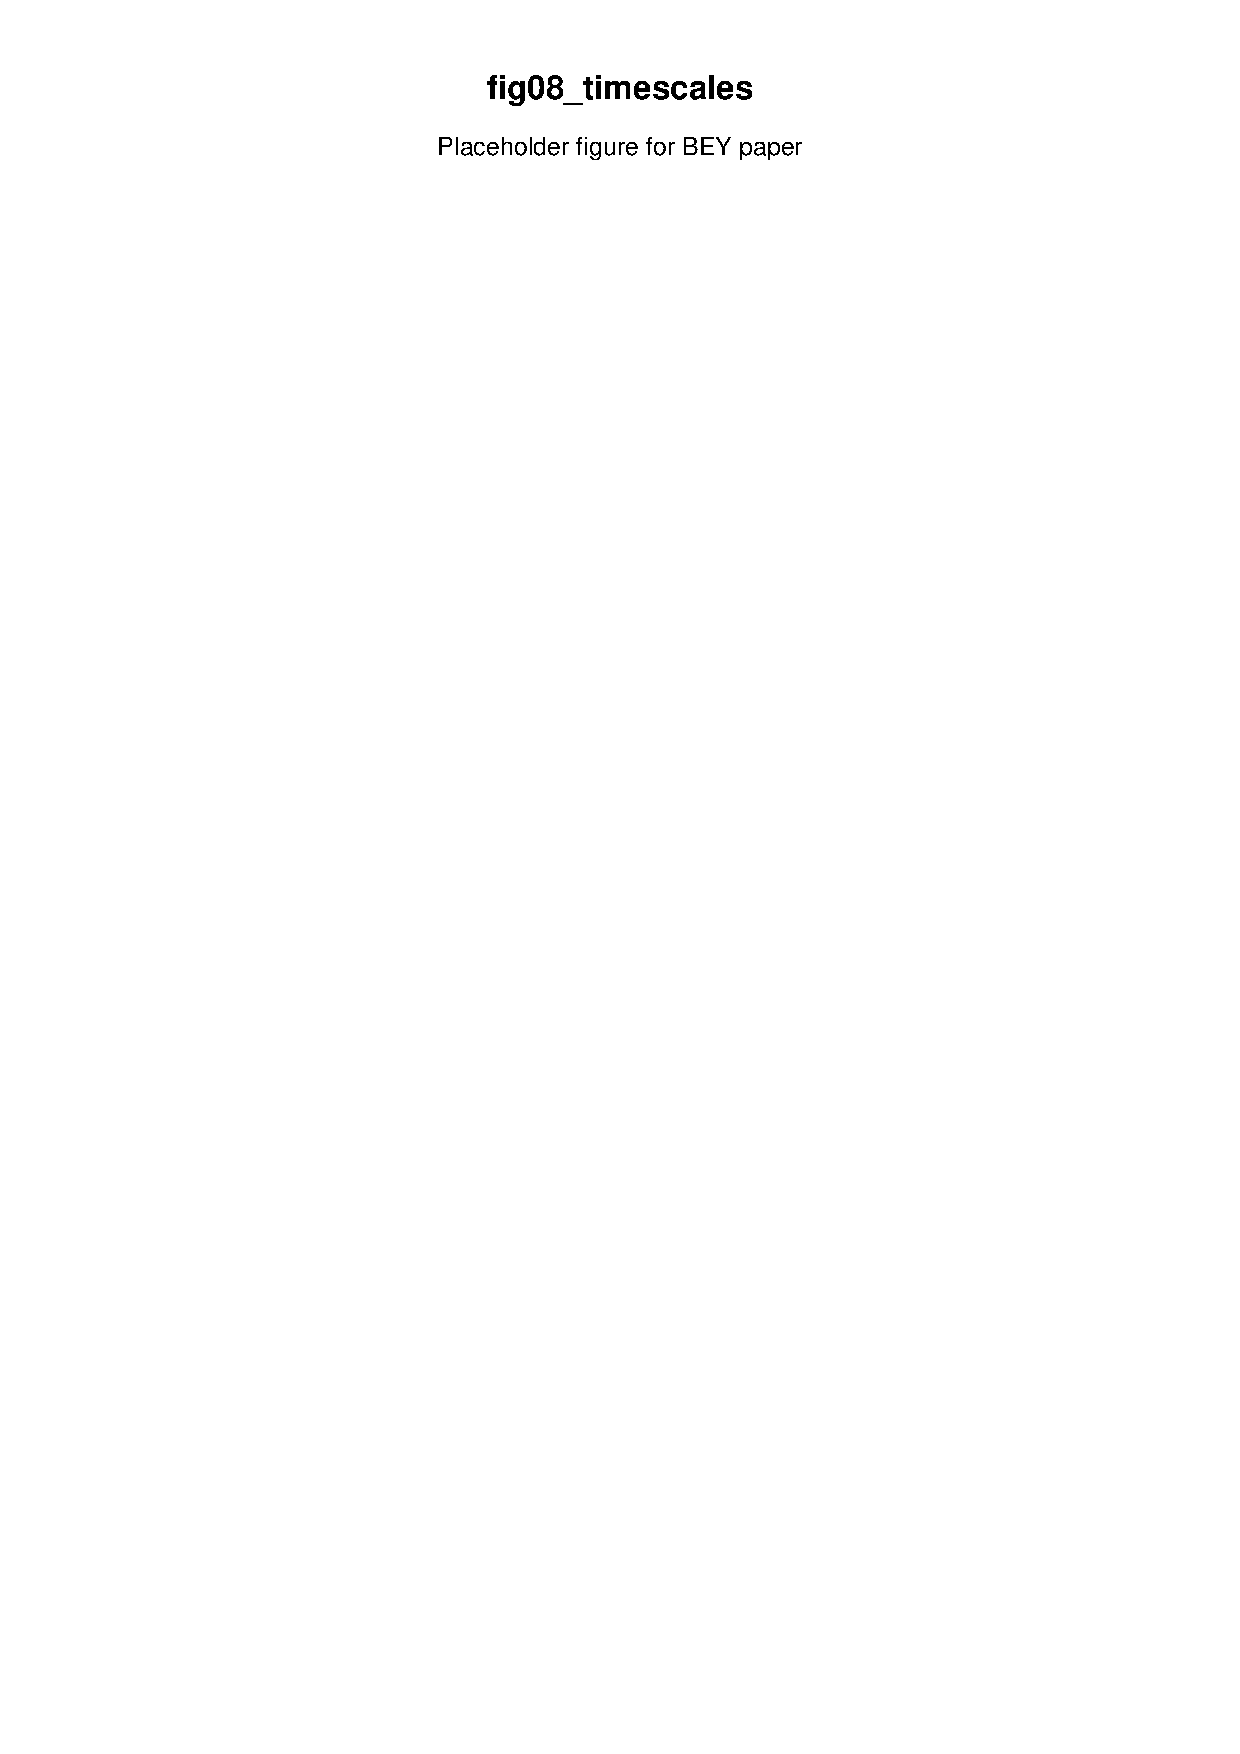
\includegraphics{fig08_timescales.pdf}
}
\caption{Characteristic timescales relevant to Schwarzschild Condensation. \textbf{Left:} the gravitational free-fall time $t_{\rm ff}$, the characteristic trap period $1/\omega$, and the Cooper-pair formation time $\tau_{\rm pair} = \hbar/\Delta_{\rm CFL}$ (mass-independent). \textbf{Right:} The ratio $\tau_{\rm pair}/t_{\rm ff} \lesssim 10^{-18}$ across the full astrophysical mass range indicates that Cooper pairing is parametrically fast on the relevant gravitational timescale.}
\label{fig:timescales}
\end{figure*}

This result addresses one of the most frequently raised objections to BEC-like models of black-hole interiors: the formation timescale is set by microscopic QCD physics, while the relevant gravitational timescale is set by macroscopic geometry. The vast disparity between these scales ($\sim 18$--$30$ orders of magnitude depending on mass) means that a substantial kinetic suppression factor would be required to obstruct condensation within the adopted estimates.

%============================================================
\section{Non-Singular Compact-Object Interior}
\label{sec:interior}

\subsection{Approximately de Sitter core}
\label{sec:approx_dS}

The interior of the SC core is modelled as filled with a smooth, finite-density condensate. For any condensate density profile $\rho(r)$ that is finite and smooth at $r=0$, we have $\rho(r) = \rho_0 + \mathcal{O}(r^2)$ near the origin. The enclosed mass therefore satisfies
\begin{equation}
m(r) = 4\pi\int_0^r \rho(r')\,r'^2\,dr' = \frac{4\pi}{3}\rho_0 r^3 + \mathcal{O}(r^5),
\end{equation}
and the metric function is
\begin{equation}
f(r) = 1 - \frac{2Gm(r)}{c^2 r} = 1 - \frac{8\pi G \rho_0}{3 c^2}\,r^2 + \mathcal{O}(r^4).
\label{eq:approx_dS}
\end{equation}
This is precisely the de Sitter form near the origin, with effective curvature length $\ell^2 = 3c^4/(8\pi G \rho_0 c^2)$. Crucially, this approximation does not require the interior density to be exactly constant throughout: any smooth condensate profile that is finite at $r=0$ produces an approximately de Sitter behaviour near the centre, and therefore a regular geometry.

The Kretschmann scalar of the approximately de Sitter region is
\begin{equation}
K^{\rm (in)} \simeq \frac{8}{3}\Lambda^2 = \frac{24}{\ell^4},
\end{equation}
finite at $r=0$. Within the effective interior metric, the curvature singularity is absent: this is the central geometric fact that motivates the SC framework. Figure~\ref{fig:desitter_core} compares the metric and Kretschmann scalar in the matched interior-exterior geometry.

\begin{figure*}
\resizebox{0.92\textwidth}{!}{%
  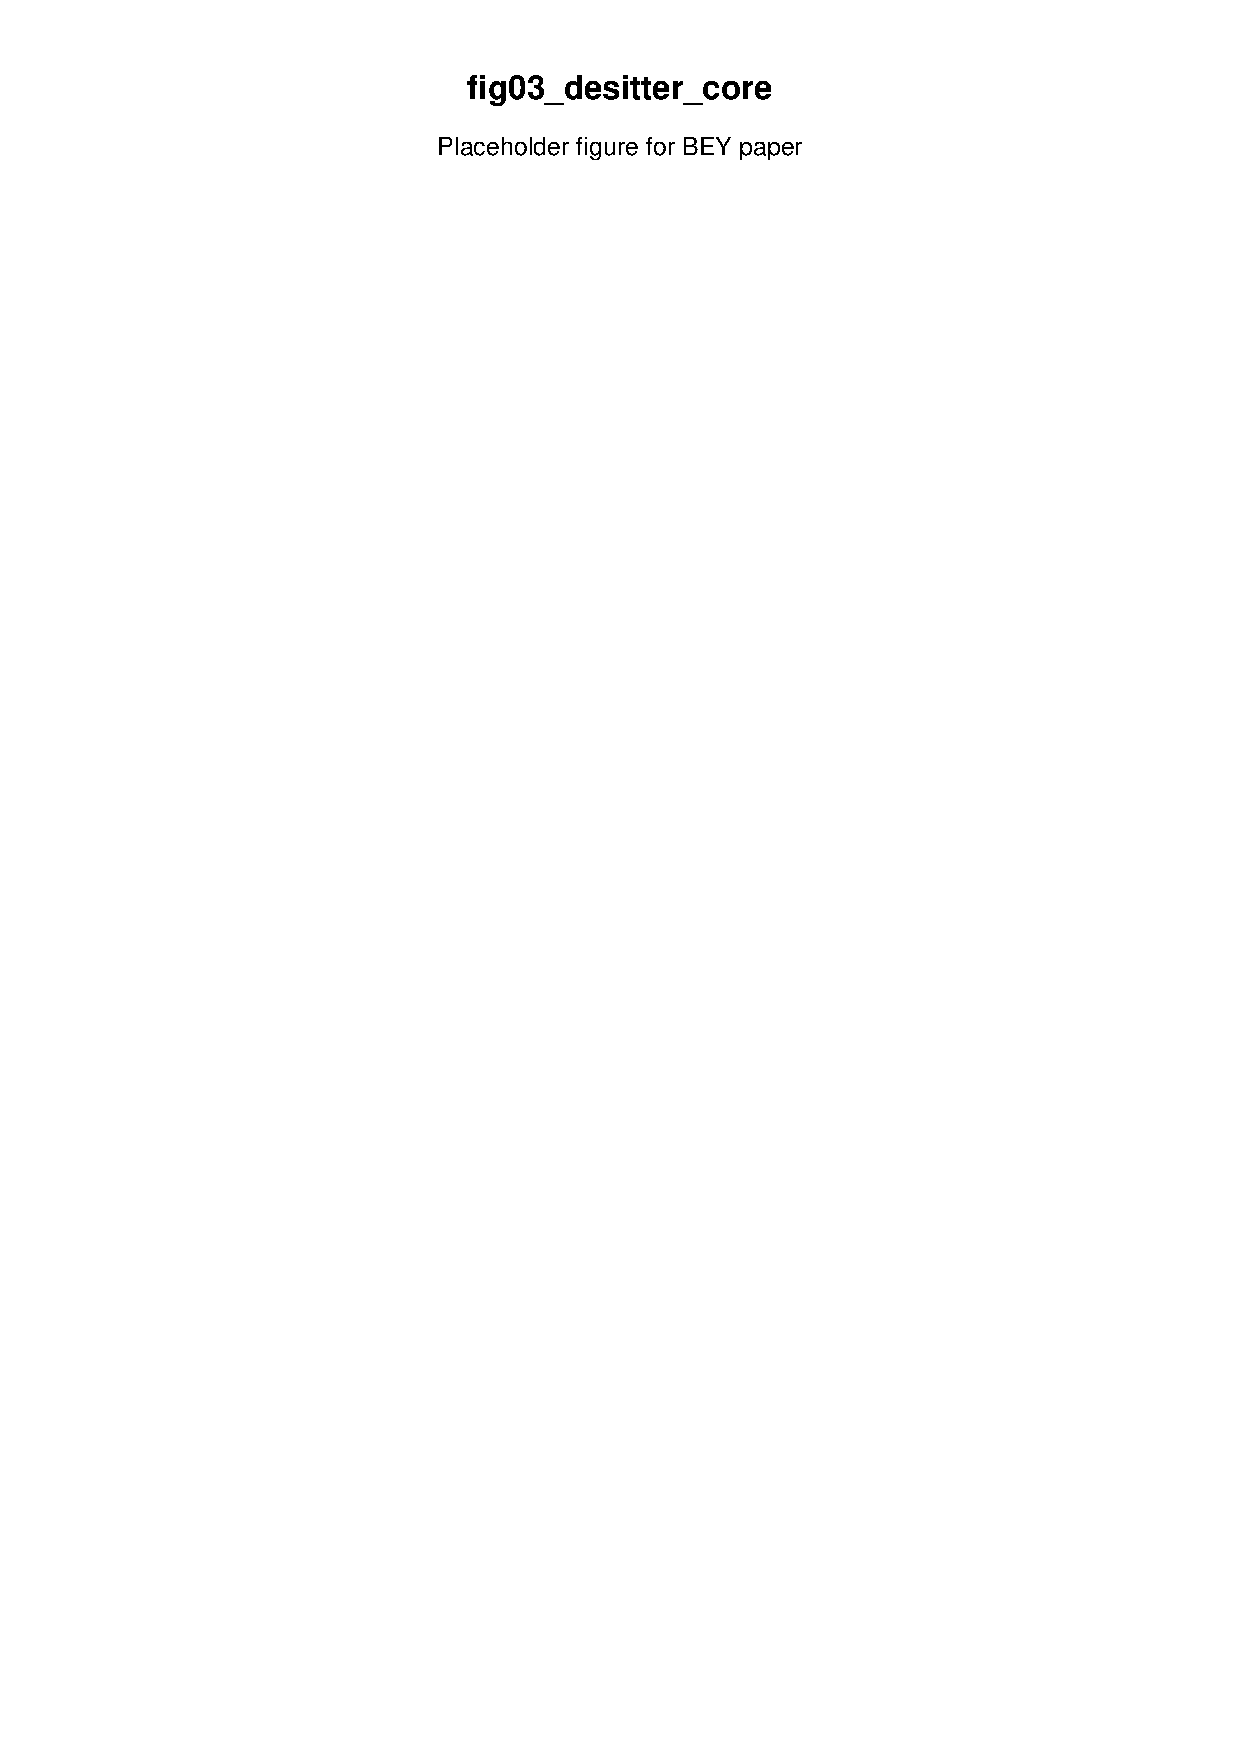
\includegraphics{fig03_desitter_core.pdf}
}
\caption{Left: Metric components $-g_{tt}$ and $g_{rr}$ for the matched approximately de Sitter interior and Schwarzschild exterior, plotted versus $r/R_s$. The interior is regular at $r=0$. Right: The Kretschmann scalar $K \cdot \ell^4$. In the interior, $K \simeq (8/3)\Lambda^2$ is approximately constant; the would-be exterior $r^{-6}$ divergence at $r=0$ is regularised.}
\label{fig:desitter_core}
\end{figure*}

\subsection{Israel junction conditions and shell dynamics}
\label{sec:junction}

In the ECO interpretation, the interior and exterior metrics are matched at the surface $r = R_0 = R_s(1+\delta)$ using the Israel junction conditions \cite{Israel1966}. Continuity of the induced metric and the Lanczos equation give the surface energy-momentum tensor
\begin{equation}
S_{ab} = -\frac{1}{8\pi G}\left([K_{ab}] - h_{ab}[K]\right) = \mathrm{diag}(-\sigma_{\rm sh}, p_{\rm sh}, p_{\rm sh}).
\end{equation}
The shell surface density $\sigma_{\rm sh}$ and tangential pressure $p_{\rm sh}$ depend on $M$, $R_0$, and the interior density. The dominant energy condition $\sigma_{\rm sh} \geq |p_{\rm sh}|$ is satisfied for SC matching parameters consistent with the stable gravastar regime \cite{MazurMottola2004,Visser2004}. We note that for the limiting case $R_0 = 2M$ exactly, the surface is null and the standard timelike Israel formalism requires modification; we restrict our analysis to $\delta > 0$.

The stability of the matching surface against radial perturbations follows from the gravastar literature \cite{MazurMottola2004,Visser2004}: the analogous de Sitter--Schwarzschild matching is dynamically stable provided the surface equation of state satisfies appropriate causality conditions ($v_s^2 = dp_{\rm sh}/d\sigma_{\rm sh} \leq c^2$, typically realised by a stiff fluid $p_{\rm sh} = w\sigma_{\rm sh}$ with $0 < w \leq 1$). We adopt these conclusions for the SC matching layer.

\subsection{Harmonic trap and Gaussian condensate profile}
\label{sec:harmonic}

In the approximately de Sitter interior, the effective potential for a non-relativistic test particle of mass $m$ takes the harmonic-oscillator form
\begin{equation}
V_{\rm grav}(r) = \tfrac{1}{2} m \,\omega^2 r^2, \quad \omega = c/\ell.
\end{equation}
For this trap, the lowest-energy condensate wavefunction in the GP-like description is a Gaussian variational ansatz:
\begin{equation}
\Psi_0(r) = \left(\frac{1}{\pi^{3/2}\sigma^3}\right)^{1/2}
\exp\!\left(-\frac{r^2}{2 \sigma^2}\right),
\qquad \sigma = \sqrt{\frac{\hbar}{m\omega}}.
\end{equation}
The density profile $|\Psi_0(r)|^2$ is smooth, finite at $r=0$, and exponentially decaying. We emphasise that the Gaussian profile is a variational ansatz consistent with the approximately de Sitter geometry; alternative smooth condensate profiles produce qualitatively similar interiors.

For a Cooper-pair effective mass of $m_{\rm pair} \sim 10$ MeV/$c^2$, the characteristic core size ranges from $\sigma \approx 7.6\,\mu$m for $1\,M_\odot$, through $\sigma \approx 1.6$ cm for Sgr A$^*$, to $\sigma \approx 2.4$ m for Phoenix A. In all cases the ratio $\sigma/R_s$ is of order $10^{-9}$ to $10^{-14}$. Crucially, $\sigma$ exceeds the Planck length $\ell_{\rm Pl} \approx 1.6 \times 10^{-35}$ m by 29 to 35 orders of magnitude, ensuring that the semiclassical EFT regime remains valid.

\begin{figure*}
\resizebox{0.92\textwidth}{!}{%
  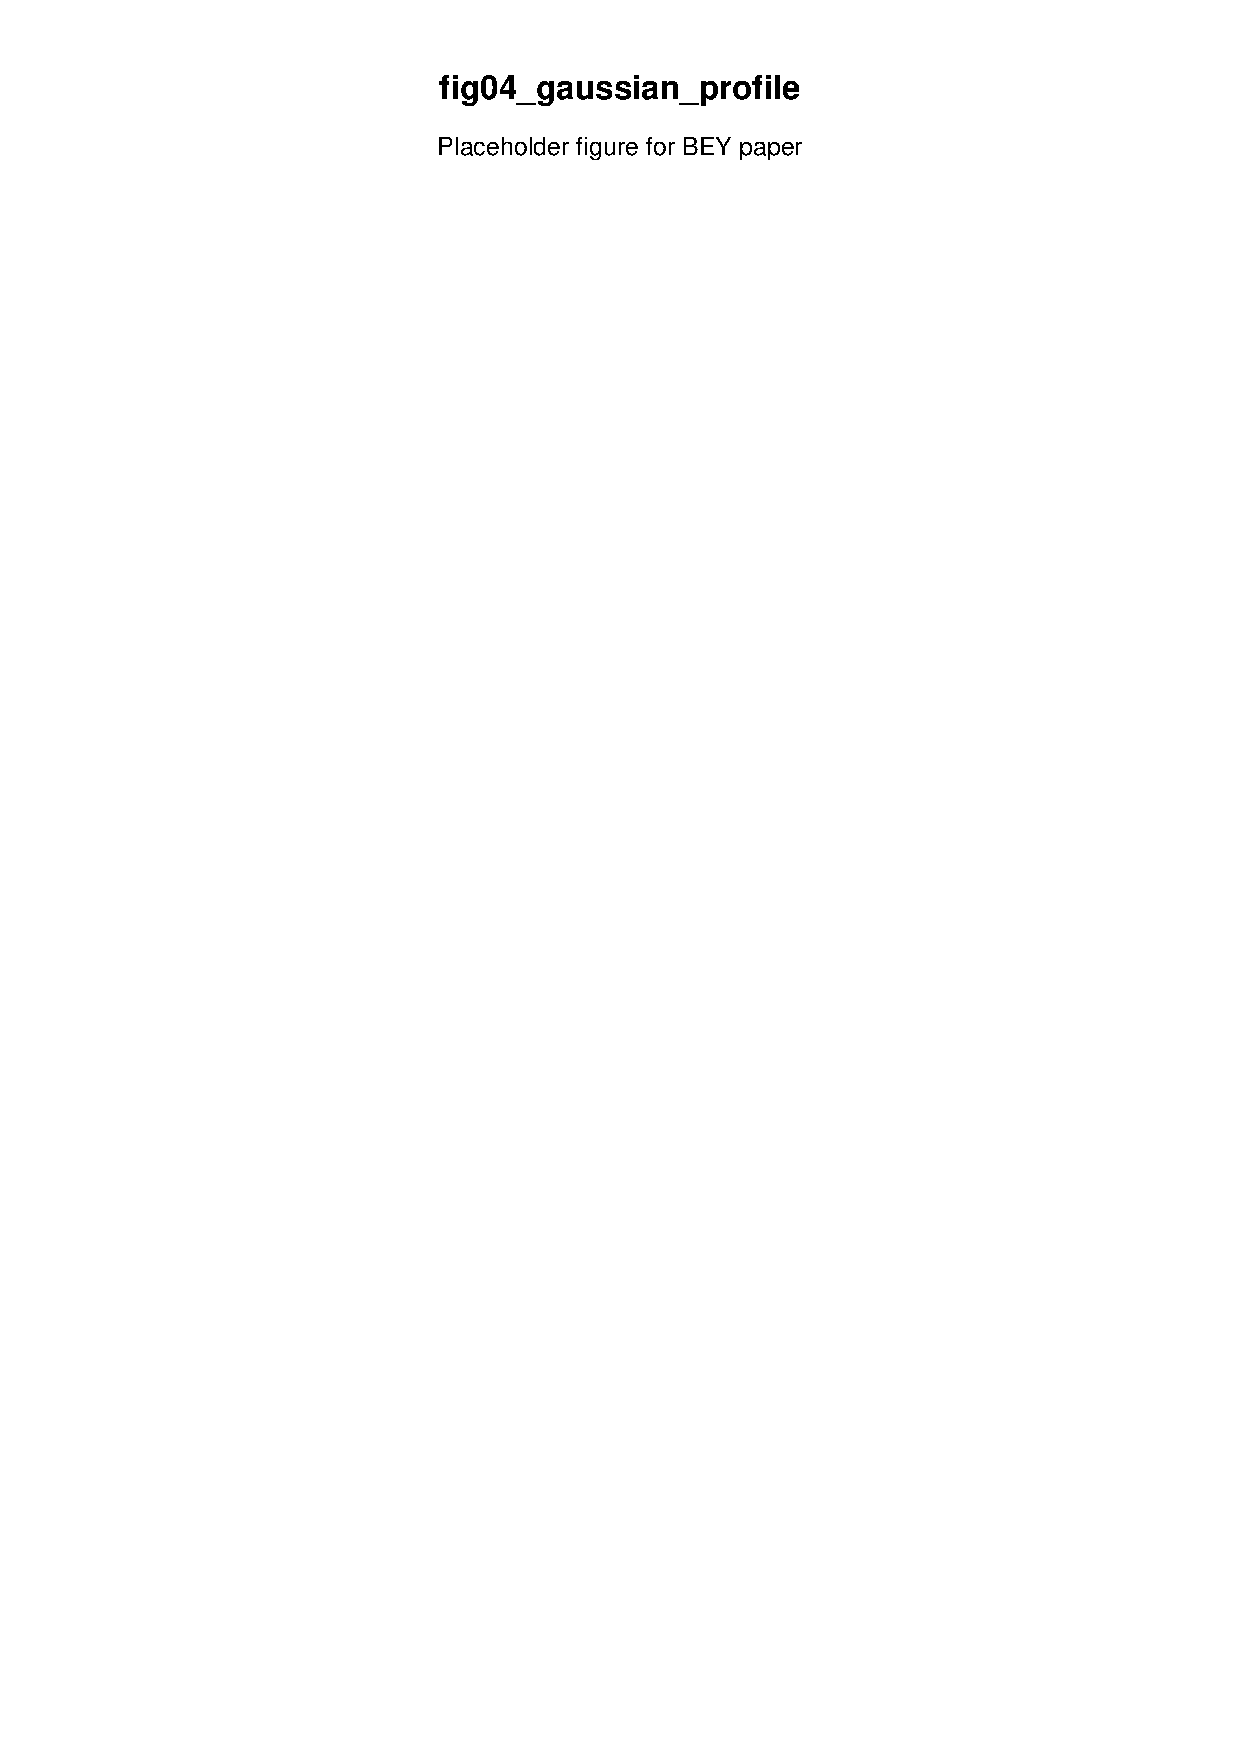
\includegraphics{fig04_gaussian_profile.pdf}
}
\caption{Gaussian condensate profile in the de Sitter harmonic trap. \textbf{Top-left:} density profile of the SC ground state (blue) compared with the divergent classical singularity (red). \textbf{Top-right:} the harmonic-oscillator potential and the Gaussian ground state. \textbf{Bottom-left:} the condensate profile is universal in units of $\sigma$. \textbf{Bottom-right:} characteristic core size $\sigma$ versus mass, compared with $R_s$ and $\ell_{\rm Pl}$.}
\label{fig:gaussian_profile}
\end{figure*}

\subsection{Self-consistent solution: backreaction beyond the de Sitter ansatz}
\label{sec:self_consistent}

To assess the validity of the approximately de Sitter approximation, we solve the coupled effective system as a boundary-value problem (BVP) without imposing constant density. In dimensionless units rescaled by $\sigma_{\rm dS} = \sqrt{\hbar/(m_{\rm pair}\omega_{\rm dS})}$, the stationary equation takes the form
\begin{equation}
-\phi''(\xi) - \frac{2}{\xi}\phi'(\xi) + \xi^2\,\phi(\xi) + \tilde{g}\,\phi^3(\xi) = \tilde{\epsilon}\,\phi(\xi),
\label{eq:GP_dimensionless}
\end{equation}
where $\tilde{g}$ is the dimensionless self-interaction and $\tilde{\epsilon}$ is the eigenvalue. For our fiducial $\tilde{g} = 0.1$, we obtain $\tilde{\epsilon}_0 = 3.0357$, to be compared with the linear three-dimensional harmonic oscillator value $\tilde{\epsilon}_0^{\rm linear} = 3.0$. The nonlinear shift $\Delta\tilde{\epsilon}_0 \approx 1.2\%$ is consistent with the mean-field BEC perturbative estimate. Scanning $\tilde{g}\in[0,0.5]$ supports the expected linear scaling $\Delta\tilde{\epsilon}_0 \approx 0.36\,\tilde{g}$ (Table~\ref{tab:gp_scan}).

\begin{table*}
\centering
\caption{Ground-state eigenvalue $\tilde{\epsilon}_0$ as a function of $\tilde{g}$.}
\label{tab:gp_scan}
\begin{tabular}{cccc}
\hline\noalign{\smallskip}
$\tilde{g}$ & $\tilde{\epsilon}_0$ & $\Delta\tilde{\epsilon}_0$ & Shift [\%] \\
\noalign{\smallskip}\hline\noalign{\smallskip}
0.00 & 3.0000 & $+0.0000$ & $0.0$ \\
0.05 & 3.0178 & $+0.0178$ & $0.6$ \\
0.10 & 3.0357 & $+0.0357$ & $1.2$ \\
0.20 & 3.0719 & $+0.0719$ & $2.4$ \\
0.50 & 3.1845 & $+0.1845$ & $6.1$ \\
\noalign{\smallskip}\hline
\end{tabular}
\end{table*}

The self-consistent profile (Fig.~\ref{fig:einstein_gp}) overlaps with the analytic Gaussian to within graphical precision. Three conclusions follow: (i) the constant-density ansatz is accurate at the percent level; (ii) the condensate is highly localised; (iii) the linear scaling $\tilde{\epsilon}_0(\tilde{g})$ provides a quantitative parameter sensitivity check.

\begin{figure*}
\resizebox{0.92\textwidth}{!}{%
  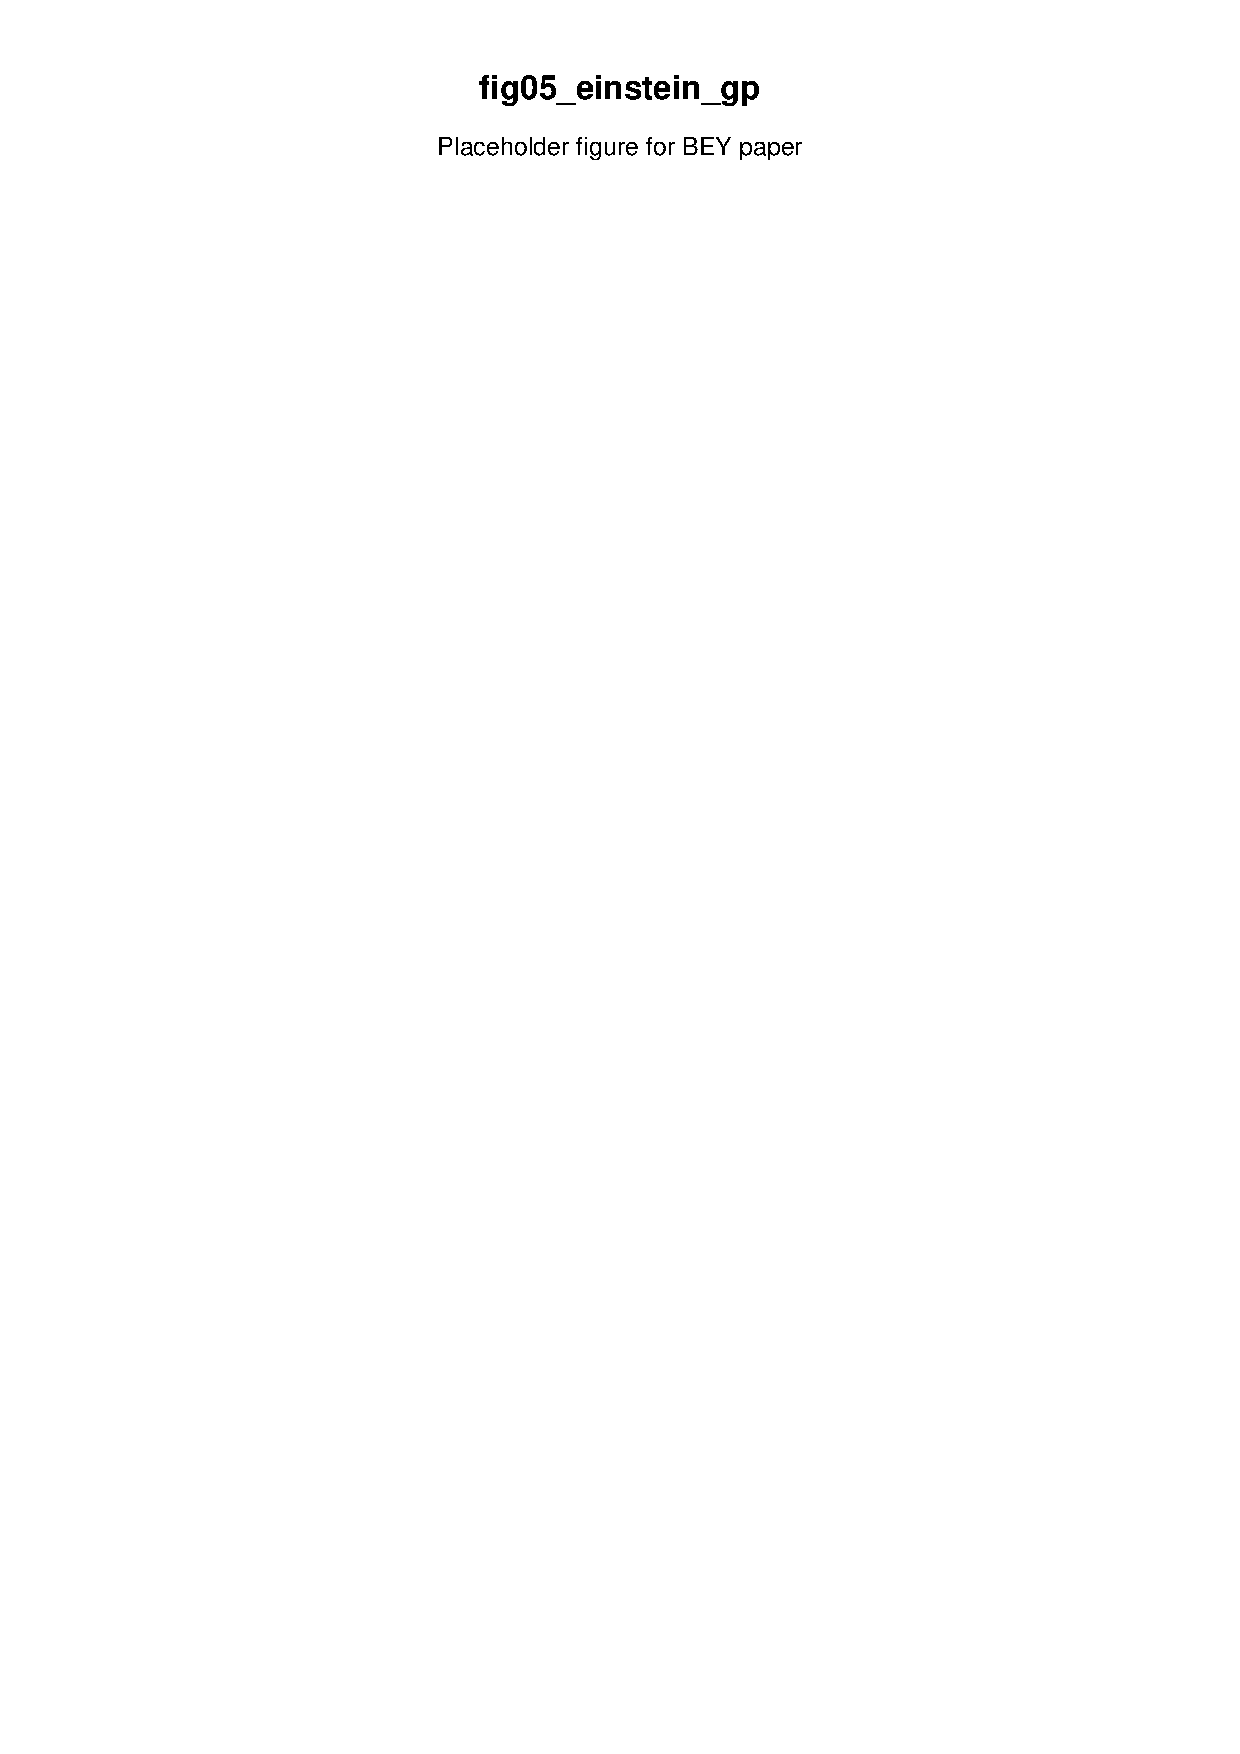
\includegraphics{fig05_einstein_gp.pdf}
}
\caption{Self-consistent solution of the coupled effective system in the de Sitter harmonic trap. \textbf{Top-left:} ground-state amplitude (BVP) vs.\ linear analytic ground state. \textbf{Top-right:} energy density profile (log scale). \textbf{Bottom-left:} enclosed mass. \textbf{Bottom-right:} profiles for a range of $\tilde{g}$.}
\label{fig:einstein_gp}
\end{figure*}

\subsection{Linear stability analysis}
\label{sec:stability}

We test linear dynamical stability, within the Cowling approximation, by computing the Bogoliubov--de Gennes (BdG) spectrum of fluctuations around the self-consistent ground state $\phi_0(\xi)$. Writing $\phi(\xi,t) = \phi_0(\xi) + \delta\phi(\xi,t)$ and linearising Eq.~\eqref{eq:GP_dimensionless} yields the standard BdG eigenvalue problem
\begin{equation}
\hat{H}^2\, u_n(\xi) = \omega_n^2\, u_n(\xi),
\qquad
\hat{H}^2 \equiv (\hat{L} + \hat{M})(\hat{L} - \hat{M}),
\label{eq:BdG}
\end{equation}
with $\hat{L} = -\nabla^2 + \xi^2 - \tilde\mu + 2\tilde{g}\,\phi_0^2$ and $\hat{M} = \tilde{g}\,\phi_0^2$. We adopt a Cowling-type analysis in which the background metric is held fixed; coupled metric-condensate perturbations are deferred to future work.

To avoid spurious boundary modes, we expand in numerically constructed orthonormal 3D $s$-wave Hermite--Gauss functions ($N=30$, verified by convergence tests against $N=20, 40$, with eigenvalues stable to better than $10^{-4}$). The results (Fig.~\ref{fig:stability}) show: one Goldstone mode at numerical precision ($|\omega_0^2| < 10^{-3}$, consistent with the U(1) broken symmetry); 29 stable physical modes ($\omega_n^2 > 0$); no genuine instabilities. The dimensionless sound speed $c_s^2 = \tilde{g}|\phi_0(0)|^2 = 0.10$ ($c_s/c \simeq 0.32$) is positive.

\begin{figure*}
\resizebox{0.92\textwidth}{!}{%
  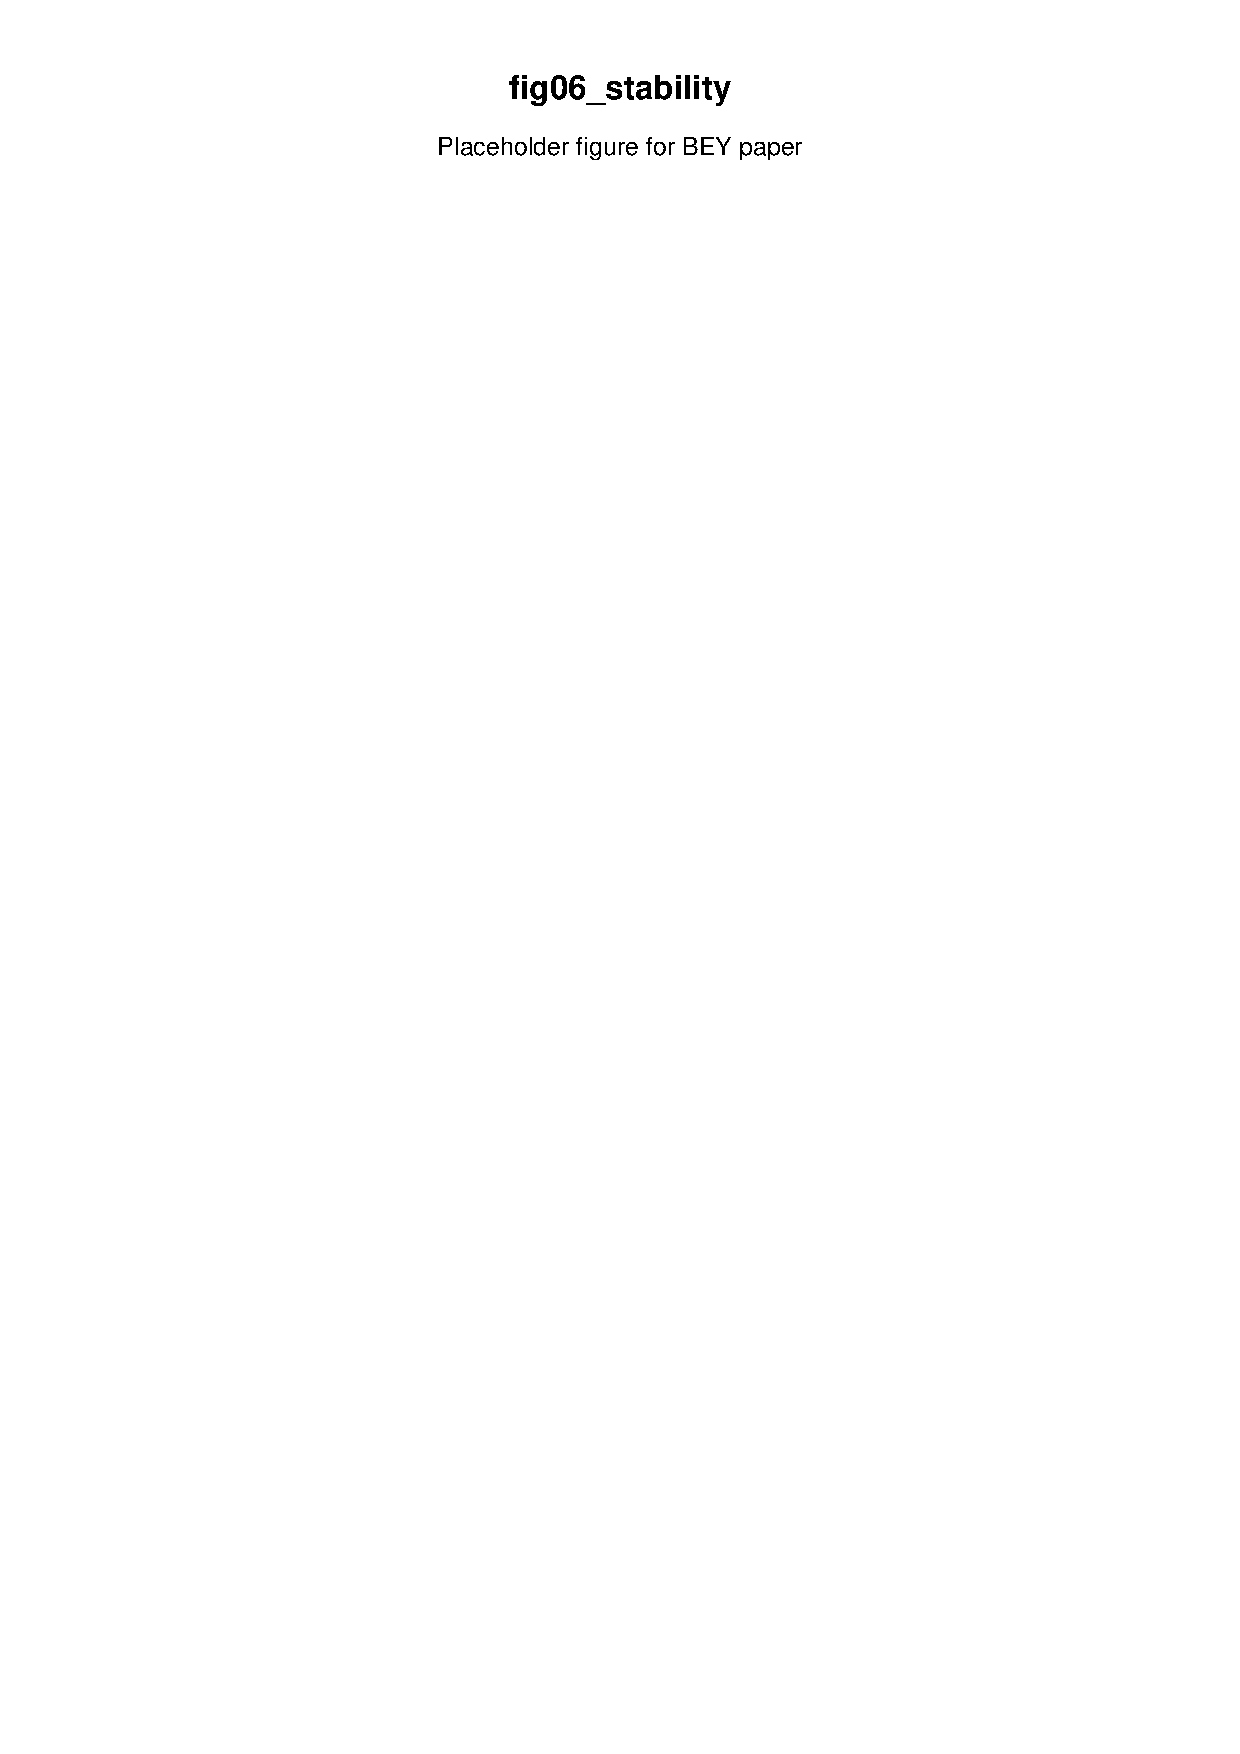
\includegraphics{fig06_stability.pdf}
}
\caption{Linear stability analysis via Bogoliubov--de Gennes spectrum (Cowling approximation). \textbf{Top-left:} spectrum, with one Goldstone mode (grey) and 29 stable modes (blue). \textbf{Top-right:} lowest mode profiles. \textbf{Bottom-left:} numerical eigenfrequencies vs.\ analytic HO. \textbf{Bottom-right:} ground state with lowest stable mode.}
\label{fig:stability}
\end{figure*}

\subsection{Phase--Spectral Stability of the Schwarzschild Condensate}
\label{subsec:phase_spectral_sc}

The preceding subsections established three ingredients of the Schwarzschild
Condensation (SC) scenario: a QCD-motivated transition to a color-superconducting phase, a regular approximately de Sitter interior, and a linearly stable Bogoliubov--de Gennes spectrum. In this subsection we collect these results into a single phase--spectral stability criterion. The purpose is not to introduce a new microscopic assumption, but to make explicit the mathematical structure that connects the condensate order parameter, the regularity of the geometry, the positive perturbation spectrum, and the possible ECO echo/ringdown phenomenology.

\paragraph{Notation.}
Throughout this subsection, the subscript ``SC'' refers only to the
Schwarzschild Condensation compact-object model. The quantities
$\Phi_{\rm SC}$, $\Delta_{\rm SC}$, and $\mathcal{O}_{\rm SC}$ therefore denote, respectively, the condensate order parameter, the condensate fluctuation gap, and the compact-object perturbation operator. They should not be confused with gauge-theory or cosmological quantities carrying analogous phase--spectral roles.

We define the SC phase data by
\begin{equation}
\mathfrak{P}_{\rm SC}
=
\left(
\mathcal{D}_{\rm SC},
\lambda_{\rm SC},
\Phi_{\rm SC},
V_{\rm SC},
\mathcal{O}_{\rm SC},
\Delta_{\rm SC},
\mathcal{M}_{\rm SC}
\right),
\label{eq:SC_phase_data}
\end{equation}
where $\mathcal{D}_{\rm SC}$ is the interior domain, $\lambda_{\rm SC}$ denotes
the collapse-control parameters, $\Phi_{\rm SC}$ is the condensate order
parameter, $V_{\rm SC}$ is the effective core potential, $\mathcal{O}_{\rm SC}$
is the fluctuation operator, $\Delta_{\rm SC}$ is the corresponding spectral
stability gap, and $\mathcal{M}_{\rm SC}$ maps the interior phase data to
observable quantities.

The relevant control parameters are taken to be
\begin{equation}
\lambda_{\rm SC}
=
\left(
\rho(r),
\mu_q(r),
n_B(r),
K(r),
r
\right),
\label{eq:SC_control_parameters}
\end{equation}
where $\rho(r)$ is the local energy density, $\mu_q(r)$ is the quark chemical
potential, $n_B(r)$ is the baryon number density, and
\begin{equation}
K(r)
=
R_{\mu\nu\rho\sigma}R^{\mu\nu\rho\sigma}
\label{eq:SC_kretschmann}
\end{equation}
is the Kretschmann scalar. The SC phase is activated when the local dense-matter
conditions enter the QCD regime,
\begin{equation}
\mu_q(r) \gtrsim \Lambda_{\rm QCD},
\qquad
n_B(r) \gtrsim n_{\rm trans},
\qquad
\xi_{\rm CFL} \ll L_{\rm core},
\label{eq:SC_activation_conditions}
\end{equation}
where $n_{\rm trans}$ is the hadron--quark transition density obtained from the
MIT bag plus CFL pairing analysis, $\xi_{\rm CFL}$ is the CFL coherence length,
and $L_{\rm core}$ is the characteristic density-gradient scale of the interior.
These inequalities express the transition from ordinary hadronic matter to a
macroscopic Cooper-paired quark condensate.

The condensate phase is represented by a complex scalar order parameter,
\begin{equation}
\Phi_{\rm SC}(r)
\equiv
|\Psi(r)| e^{i\theta(r)},
\label{eq:SC_order_parameter}
\end{equation}
with $\Phi_{\rm SC}=0$ in the uncondensed phase and
$\Phi_{\rm SC}\neq 0$ in the color-superconducting phase. Equivalently, the
microscopic CFL pairing condition may be written schematically as
\begin{equation}
\langle q^a_{\alpha} q^b_{\beta} \rangle \neq 0,
\label{eq:SC_pairing_order}
\end{equation}
where color and flavor indices are suppressed. In the long-wavelength effective
description this pairing condensate is encoded by $\Psi$.

A minimal effective potential for the SC order parameter may be written as
\begin{equation}
\begin{aligned}
V_{\rm SC}(|\Psi|;r)
&=
\alpha_{\rm SC}(r)|\Psi|^2
+
\frac{\lambda_{\rm SC}}{2}|\Psi|^4
+
V_{\rm core}(r),\\
&\hspace{2em}\lambda_{\rm SC}>0 .
\end{aligned}
\label{eq:SC_effective_potential}
\end{equation}
The phase transition corresponds to a sign change of the quadratic coefficient,
\begin{equation}
\alpha_{\rm SC}(r)
\begin{cases}
>0, & \text{outside the condensed phase},\\
<0, & \text{inside the condensed core}.
\end{cases}
\label{eq:SC_alpha_sign}
\end{equation}
For $\alpha_{\rm SC}<0$, the non-trivial minimum is
\begin{equation}
|\Psi_0(r)|^2
=
-\frac{\alpha_{\rm SC}(r)}{\lambda_{\rm SC}},
\label{eq:SC_condensate_minimum}
\end{equation}
and local phase stability requires
\begin{equation}
\left.
\frac{\partial^2 V_{\rm SC}}{\partial |\Psi|^2}
\right|_{\Psi=\Psi_0}
> 0 .
\label{eq:SC_potential_stability}
\end{equation}
This condition is the effective-potential expression of the fact that the
condensed configuration is a true local minimum rather than a transient
tachyonic instability.

The geometric regularity condition is independent of the microscopic pairing
description. A nonsingular SC interior must satisfy
\begin{equation}
\lim_{r\rightarrow 0}\rho_{\rm eff}(r)=\rho_0<\infty,
\qquad
\lim_{r\rightarrow 0}p_{\rm eff}(r)=p_0<\infty,
\label{eq:SC_finite_stress_energy}
\end{equation}
and
\begin{equation}
\lim_{r\rightarrow 0}K(r)=K_0<\infty .
\label{eq:SC_finite_kretschmann}
\end{equation}
For the approximately de Sitter core used in this work, the density is bounded
and the central curvature invariant remains finite. Thus the classical
Schwarzschild divergence is replaced by a finite-density endpoint.

The spectral part of the criterion is obtained by perturbing the condensate
around the self-consistent ground state,
\begin{equation}
\Psi(r,t)
=
\Psi_0(r)
+
\delta\Psi(r,t),
\label{eq:SC_perturbation}
\end{equation}
and expanding the fluctuation in Bogoliubov modes,
\begin{equation}
\delta\Psi(r,t)
=
u_n(r)e^{-i\omega_n t}
+
v_n^*(r)e^{i\omega_n t}.
\label{eq:SC_bdg_expansion}
\end{equation}
The corresponding BdG eigenvalue problem may be written schematically as
\begin{equation}
\mathcal{O}_{\rm BdG}
\begin{pmatrix}
u_n\\
v_n
\end{pmatrix}
=
\hbar\omega_n
\begin{pmatrix}
u_n\\
v_n
\end{pmatrix},
\label{eq:SC_bdg_operator}
\end{equation}
where $\mathcal{O}_{\rm BdG}$ is the linearised fluctuation operator around the
SC ground state. The Goldstone mode associated with the broken phase symmetry is
excluded from the stability floor. We therefore define the SC spectral gap by
\begin{equation}
\Delta_{\rm SC}
=
\inf_{n\notin\mathcal{G}}
\omega_n^2 ,
\label{eq:SC_spectral_gap}
\end{equation}
where $\mathcal{G}$ denotes the Goldstone sector. Linear dynamical stability
requires
\begin{equation}
\Delta_{\rm SC}>0 .
\label{eq:SC_positive_gap}
\end{equation}
Equivalently, the BdG spectrum must contain no negative $\omega_n^2$ modes.
This is precisely the condition tested numerically in the preceding stability
analysis.

Combining the phase, geometric, and spectral requirements, the SC model is
phase--spectrally stable if the following four conditions are satisfied:
\begin{center}
\refstepcounter{equation}
\label{eq:SC_phase_spectral_criterion}
\fbox{%
\begin{minipage}{0.82\columnwidth}
\centering
\vspace{2pt}
$\Phi_{\rm SC}\neq 0,\qquad
\xi_{\rm CFL}\ll L_{\rm core}$

\vspace{4pt}

$K_0<\infty,\qquad
\Delta_{\rm SC}>0$
\vspace{2pt}
\end{minipage}%
}
\hfill(\theequation)
\end{center}
with the additional requirement that the resulting phase data possess an
observable map. In the ECO interpretation this map is
\begin{equation}
\mathcal{M}_{\rm SC}:
\left(
\Phi_{\rm SC},
\Delta_{\rm SC},
R_0,
\delta
\right)
\longmapsto
\left(
\omega_{\rm QNM},
\Delta t_{\rm echo},
\mathcal{A}_{\rm echo},
\delta f_R
\right),
\label{eq:SC_observable_map}
\end{equation}
where $R_0=R_s(1+\delta)$ is the effective reflecting surface, $\omega_{\rm QNM}$
is the ringdown frequency, $\Delta t_{\rm echo}$ is the echo delay,
$\mathcal{A}_{\rm echo}$ is the echo amplitude, and $\delta f_R$ denotes the
frequency shift relative to the classical black-hole prediction.

For a near-horizon reflecting surface the echo delay is controlled, to leading
order, by the optical length of the exterior cavity,
\begin{equation}
\Delta t_{\rm echo}
\simeq
\frac{2}{c}
\int_{R_0}^{r_{\rm peak}}
dr_*,
\qquad
r_*
=
r
+
R_s\ln\left|
\frac{r}{R_s}-1
\right| ,
\label{eq:SC_echo_delay_map}
\end{equation}
where $r_{\rm peak}$ is the approximate location of the angular-momentum barrier.
The interior condensate affects this map through the boundary condition at
$R_0$, the stiffness of the core, and the positive BdG spectrum.

It is important to stress that $\Delta_{\rm SC}$ is not a Yang--Mills mass gap
and is not being identified with any cosmological spectral gap. It is the
positive fluctuation gap of the SC condensate in the effective compact-object
interior. The common role of the gap is structural: in each case a positive
spectral floor suppresses unstable long-wavelength modes and supports a stable
phase. Thus the SC construction provides a concrete compact-object realization
of the broader phase--spectral idea, while remaining a phenomenological,
QCD-inspired model rather than a derived theory of quantum gravity.

\paragraph{Assumptions and validity domain.}
The phase--spectral SC criterion is valid only within the effective
compact-object regime considered in this work. It assumes that the local
collapse dynamics reaches the QCD deconfinement domain, that CFL-like pairing can be represented by a long-wavelength condensate order parameter, that the condensate stress--energy supports a bounded central geometry, and that the linearised Bogoliubov--de Gennes analysis captures the leading stability properties of the core. If any of these assumptions fails, the criterion should not be interpreted as evidence for a regular SC interior. In particular, the condition $\Delta_{\rm SC}>0$ establishes only linear spectral stability of the effective condensate background; it does not by itself prove nonlinear stability or provide a microscopic derivation from full quantum gravity.

\paragraph{Connection to later sections.}
The phase--spectral criterion summarized here provides the internal bridge to the observational analysis in Sect.~12. The quantities entering $\mathcal{M}_{\rm SC}$ should therefore be read as the compact-object translation of the same core data: the condensate order parameter fixes the interior phase, the positive BdG spectrum fixes linear stability, and the near-surface boundary condition controls the possible echo and ringdown response in the ECO interpretation.


\subsection{Energy-condition, tapered-boundary, and curvature diagnostics}
\label{sec:regular_core_diagnostics}

The preceding construction motivates a regular finite-density core, but the
phenomenological ansatz must also pass basic consistency filters. We therefore
supplement the analytic de Sitter-core and BdG calculations with three numerical
diagnostic scans. These scans should be read as effective-core consistency tests,
not as a full Einstein--QCD solution and not as a complete non-linear stability
proof.

We use a dimensionless radial coordinate $x=r/R_c$ and begin from the bounded
regular-core profile
\begin{equation}
\rho(x)=\frac{\rho_c}{1+x^4},
\label{eq:diagnostic_rho_untapered}
\end{equation}
with enclosed mass
\begin{equation}
m(x)=4\pi\rho_c R_c^3 I(x),\qquad
I(x)=\int_0^x \frac{u^2}{1+u^4}\,du .
\label{eq:diagnostic_mass_function}
\end{equation}
The corresponding single-function metric diagnostic is written as
\begin{equation}
f(x)=1-A\frac{I(x)}{x},
\qquad
A=8\pi\rho_c R_c^2,
\label{eq:diagnostic_metric_function}
\end{equation}
where $A$ controls the effective compactness of the core. Near the origin
$I(x)\sim x^3/3$, so $m(r)\sim r^3$ and the central metric is regular at the
level of this ansatz.

For the stress--energy diagnostic we use an anisotropic effective-fluid form
$T^\mu{}_{\nu}=\mathrm{diag}(-\rho,p_r,p_t,p_t)$ with
\begin{equation}
p_r=w\rho,
\qquad
p_t=p_r+\alpha\rho\frac{x^2}{1+x^2}.
\label{eq:diagnostic_pressures}
\end{equation}
The null, weak, strong, and dominant energy-condition filters are evaluated as
\begin{align}
\rho+p_r&\geq 0,\qquad \rho+p_t\geq 0,
\label{eq:diagnostic_nec}\\
\rho&\geq0,
\label{eq:diagnostic_wec}\\
\rho+p_r+2p_t&\geq0,
\label{eq:diagnostic_sec}\\
\rho-|p_r|&\geq0,\qquad \rho-|p_t|\geq0 .
\label{eq:diagnostic_dec}
\end{align}
The untapered scan contains 60 parameter sets. All 60 have a regular centre; 56
satisfy NEC, WEC, and DEC; 32 satisfy SEC; 8 pass the strict causal-proxy filter;
and 56 pass the broader regularizing-core filter. The only failures occur in
aggressively negative-pressure anisotropic branches, which are not used as the
fiducial SC branch.

The untapered profile is useful as a baseline, but it generically leaves a
non-zero effective boundary pressure at a finite matching radius. To reduce this
matching tension we introduce a tapered branch
\begin{equation}
\begin{aligned}
\rho_{\rm tap}(x)
&=
\frac{\rho_c}{1+x^4}\,S_q(x),
\\
S_q(x)
&=
\begin{cases}
\left[1-(x/x_m)^2\right]^q, & x<x_m,\\
0, & x\geq x_m .
\end{cases}
\end{aligned}
\label{eq:diagnostic_tapered_profile}
\end{equation}
where $x_m=R_{\rm match}/R_c$ is the matching surface and $q$ controls the
taper sharpness. This branch enforces
\begin{equation}
\rho_{\rm tap}(x_m)=p_r(x_m)=p_t(x_m)=0,
\label{eq:diagnostic_boundary_soft}
\end{equation}
so that the exterior can be interpreted as Schwarzschild vacuum without an
artificial residual pressure at the interface. In the 288-set tapered scan, all
sets pass NEC, WEC, SEC, DEC, centre-regularity, and boundary-softness filters;
240 pass the strict causal-proxy filter. The mean absolute boundary pressure is
reduced from $1.77\times10^{-3}$ in the untapered comparison to
$1.92\times10^{-10}$ in the tapered branch, and the thin-shell warning count is
reduced from $12/12$ to $0/12$ in the matching comparison.

\begin{table*}
\centering
\caption{Effective-core diagnostic summary. ``Strict'' includes the causal-proxy filter, while ``regularizing'' keeps the energy-condition and centre/boundary regularity filters without requiring the strict sound-speed proxy for every anisotropic branch.}
\label{tab:effective_core_diagnostics}
\scriptsize
\begin{tabular}{lcccccccc}
\toprule
Scan & Sets & NEC & WEC & SEC & DEC & Centre & Boundary & Strict/Regularizing\\
\midrule
Untapered energy scan & 60 & 56 & 56 & 32 & 56 & 60 & -- & 8 / 56\\
Tapered boundary scan & 288 & 288 & 288 & 288 & 288 & 288 & 288 & 240 / 288\\
Curvature/compactness scan & 96 & -- & -- & -- & -- & 96 & -- & finite curvature: 96\\
\bottomrule
\end{tabular}
\end{table*}

Figure~\ref{fig:tapered_energy_diagnostics} shows the fiducial tapered branch.
The density and pressure vanish smoothly at $x_m$, while the NEC and DEC
diagnostics remain non-negative in the representative branch
$(A,w,\alpha,x_m,q)=(1.0,0.3,0.0,4.0,2)$.

\begin{figure*}
\centering
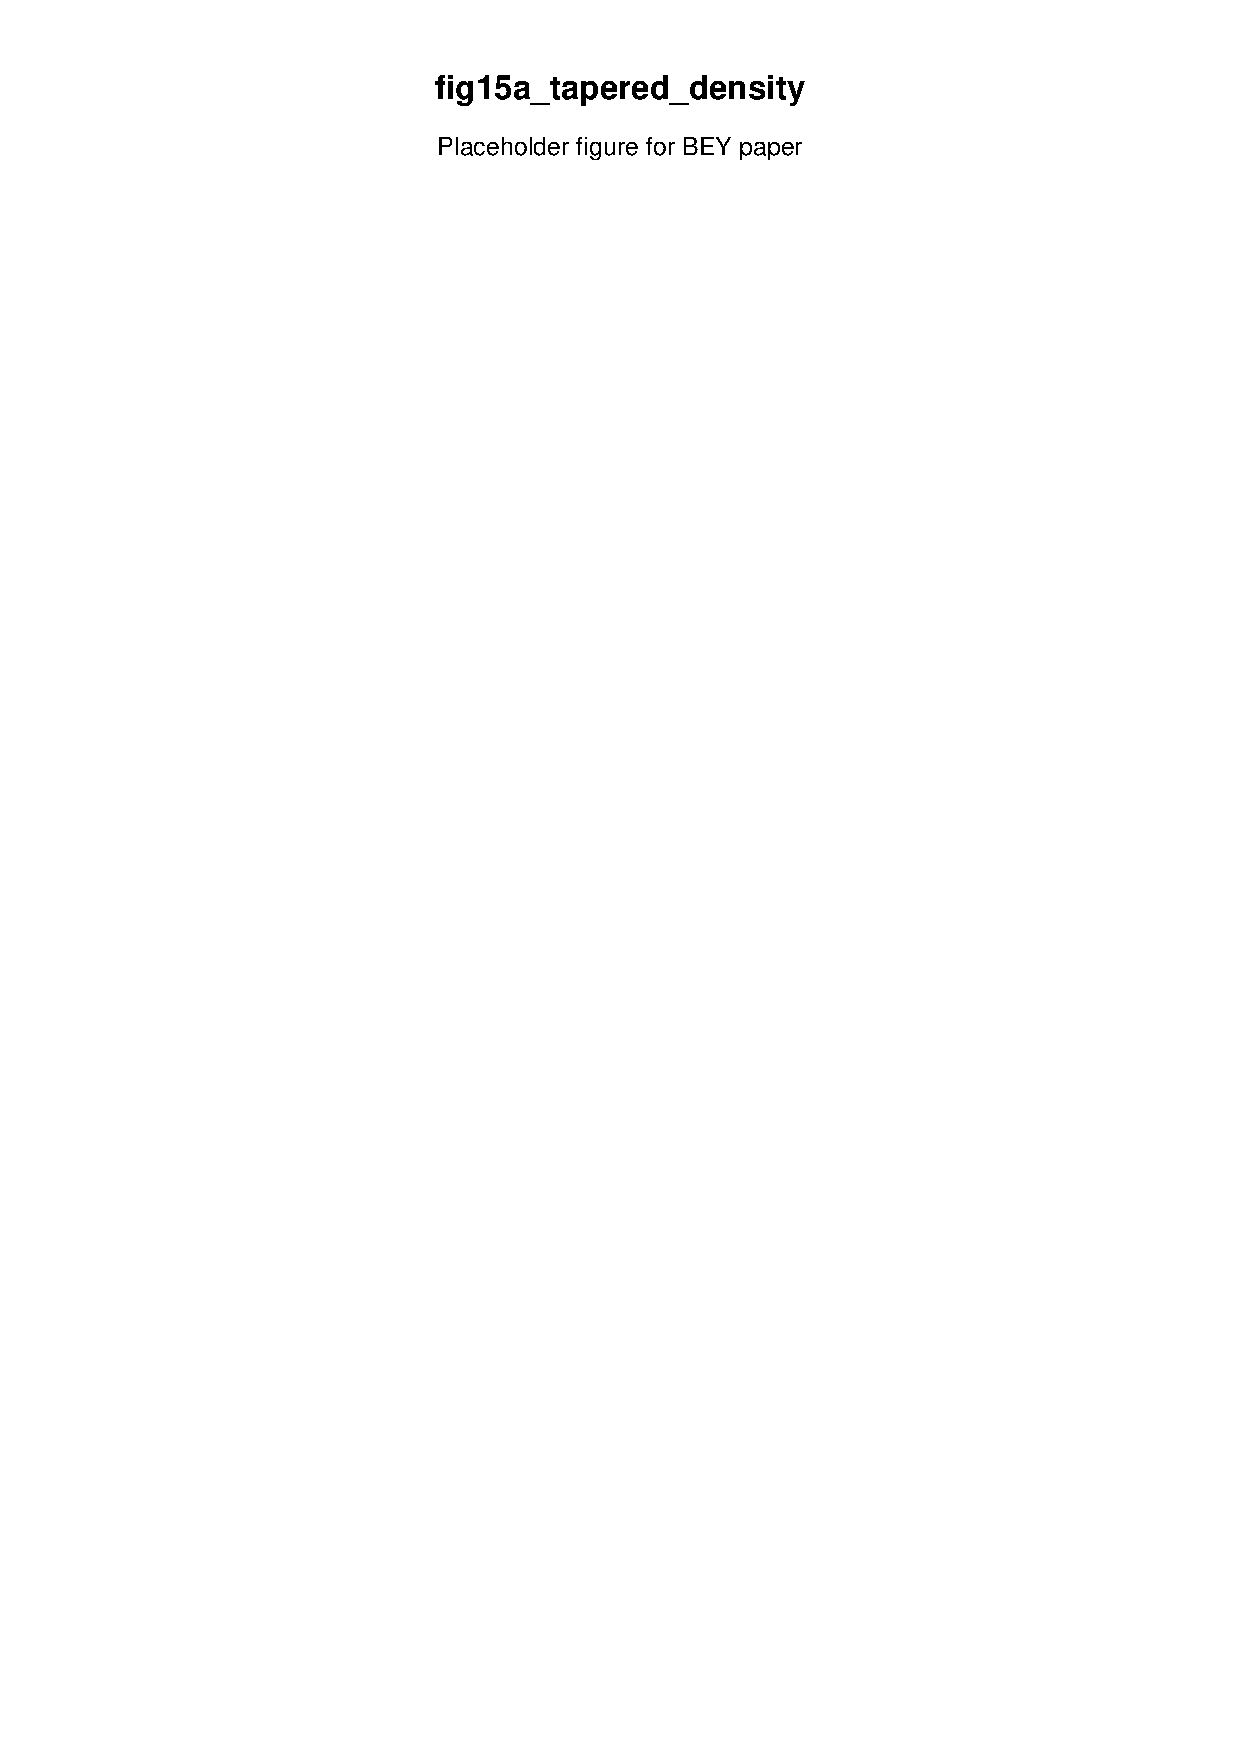
\includegraphics[width=0.48\textwidth]{fig15a_tapered_density.pdf}\hfill
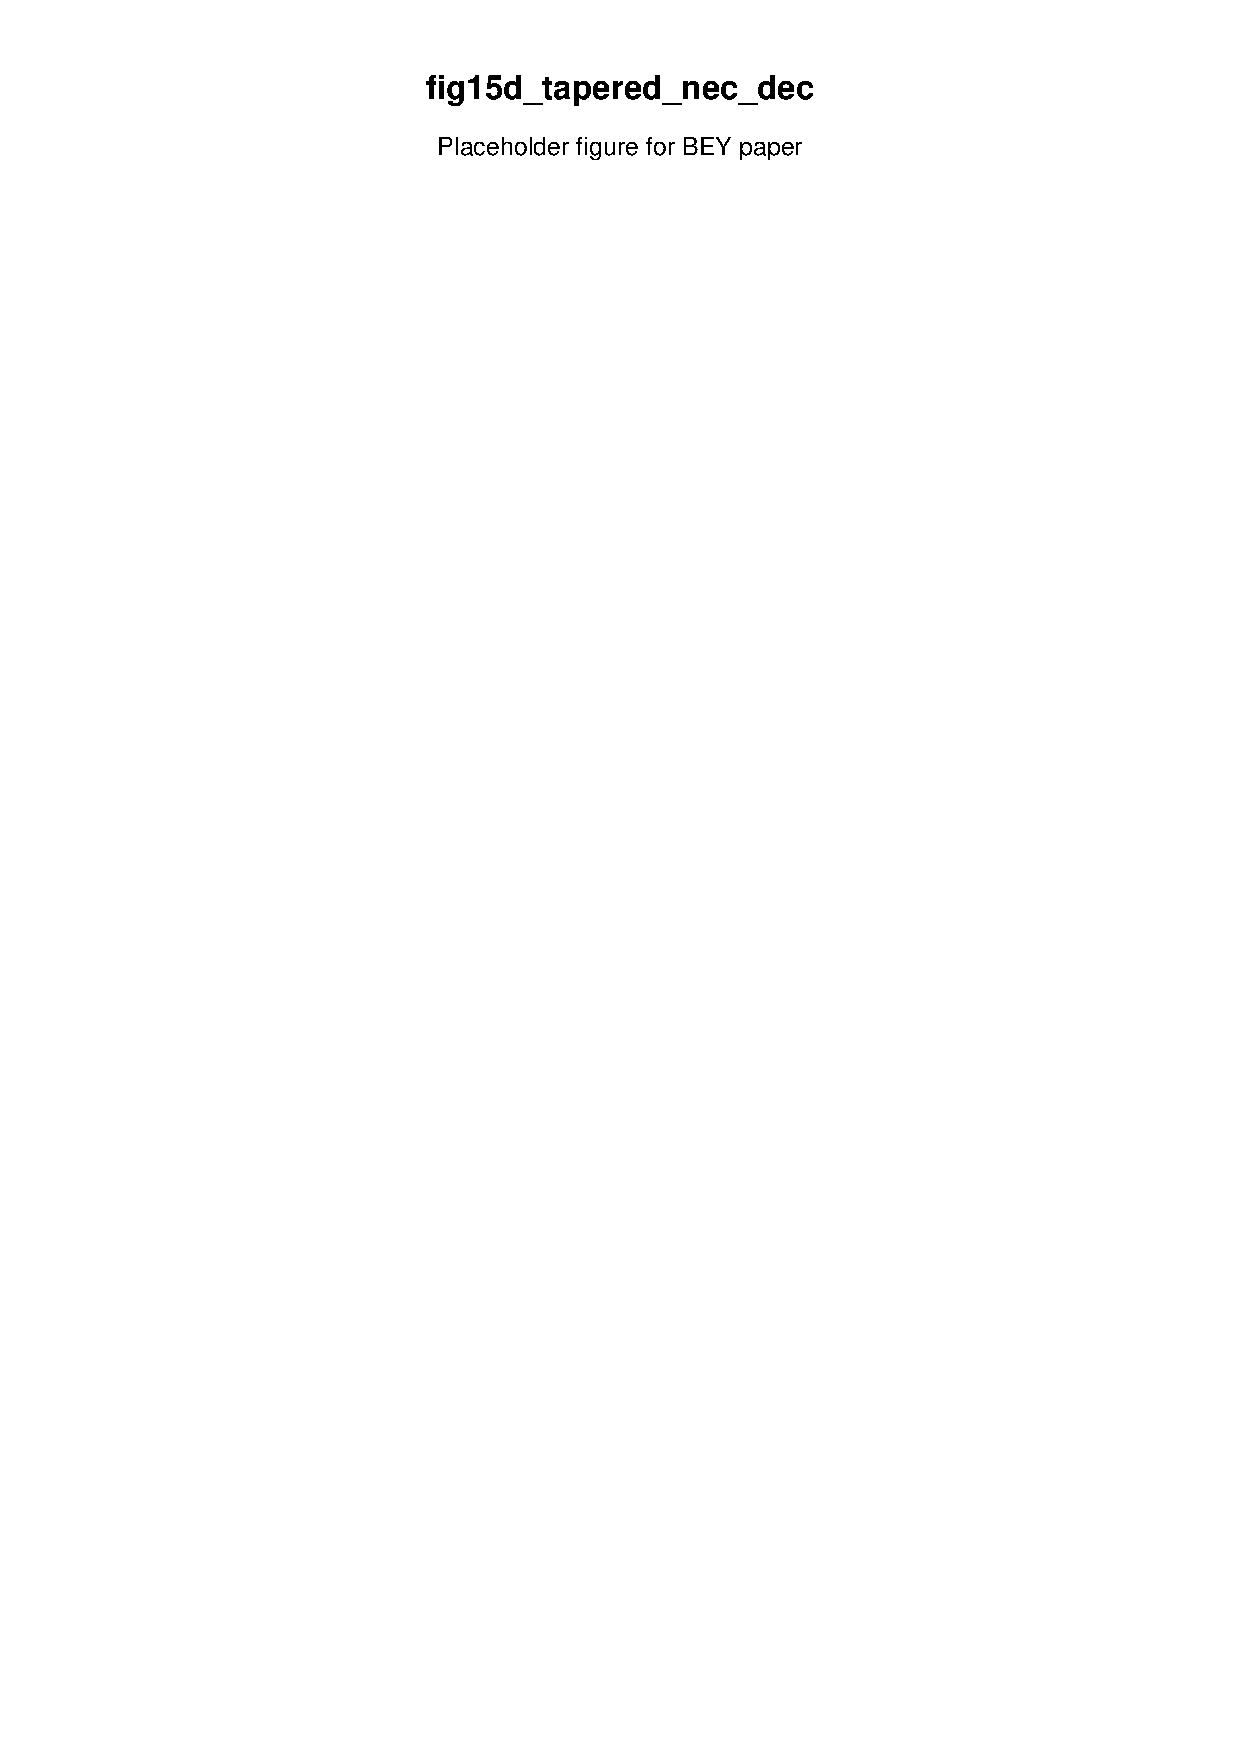
\includegraphics[width=0.48\textwidth]{fig15d_tapered_nec_dec.pdf}
\caption{Tapered regular-core diagnostics. Left: the tapered density profile smoothly approaches zero at the matching surface. Right: representative NEC and DEC diagnostics for the fiducial positive-pressure branch.}
\label{fig:tapered_energy_diagnostics}
\end{figure*}

\begin{figure*}
\centering
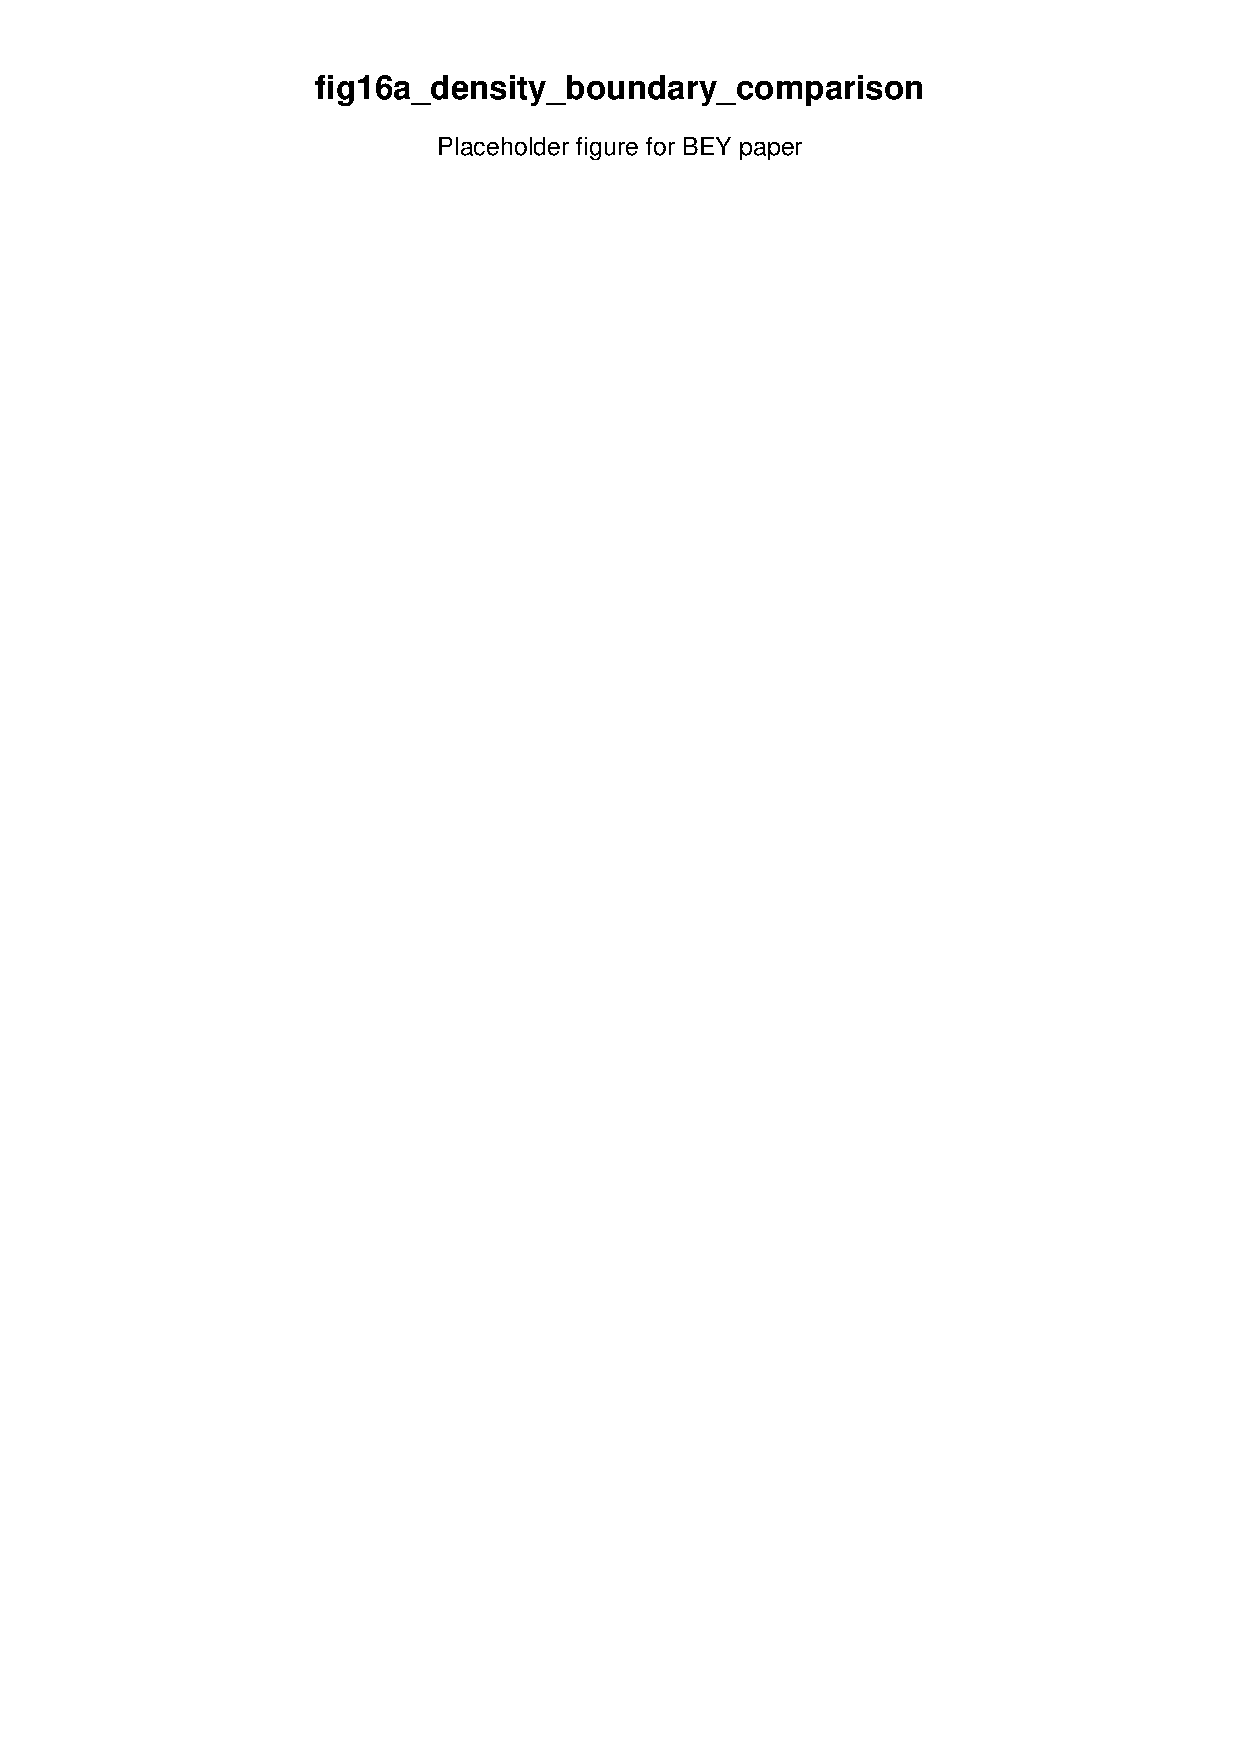
\includegraphics[width=0.48\textwidth]{fig16a_density_boundary_comparison.pdf}\hfill
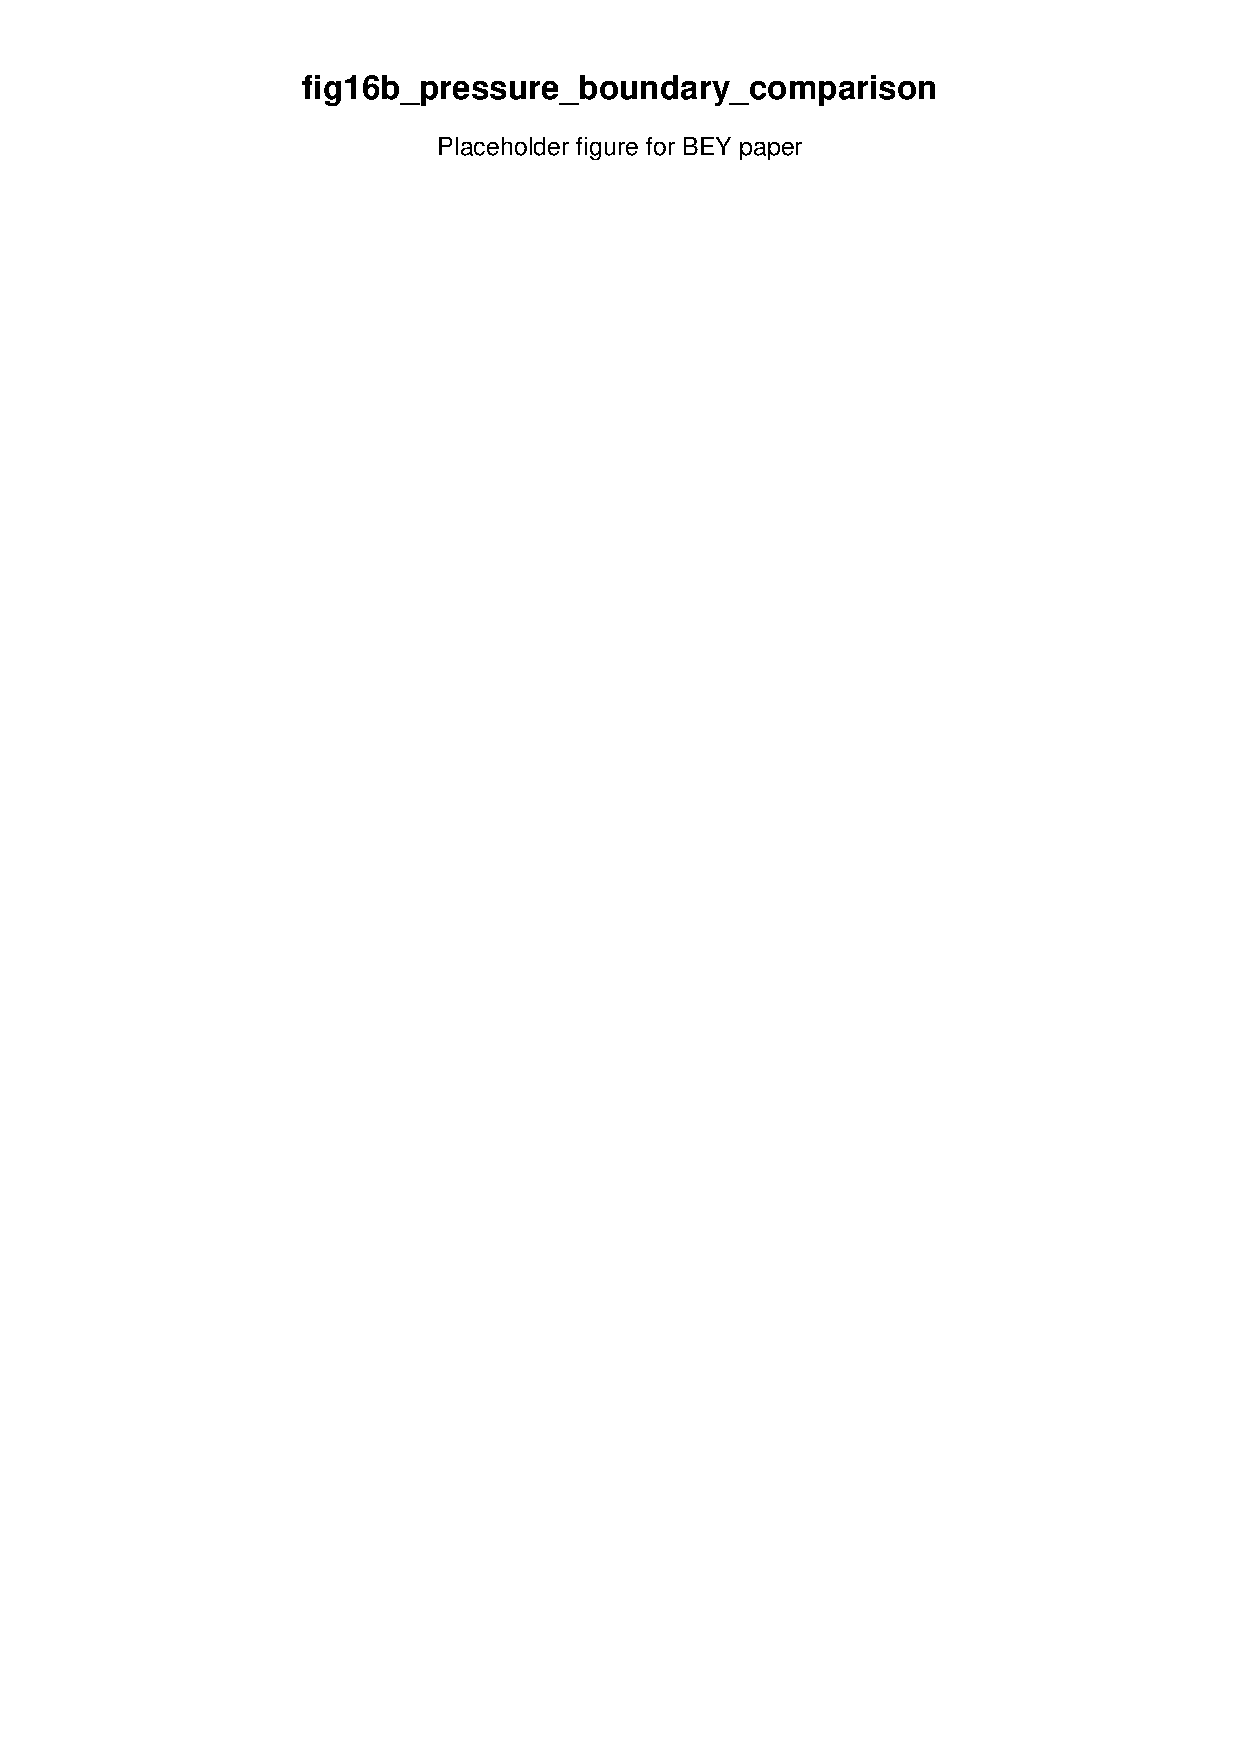
\includegraphics[width=0.48\textwidth]{fig16b_pressure_boundary_comparison.pdf}
\caption{Untapered versus tapered matching diagnostics. The tapered branch suppresses both the effective density and radial pressure at the matching surface, thereby reducing the boundary-pressure tension that appears in the untapered branch.}
\label{fig:tapered_matching_diagnostics}
\end{figure*}

We also evaluate curvature diagnostics for the single-function effective metric.
For
\begin{equation}
ds^2=-f(x)dt^2+\frac{dx^2}{f(x)}+x^2d\Omega^2,
\label{eq:diagnostic_single_function_metric}
\end{equation}
the Ricci-scalar and Kretschmann-like indicators are
\begin{align}
R(x)&=-f''-\frac{4f'}{x}+\frac{2(1-f)}{x^2},
\label{eq:diagnostic_ricci}\\
K_{\rm proxy}(x)&=(f'')^2+4\left(\frac{f'}{x}\right)^2
+4\left(\frac{1-f}{x^2}\right)^2 .
\label{eq:diagnostic_kproxy}
\end{align}
These expressions reproduce the expected finite de Sitter-like behaviour for a
regular centre and vanish appropriately for the Schwarzschild exterior in the
corresponding vacuum limit. In the 96-case curvature/compactness scan, all cases
have finite curvature indicators and pass the regular-centre proxy. This supports
the interpretation of the ansatz as a finite-curvature replacement of the
classical $r=0$ endpoint at the toy-model level.

\begin{figure*}
\centering
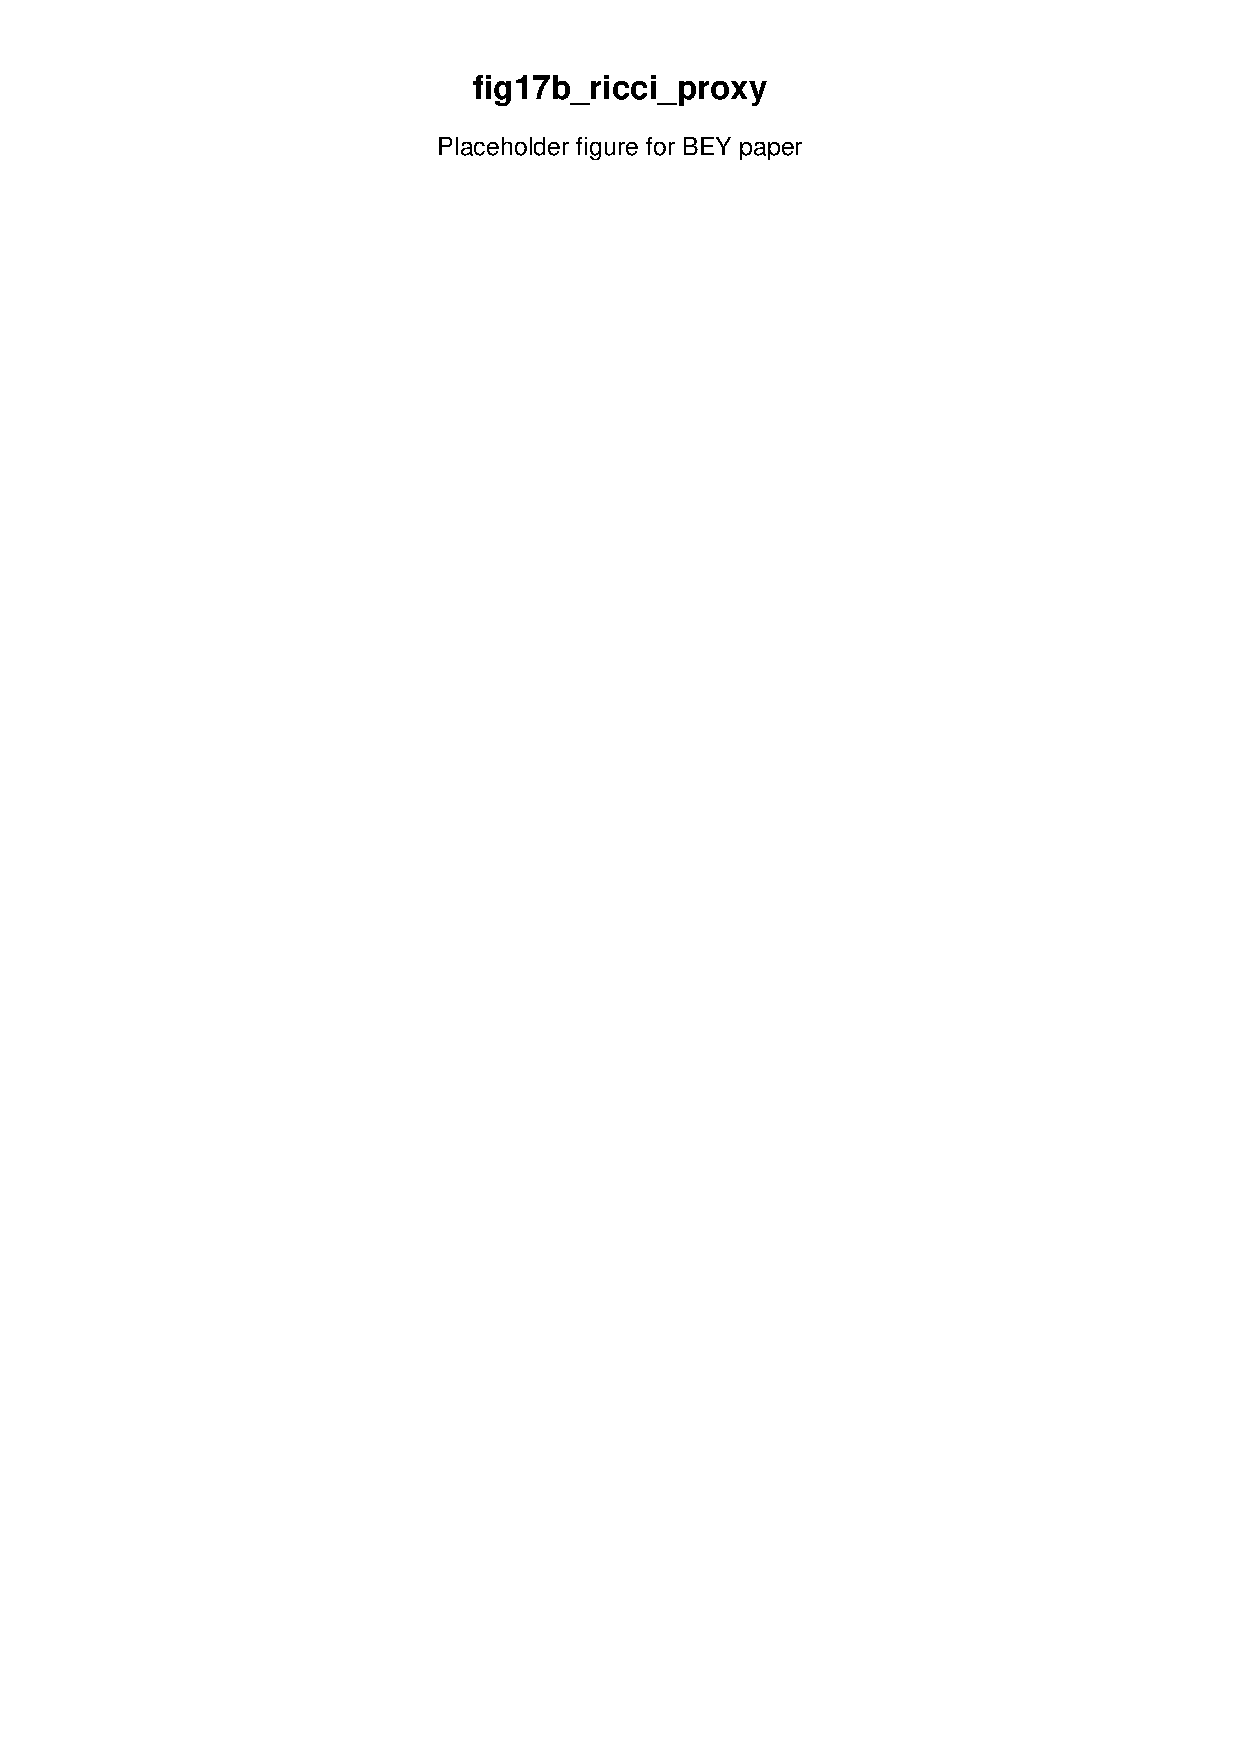
\includegraphics[width=0.48\textwidth]{fig17b_ricci_proxy.pdf}\hfill
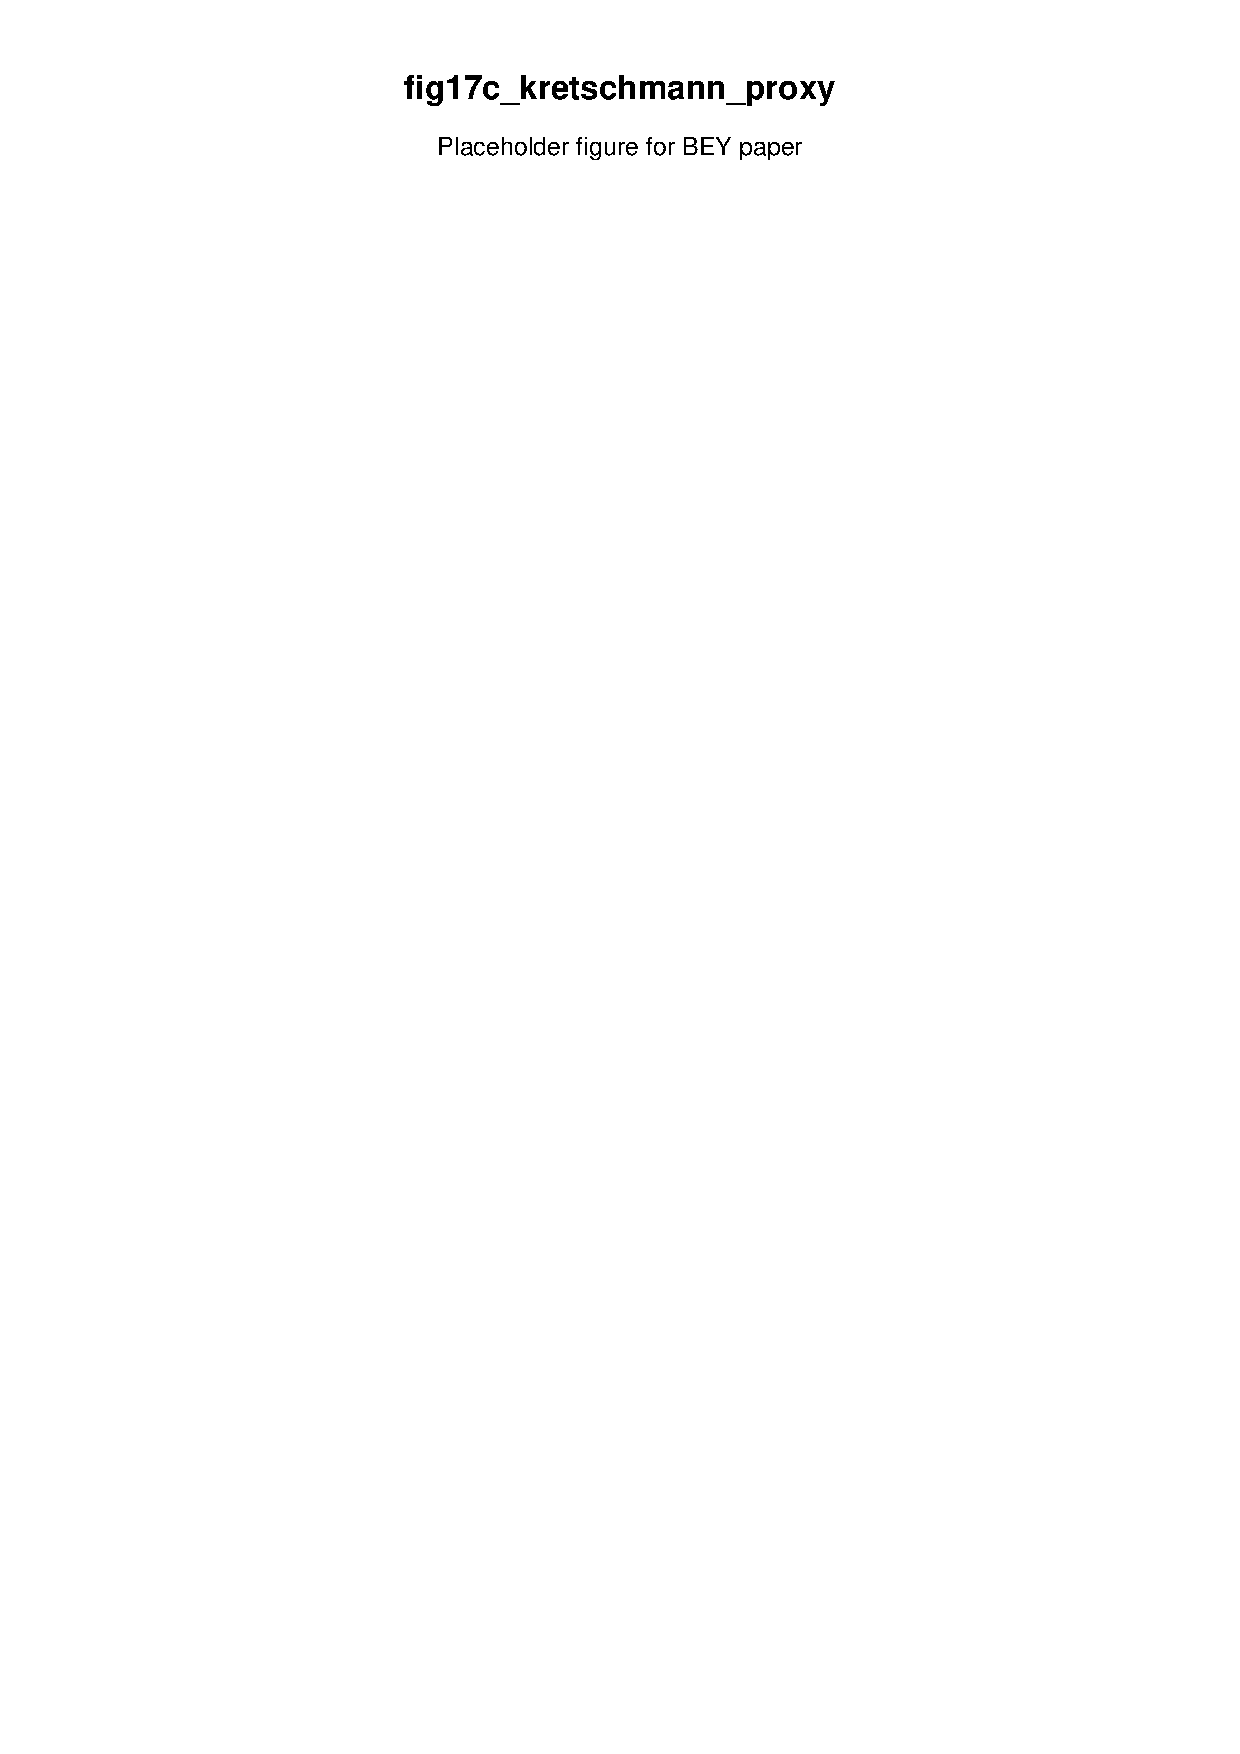
\includegraphics[width=0.48\textwidth]{fig17c_kretschmann_proxy.pdf}
\caption{Curvature diagnostics for the tapered regular-core branch. The Ricci-scalar proxy and Kretschmann-like proxy remain finite across the scanned regularized domain. These plots are regularity diagnostics of the effective ansatz, not a complete quantum-gravity singularity theorem.}
\label{fig:curvature_regular_core}
\end{figure*}

Finally, we map the dimensionless compactness
\begin{equation}
C=\frac{2M}{R_{\rm match}}=A\frac{I(x_m)}{x_m}.
\label{eq:diagnostic_compactness}
\end{equation}
The scan separates four interpretation domains: $C<0.8$ (subcompact),
$0.8<C<0.98$ (compact below horizon), $0.98<C<1$ (conditional horizon-near ECO
branch), and $C\geq1$ (horizon-interior/static-coordinate caution). In the
coarse scan, 44 cases are subcompact, 5 are compact below horizon, no sampled
case falls in the narrow horizon-near ECO bin, and 47 enter the
static-coordinate caution branch. The approximate thresholds for $C\geq1$ are
listed in Table~\ref{tab:compactness_thresholds}. The fiducial branch
$A=1.0$, $x_m=4.0$, $q=2$ remains safely in the $C<1$ domain and is therefore
used only as a clean regular-core diagnostic branch rather than as a full black
hole interior construction.

\begin{table}
\centering
\caption{Approximate $A$ thresholds for the compactness condition $C=2M/R_{\rm match}\geq1$ in the tapered branch.}
\label{tab:compactness_thresholds}
\begin{tabular}{ccc}
\toprule
$x_m$ & $q$ & $A$ threshold for $C\geq1$\\
\midrule
3.0 & 2 & 6.6\\
4.0 & 2 & 7.0\\
5.0 & 2 & 7.6\\
3.0 & 4 & 9.2\\
4.0 & 4 & 8.8\\
5.0 & 4 & 9.2\\
\bottomrule
\end{tabular}
\end{table}

\begin{figure*}
\centering
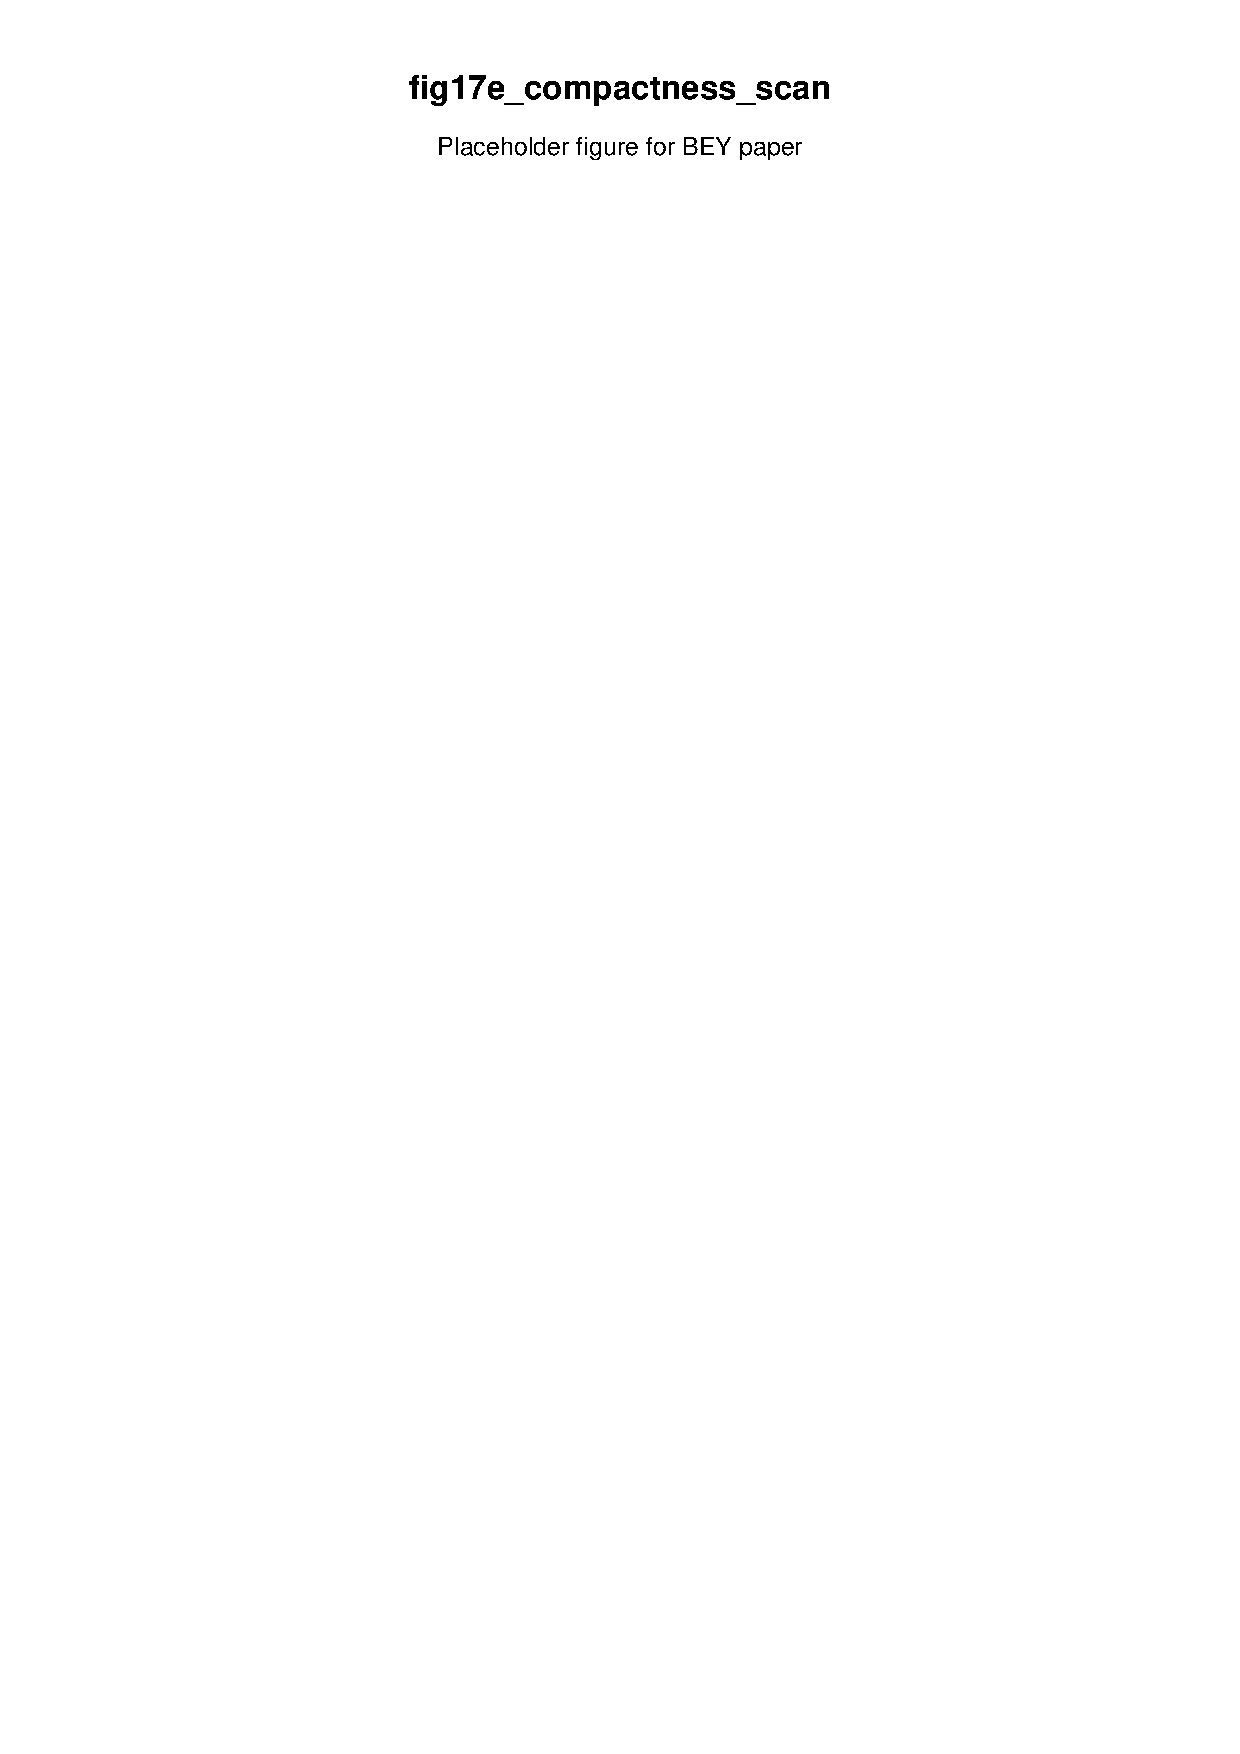
\includegraphics[width=0.48\textwidth]{fig17e_compactness_scan.pdf}\hfill
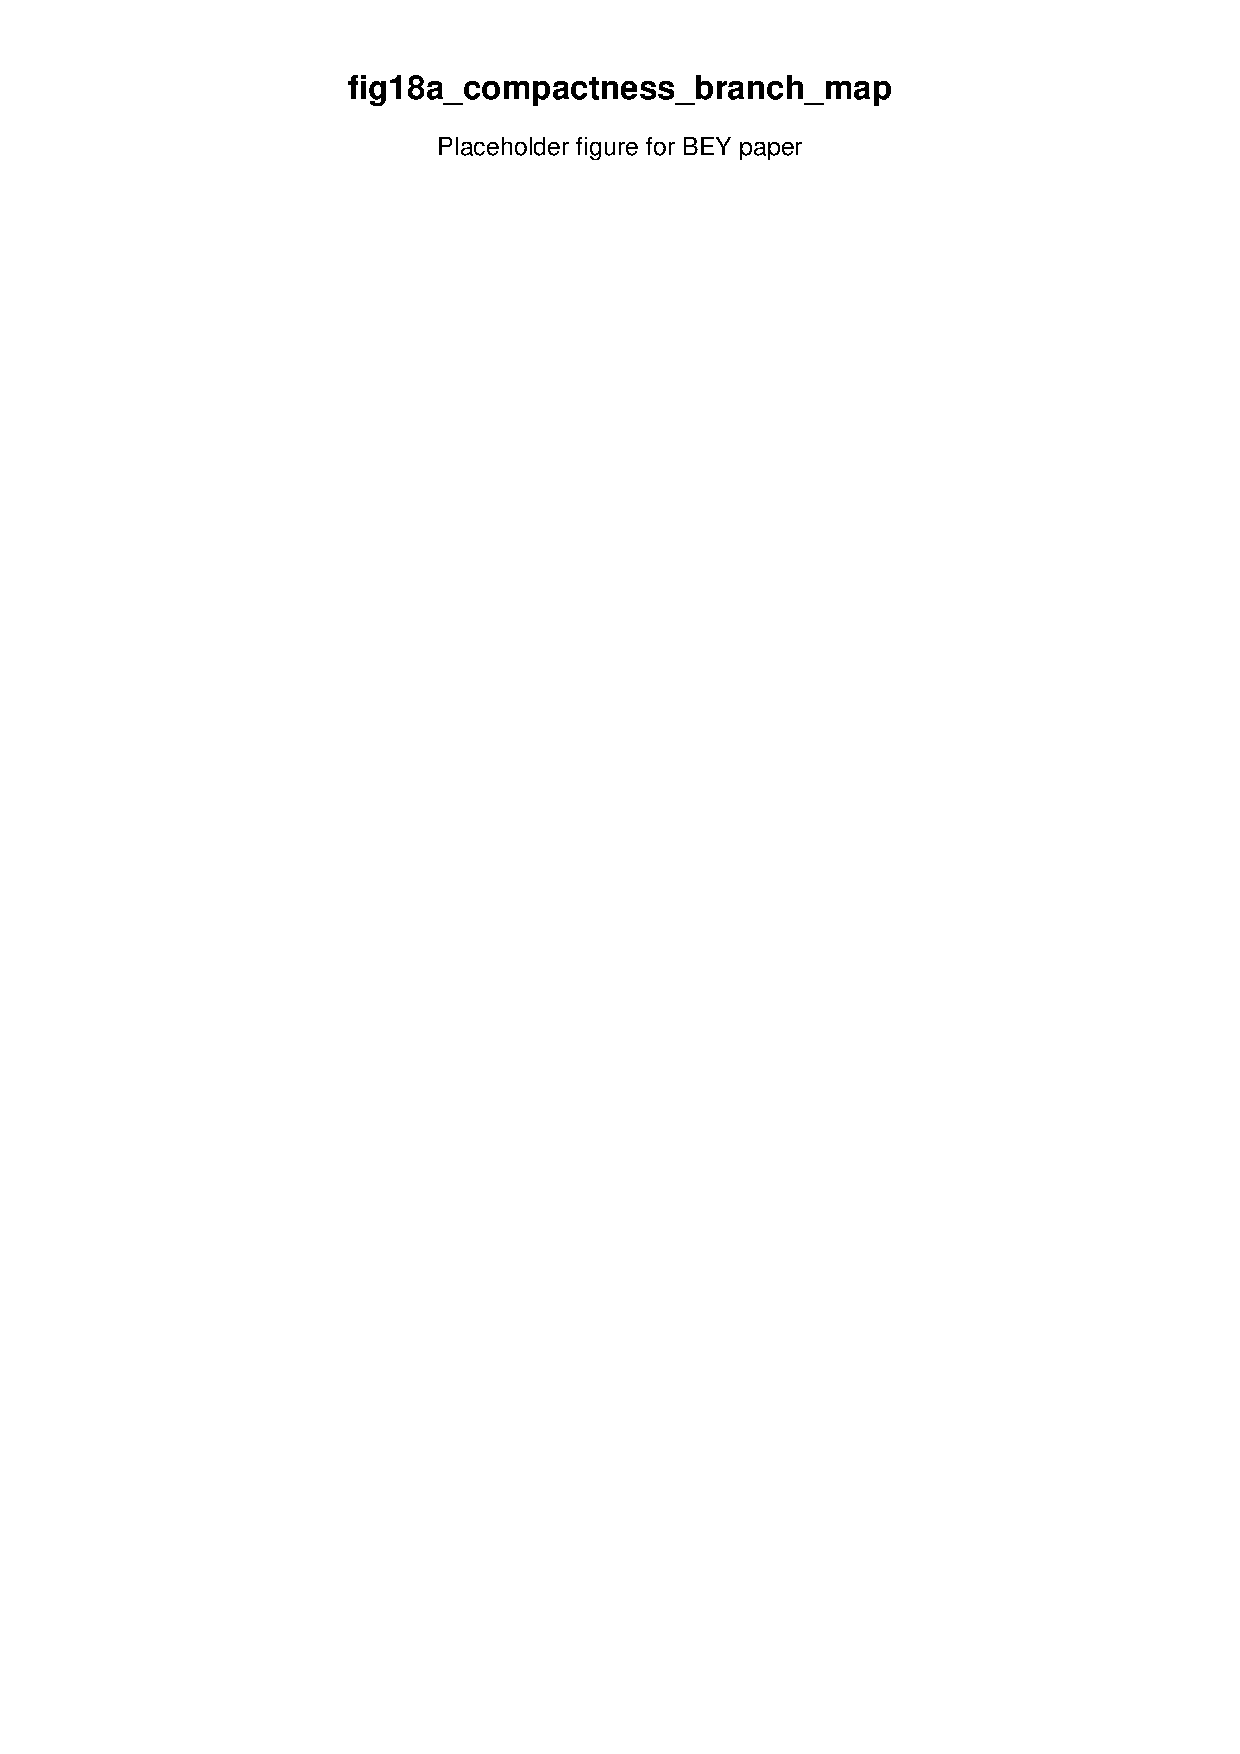
\includegraphics[width=0.48\textwidth]{fig18a_compactness_branch_map.pdf}
\caption{Compactness diagnostics. Left: compactness $C=2M/R_{\rm match}$ as a function of the effective compactness parameter $A$ for the tapered branch. Right: compactness branch map used to distinguish subcompact, horizon-near ECO, and horizon-interior/static-coordinate-caution regions.}
\label{fig:compactness_branch_map}
\end{figure*}

These diagnostics sharpen the scope of the model. The regular-core branch is
well suited for demonstrating finite central density, energy-condition viability
in a broad parameter region, smooth boundary behaviour, and finite curvature
indicators. The horizon-near ECO branch remains a separate phenomenological
channel relevant to echoes. The $C\geq1$ region is compatible with the idea of a
regular interior behind a horizon only in a qualitative sense; a static
single-function ansatz is not, by itself, a complete dynamical black-hole
interior solution.


\subsection{Master diagnostic summary and claim boundaries}
\label{sec:master_diagnostic_summary}

The diagnostic evidence can be collected into a compact claim-safety hierarchy.
The baseline untapered scan demonstrates centre regularity and broad
energy-condition viability, but it leaves a non-zero boundary-pressure diagnostic.
The tapered branch is therefore used as the preferred effective-core branch: it
passes the scanned NEC, WEC, SEC, DEC, centre-regularity, and boundary-softness
filters in all 288 tested cases, with 240 also passing the strict causal-proxy
filter. The curvature scan further gives finite Ricci-scalar and
Kretschmann-like proxies in all 96 tested metric-profile cases.

\begin{table*}
\centering
\caption{Master diagnostic evidence summary. The table separates evidence that
supports the effective regular-core ansatz from the caveats that prevent
overinterpretation as a full Einstein--QCD or full dynamical black-hole interior
solution.}
\label{tab:master_diagnostic_evidence}
\scriptsize
\begin{tabular}{p{0.25\textwidth}p{0.36\textwidth}p{0.28\textwidth}}
\toprule
Diagnostic layer & Core result & Controlled interpretation\\
\midrule
Untapered energy scan &
NEC/WEC/DEC $=56/60$, SEC $=32/60$ &
Baseline energy-condition diagnostic; boundary pressure remains in the
untapered branch.\\
Tapered boundary scan &
NEC/WEC/SEC/DEC $=288/288$, strict causal-proxy acceptance $=240/288$ &
Preferred effective-core branch; the causal proxy is not a full stability
theorem.\\
Smooth matching comparison &
Mean boundary pressure is reduced from $1.77\times10^{-3}$ to
$1.92\times10^{-10}$; warning count $12/12\to0/12$ &
Tapering reduces boundary-pressure tension, but this is not a complete
Darmois--Israel matching proof.\\
Curvature diagnostics &
Finite curvature proxies $=96/96$, regular-centre proxies $=96/96$ &
Supports finite-curvature regularization at toy-model level.\\
Compactness map &
Subcompact $=44$, compact below horizon $=5$, static-coordinate caution $=47$ &
Separates subcompact, horizon-near, and static-caution branches.\\
\bottomrule
\end{tabular}
\end{table*}

Accordingly, the combined diagnostic pipeline supports SC/BEY as an effective
regular-core singularity-replacement framework at the toy-model level. It does
not constitute a full Einstein--QCD solution, a complete Darmois--Israel matching
construction, or a nonlinear stability theorem. The horizon-near ECO/echo sector
should be read only as a conditional phenomenological branch, not as a mandatory
prediction of the model.


\subsection{Einstein--CFL effective-core solutions}
\label{sec:einstein_cfl_effective_solutions}

As an additional matter-supported check, we solve the static Einstein equations
in TOV form for compact cores sourced by a QCD-inspired CFL/bag effective
equation of state. This calculation is not a first-principles Einstein--QCD
solution; it is an Einstein+EOS effective model used to test whether the
regular-core picture can be supported by relativistic hydrostatic matter
profiles. In geometrized units, the isotropic sequence is governed by
\begin{align}
\frac{dm}{dr}&=4\pi r^2\epsilon,
\label{eq:einstein_cfl_tov_mass}\\
\frac{dp}{dr}&=
-\frac{(\epsilon+p)(m+4\pi r^3p)}{r(r-2m)},
\label{eq:einstein_cfl_tov_pressure}\\
\frac{d\Phi}{dr}&=
\frac{m+4\pi r^3p}{r(r-2m)} .
\label{eq:einstein_cfl_tov_phi}
\end{align}
For the effective dense-matter source we use a linear CFL/bag-inspired
equation of state,
\begin{equation}
p=c_s^2\left(\epsilon-\epsilon_{\rm surf}\right),\qquad
c_s^2=\frac{1}{3},
\label{eq:einstein_cfl_linear_eos}
\end{equation}
where \(\epsilon_{\rm surf}\) is set by the bag scale and an effective CFL
pairing contribution. This EOS should be read as a phenomenological
QCD-inspired closure relation, not as a microscopic derivation of the black-hole
interior.

We also test an anisotropic effective-pressure extension,
\begin{equation}
p_t(r)=p_r(r)+\alpha p_r(r)\frac{r^2}{r^2+R_a^2},
\label{eq:einstein_cfl_anisotropy}
\end{equation}
which vanishes at the centre and grows smoothly through the outer core. The
corresponding radial pressure equation becomes
\begin{equation}
\frac{dp_r}{dr}=
-\frac{(\epsilon+p_r)(m+4\pi r^3p_r)}{r(r-2m)}
+\frac{2(p_t-p_r)}{r}.
\label{eq:einstein_cfl_anisotropic_tov}
\end{equation}
This anisotropic branch is an effective pressure-support diagnostic rather than
a full relativistic QCD transport calculation or a nonlinear stability theorem.

\begin{table*}
\centering
\caption{Einstein--CFL effective-core solution summary. The isotropic branch
solves the TOV system with a QCD-inspired CFL/bag EOS. The anisotropic branch
adds a smooth tangential-pressure channel and checks basic energy-condition
compatibility.}
\label{tab:einstein_cfl_effective_summary}
\scriptsize
\begin{tabular}{p{0.27\textwidth}p{0.18\textwidth}p{0.18\textwidth}p{0.27\textwidth}}
\toprule
Branch & Successful solutions & Maximum mass / compactness & Interpretation\\
\midrule
Einstein + QCD-inspired EOS/TOV &
114 &
\(M_{\max}\simeq2.331\,M_\odot\), \(C_{\max}\simeq0.561\) &
Matter-supported compact-core sequence; not a full first-principles
Einstein--QCD solution.\\
Anisotropic Einstein--CFL effective pressure &
222 &
\(M_{\max}\simeq1.950\,M_\odot\), \(C_{\max}\simeq0.579\) &
Tangential pressure-support diagnostic; NEC/SEC/DEC passed in all successful
solutions of the scanned grid.\\
\bottomrule
\end{tabular}
\end{table*}

The isotropic scan reaches \(M_{\max}\simeq2.331\,M_\odot\) at
\(R\simeq12.75\,{\rm km}\), while the anisotropic scan reaches
\(M_{\max}\simeq1.950\,M_\odot\) at \(R\simeq10.275\,{\rm km}\). Both branches
remain horizon-exterior in the present implementation. This is useful
conservative evidence: the calculation strengthens the matter-supported side of
the SC/BEY programme without converting the proposal into a claimed complete
black-hole interior solution.

\begin{figure*}
\centering
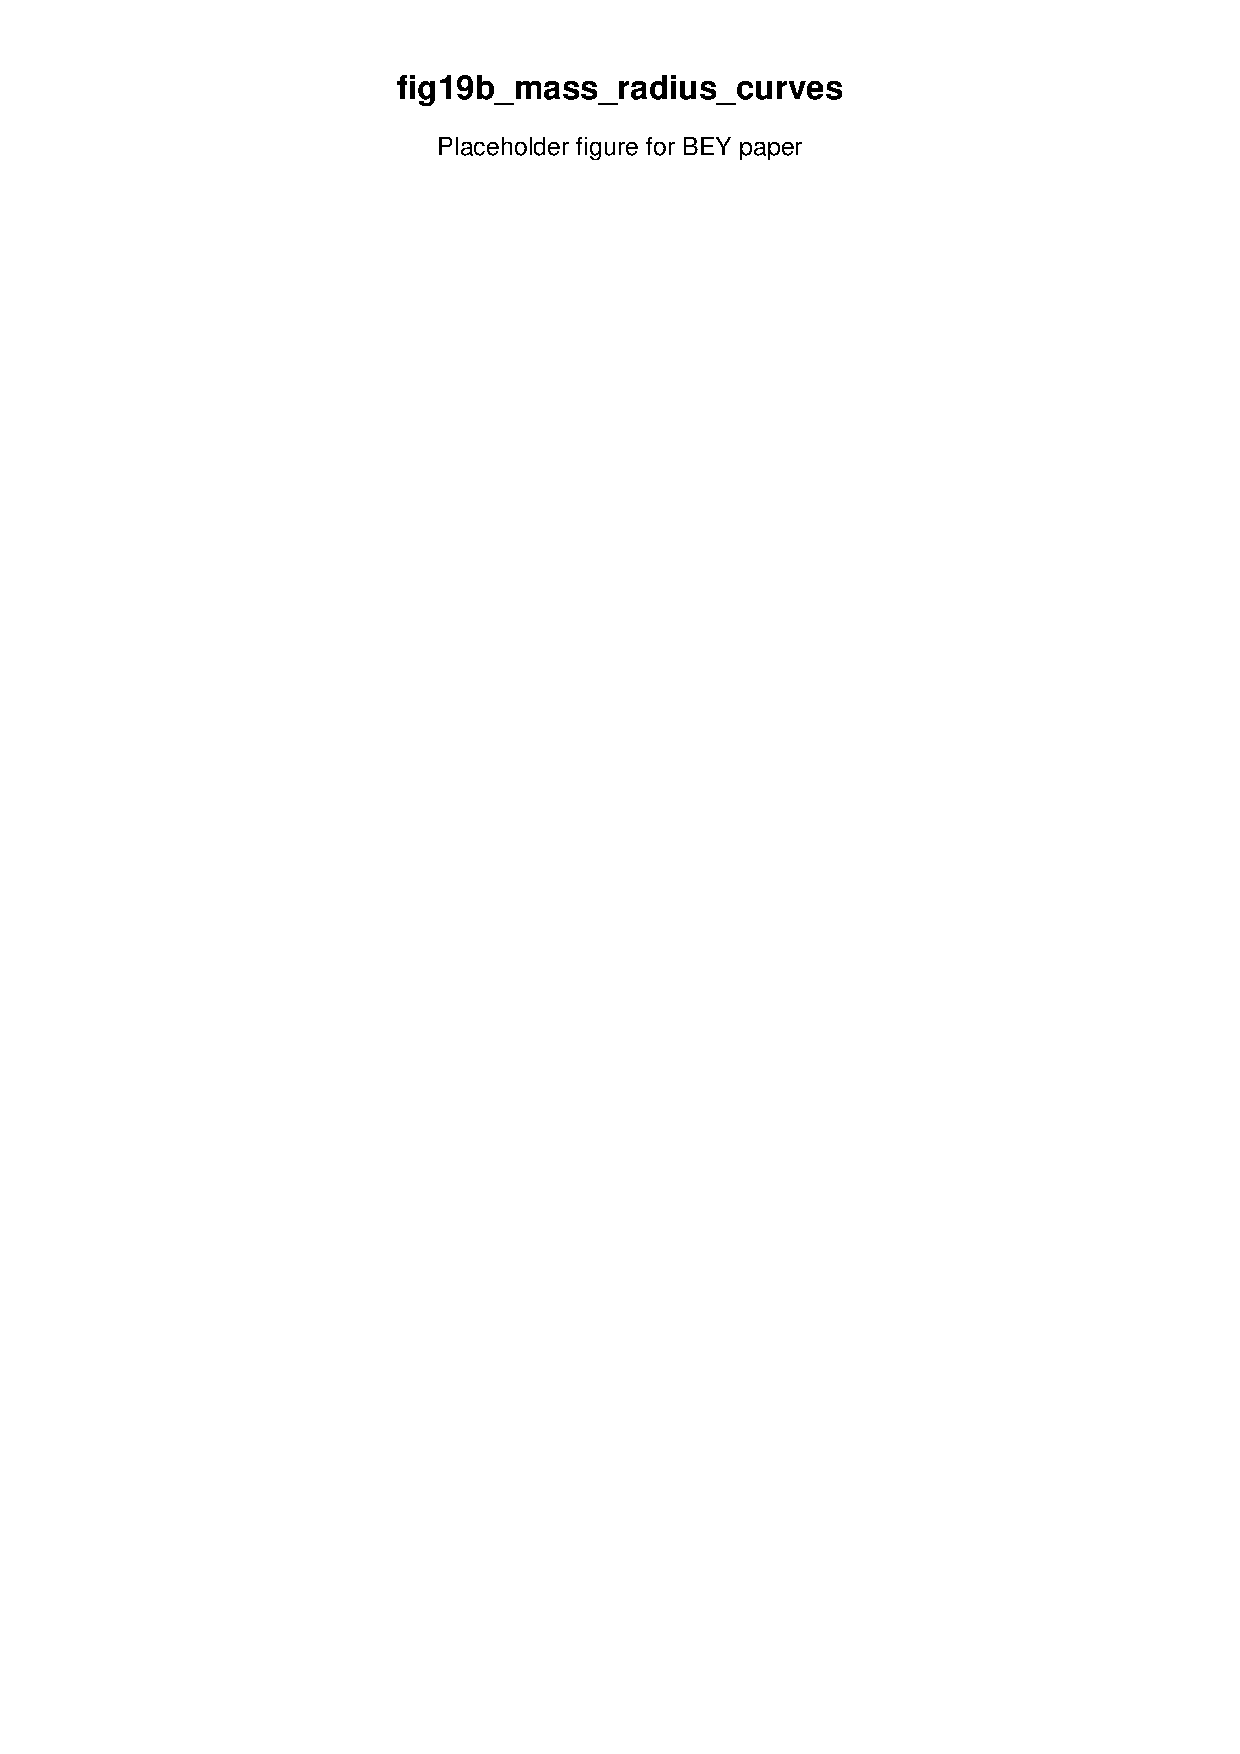
\includegraphics[width=0.48\textwidth]{fig19b_mass_radius_curves.pdf}
\hfill
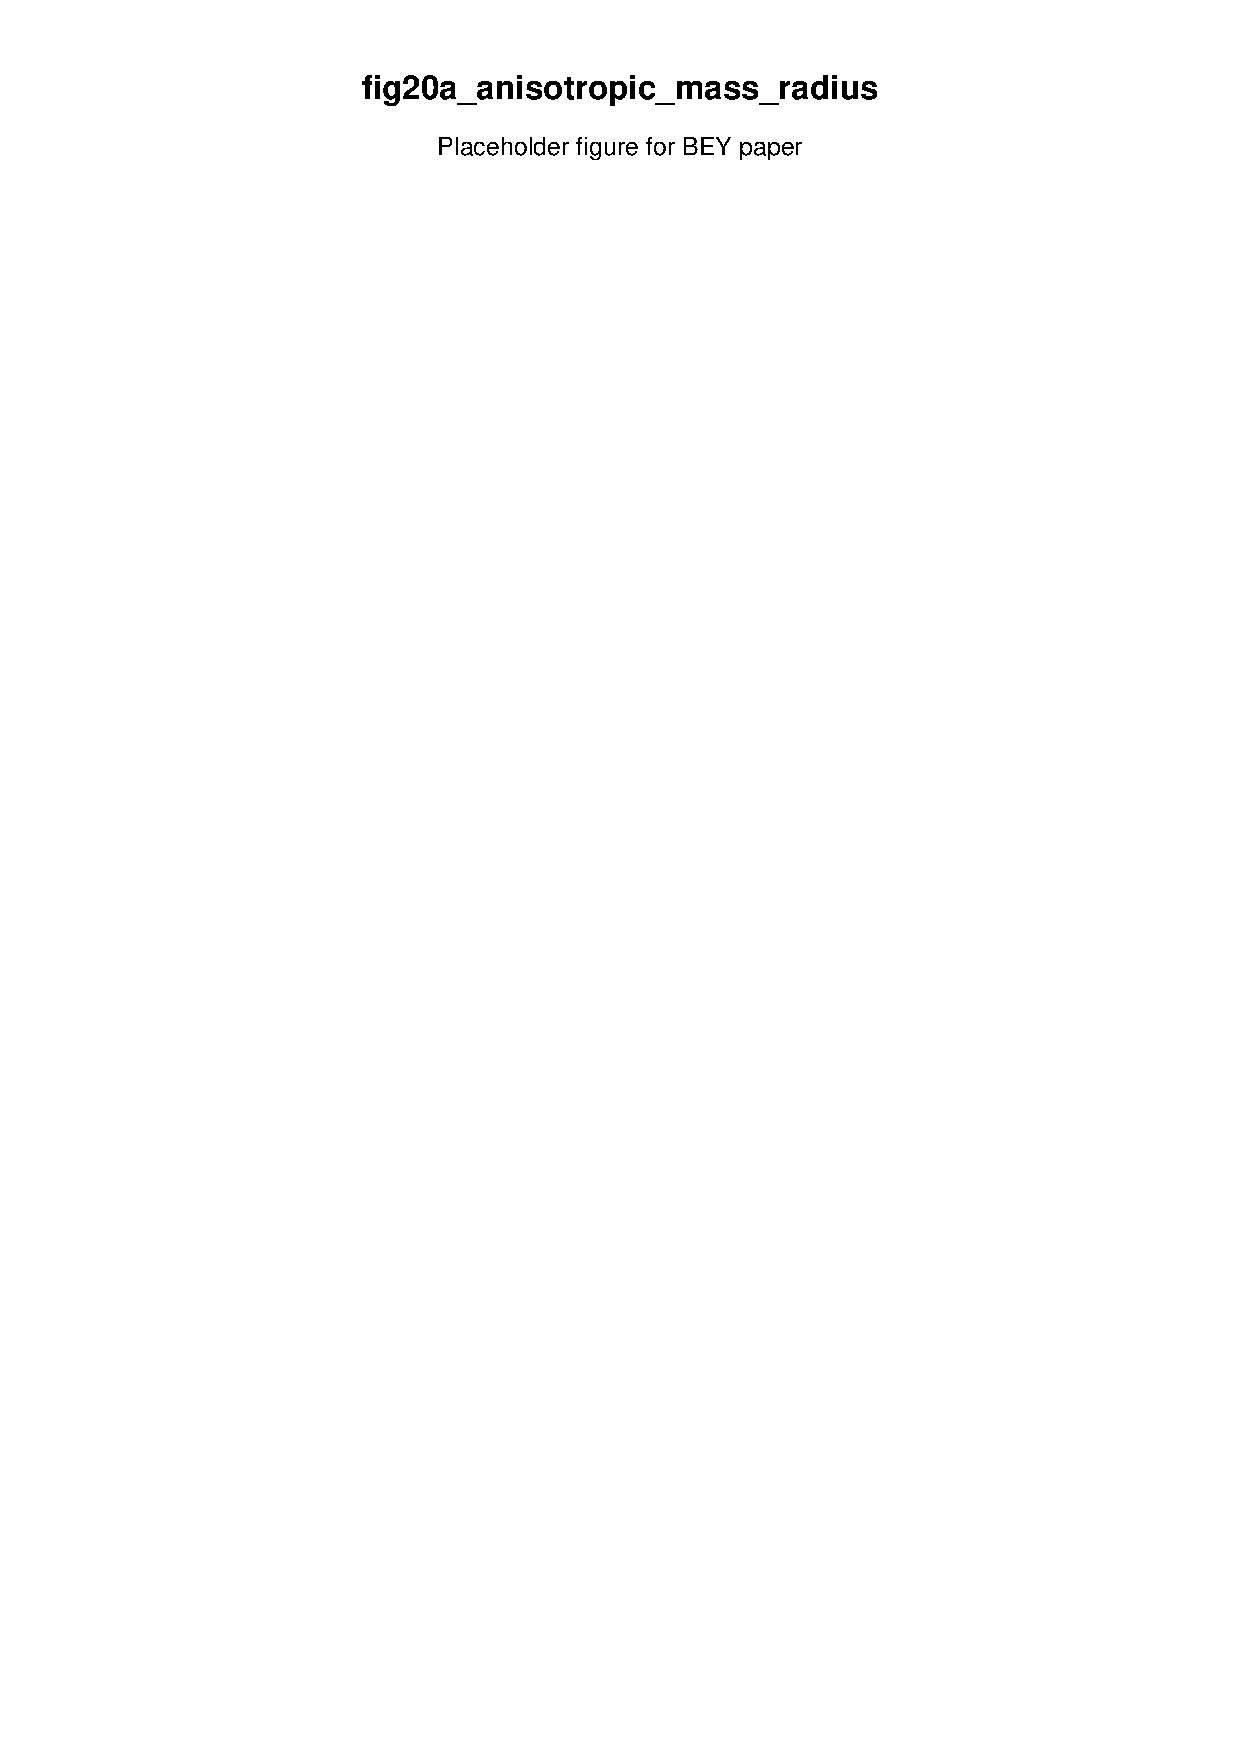
\includegraphics[width=0.48\textwidth]{fig20a_anisotropic_mass_radius.pdf}
\caption{Einstein--CFL effective-core mass--radius diagnostics. Left:
isotropic TOV sequences sourced by QCD-inspired CFL/bag effective equations of
state. Right: anisotropic effective-pressure sequences for different
anisotropy strengths \(\alpha\).}
\label{fig:einstein_cfl_mass_radius}
\end{figure*}

\begin{figure*}
\centering
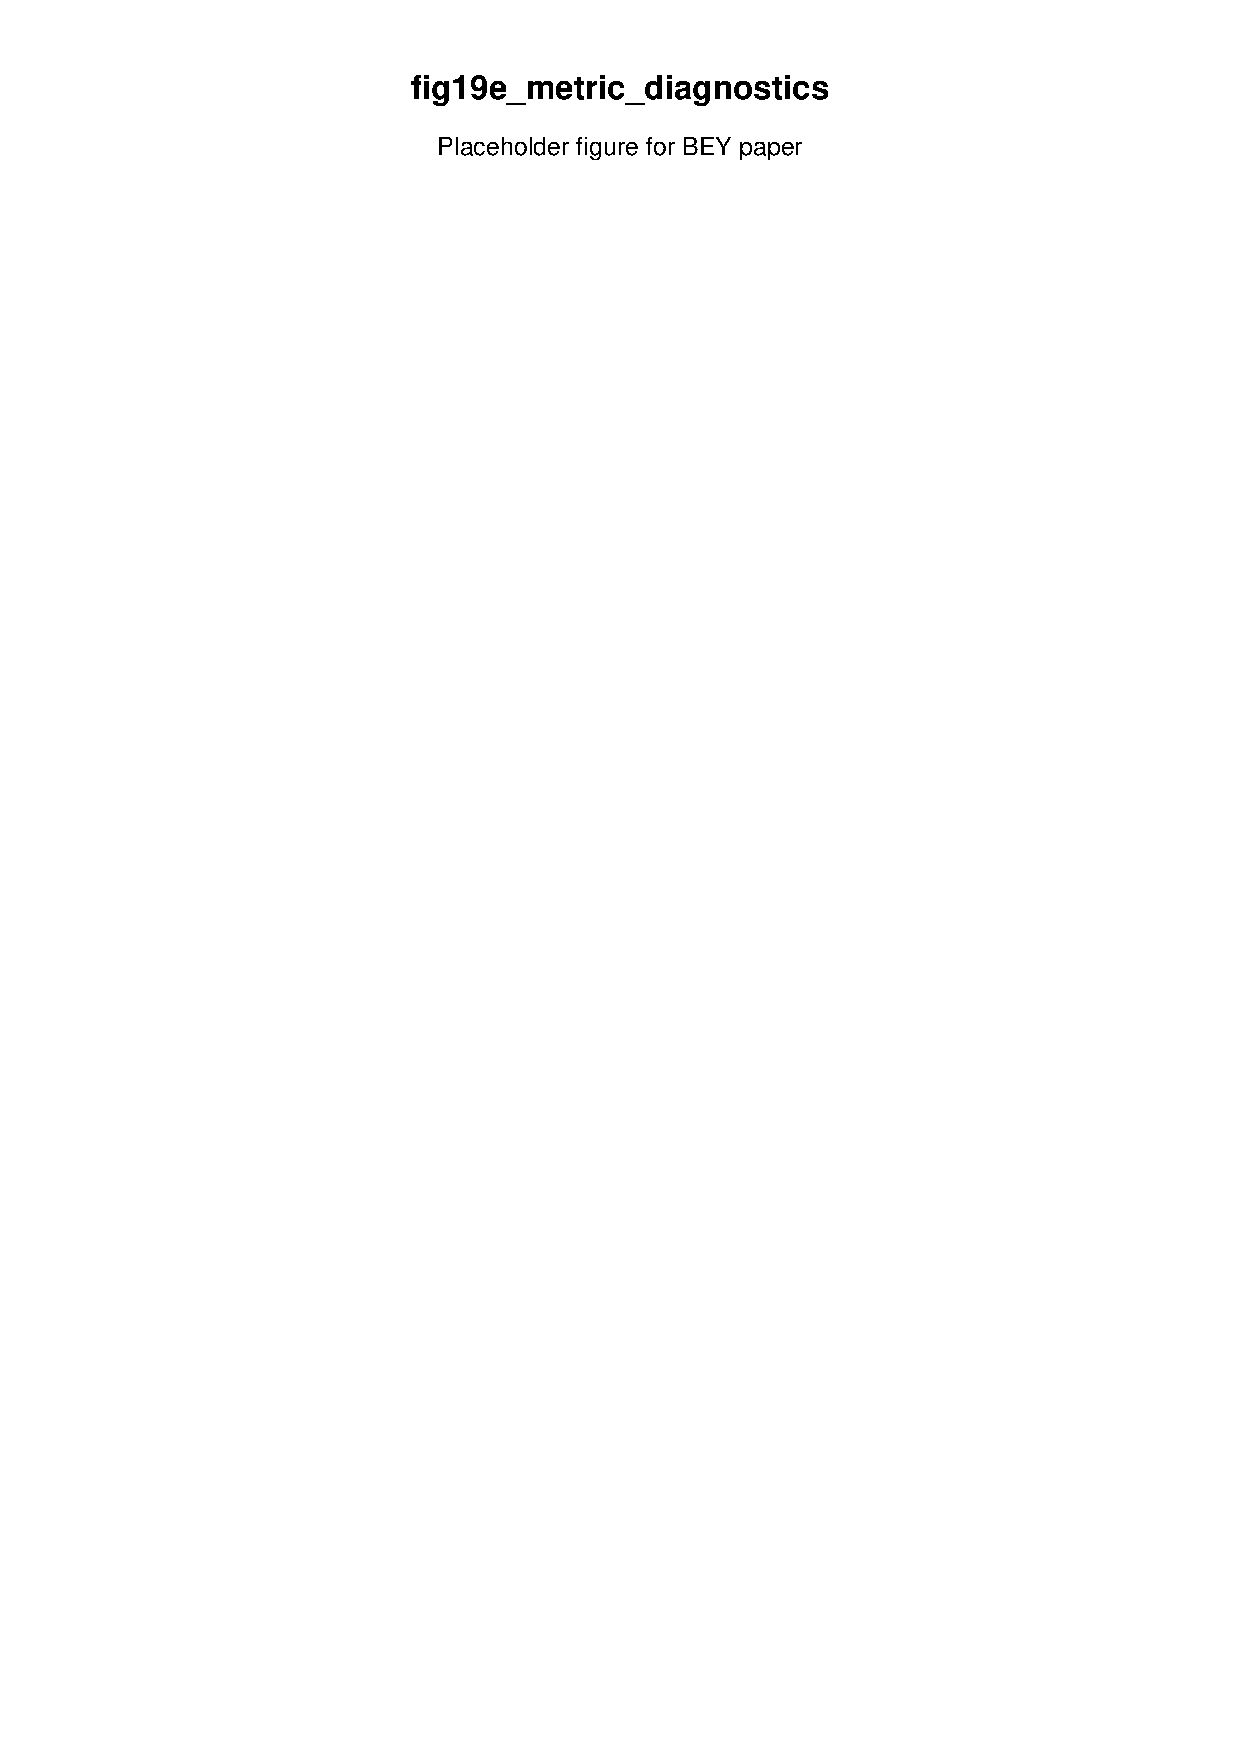
\includegraphics[width=0.48\textwidth]{fig19e_metric_diagnostics.pdf}
\hfill
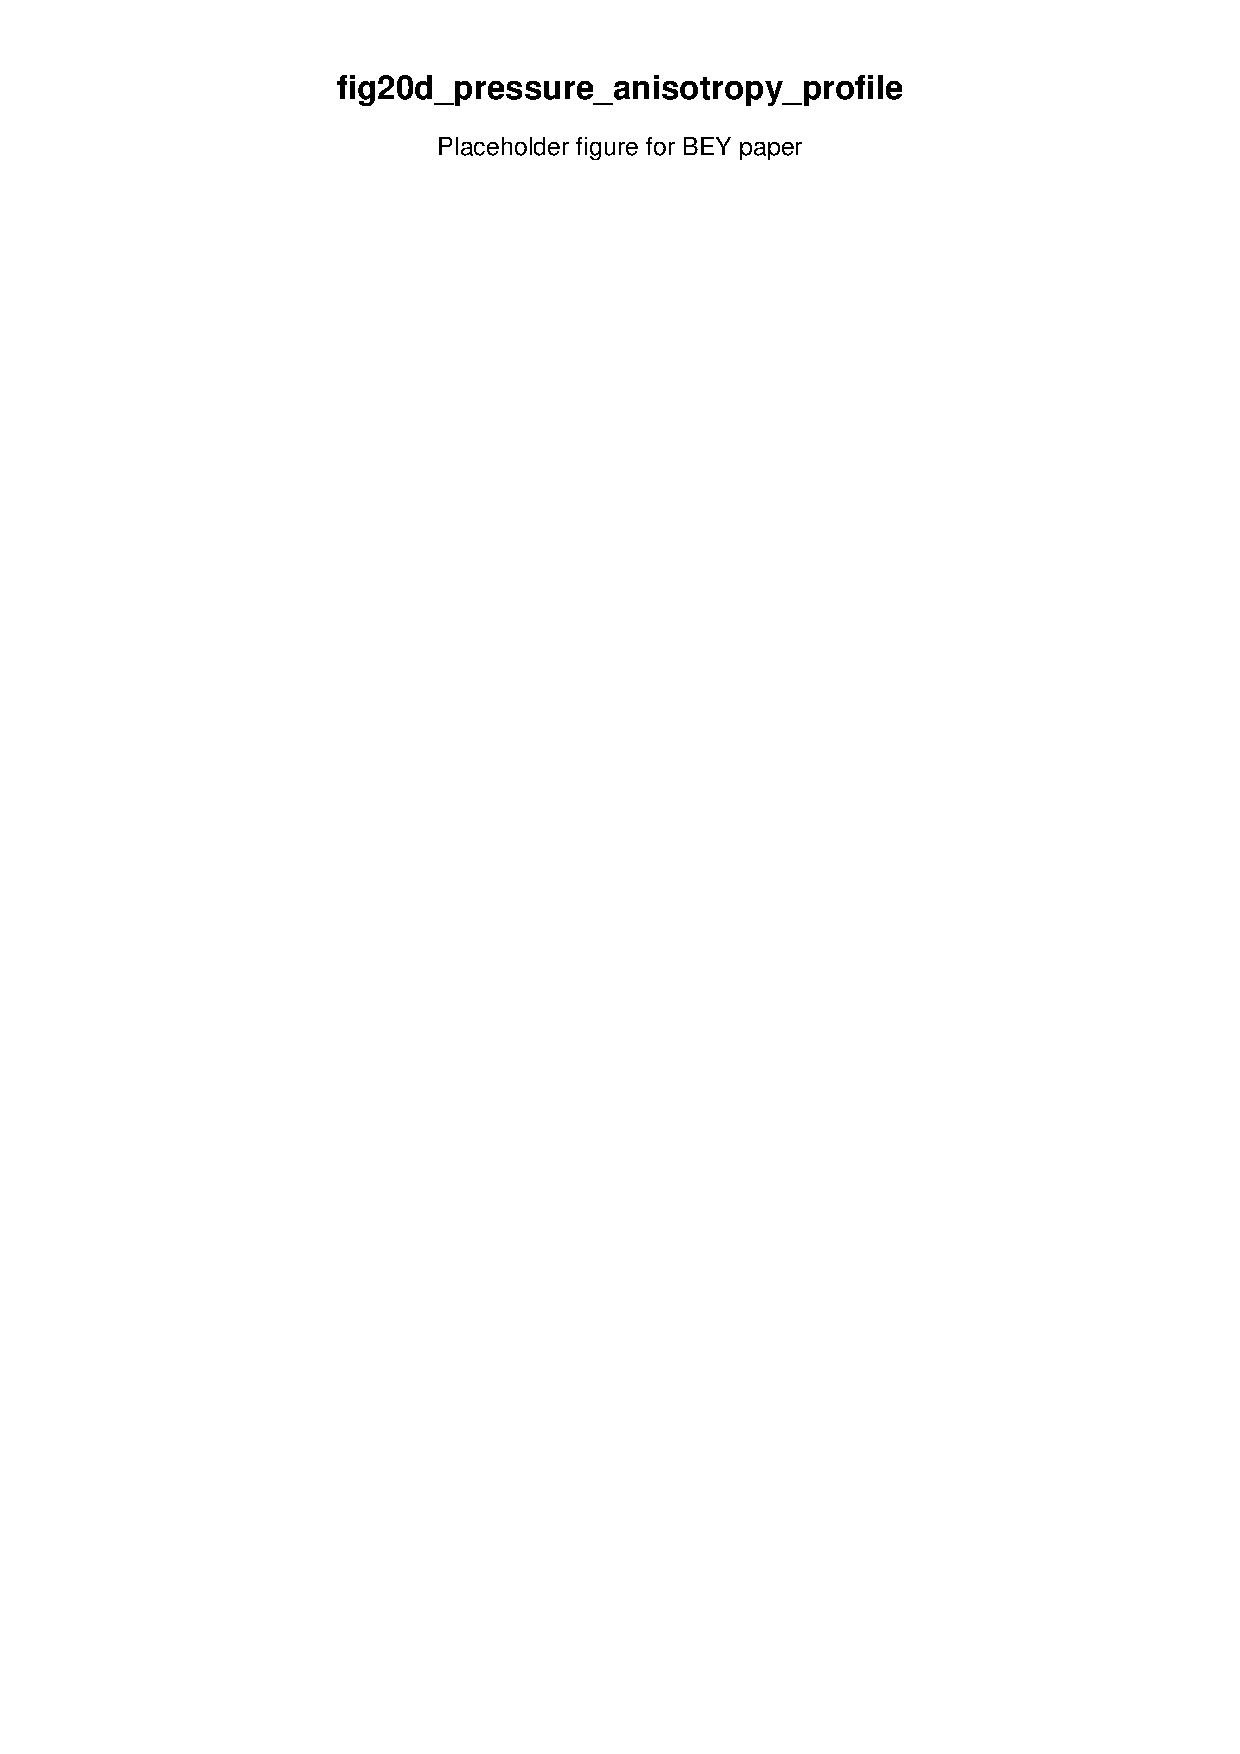
\includegraphics[width=0.48\textwidth]{fig20d_pressure_anisotropy_profile.pdf}
\caption{Representative Einstein--CFL effective-core profiles. Left:
metric-function diagnostics for a representative isotropic TOV solution. Right:
radial, tangential, and anisotropic pressure profiles for a representative
anisotropic CFL effective-core solution.}
\label{fig:einstein_cfl_representative_profiles}
\end{figure*}


%============================================================
\section{Robustness Under Rotation: Kerr Extension}
\label{sec:kerr}

The majority of astrophysical black holes carry significant angular momentum. We extend the analysis to slowly rotating (Kerr) backgrounds using simple compactness estimates. For a Kerr black hole of mass $M$ and spin $a_*$, the outer horizon $r_+(a_*) = (GM/c^2)(1 + \sqrt{1-a_*^2})$ is smaller than $R_s$, so the mean density inside the horizon increases with spin. To leading order: $\bar\rho(a_*) \approx \bar\rho_0(1 + \tfrac{3}{4}a_*^2)$, and $\mu_q(a_*) \approx \mu_q(0)(1 + \tfrac{1}{4}a_*^2)$.

\begin{table}
\caption{Compactness-estimate Kerr extension for $M = 60\,M_\odot$.}
\label{tab:kerr}
\begin{tabular}{ccccc}
\hline\noalign{\smallskip}
$a_*$ & $r_+$ [km] & $\bar\rho$ [kg/m$^3$] & $\mu_q$ [MeV] & Deconf.\ ? \\
\noalign{\smallskip}\hline\noalign{\smallskip}
0.00 & 177.2 & $5.12\times10^{15}$ & 314.6 & Yes \\
0.30 & 173.2 & $5.49\times10^{15}$ & 314.6 & Yes \\
0.50 & 165.4 & $6.30\times10^{15}$ & 314.8 & Yes \\
0.70 & 151.9 & $8.13\times10^{15}$ & 315.1 & Yes \\
0.90 & 127.2 & $1.38\times10^{16}$ & 315.9 & Yes \\
0.99 & 101.1 & $2.76\times10^{16}$ & 317.4 & Yes \\
\noalign{\smallskip}\hline
\end{tabular}
\end{table}

\paragraph{Physical interpretation.}
Simple compactness estimates suggest that rotation does not obviously invalidate the condensation scenario. For $a_* \to 1$ (near-extremal Kerr), the inner horizon approaches the outer horizon; the SC core would then be confined to a smaller volume, further increasing the local density. We emphasise that the notion of ``horizon volume'' in Kerr is coordinate-dependent, and a complete treatment requires solving the condensate equations in oblate-spheroidal coordinates with frame-dragging effects included.

\begin{figure*}
\resizebox{0.92\textwidth}{!}{%
  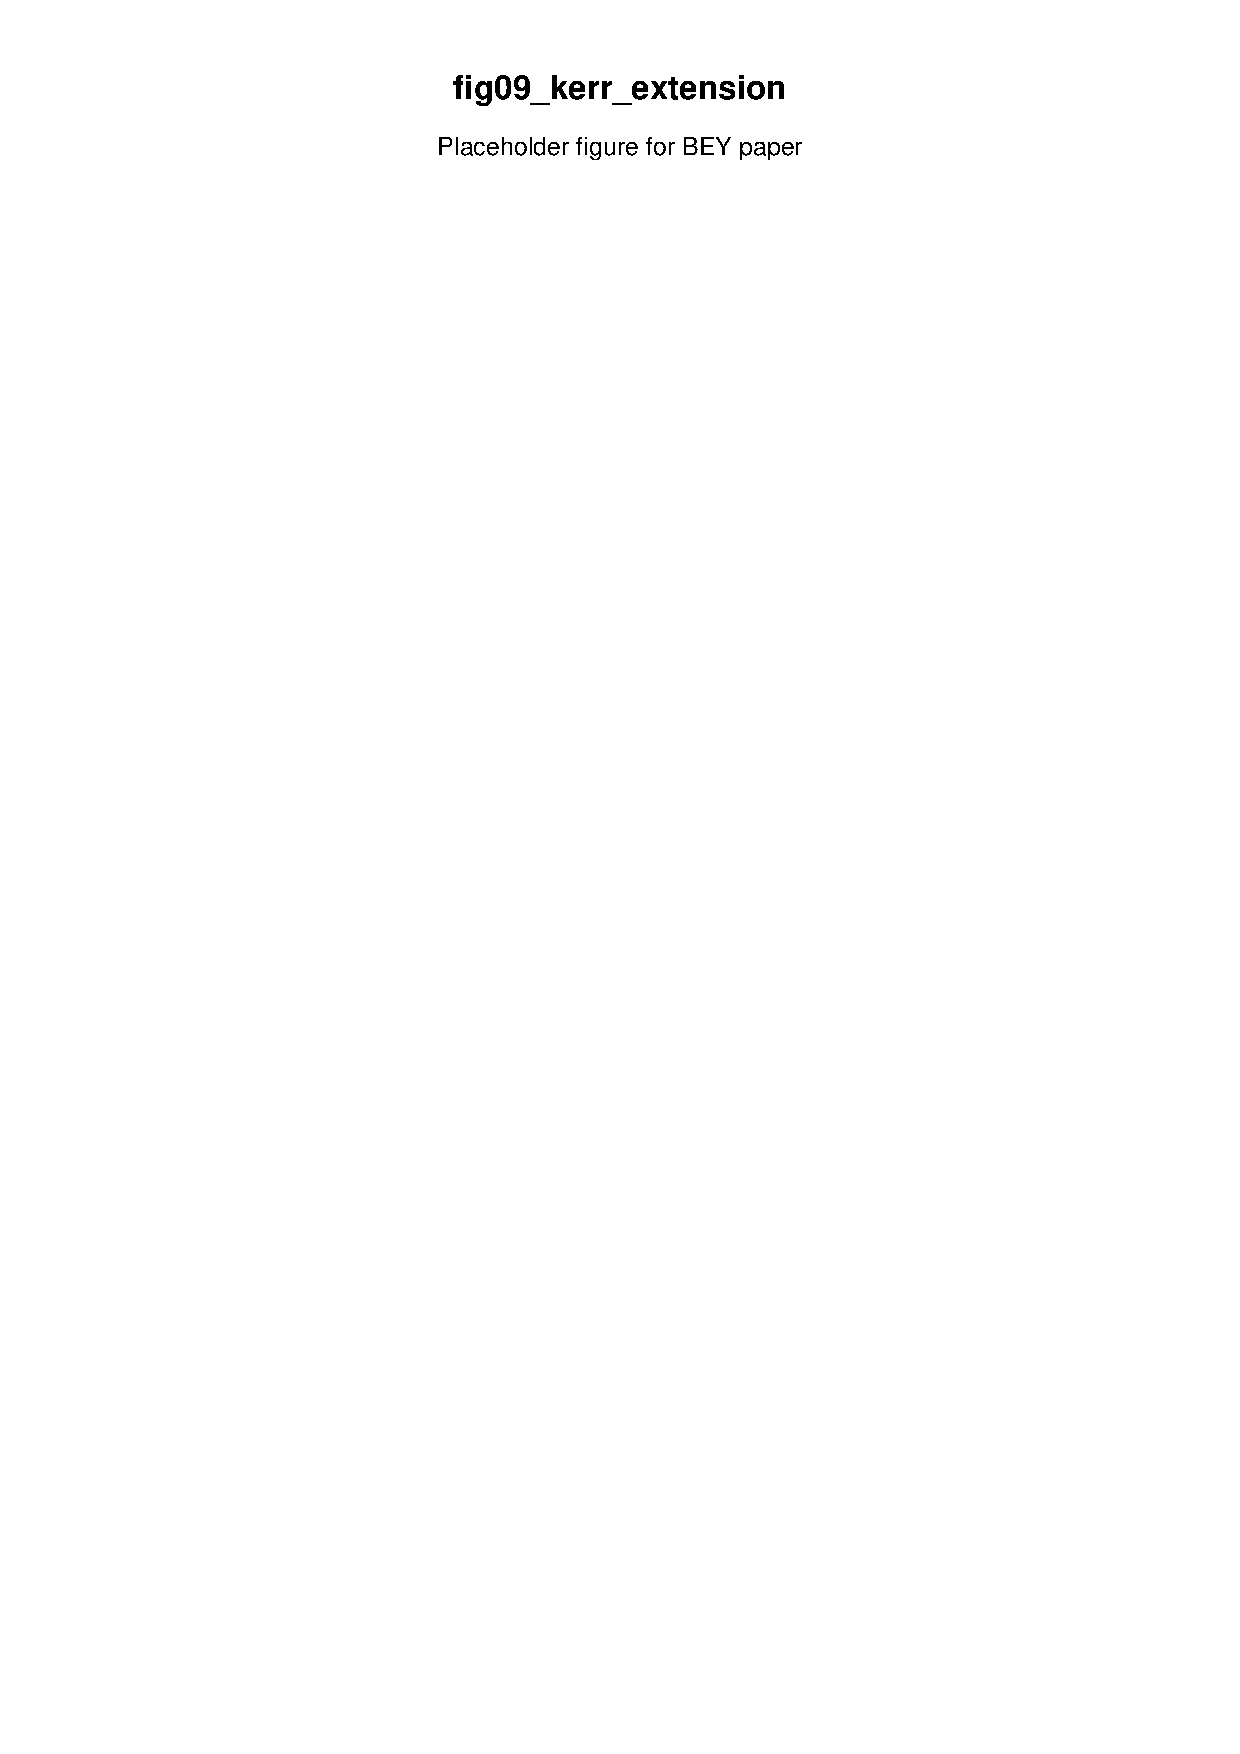
\includegraphics{fig09_kerr_extension.pdf}
}
\caption{Compactness-estimate Kerr extension. \textbf{Left:} $r_+/R_s$ and $\bar\rho/\bar\rho_0$ vs.\ spin $a_*$ for $60\,M_\odot$. \textbf{Right:} $\mu_q(a_*)$ remains above the QCD deconfinement scale for all spins.}
\label{fig:kerr}
\end{figure*}

%============================================================
\section{Comparison with Other Non-Singular Models}
\label{sec:comparison}

Schwarzschild Condensation is one of several proposals in the literature for replacing the classical singularity. Table~\ref{tab:comparison} provides a structured comparison.

\begin{table*}
\caption{Comparison of Schwarzschild Condensation with other non-singular black-hole and compact-object models.}
\label{tab:comparison}
\begin{tabular}{lccccc}
\hline\noalign{\smallskip}
Model & Interior & Matching & Stability & Echoes & Microphysics \\
\noalign{\smallskip}\hline\noalign{\smallskip}
Classical Schwarzschild & Vacuum, singular & N/A & N/A & No & --- \\
Bardeen (1968) \cite{Bardeen1968}    & Magnetic monopole & Smooth & Partial & No & Magnetic source \\
Hayward (2006) \cite{Hayward2006}    & Effective fluid & Smooth & Partial & No & Effective EOS \\
Dymnikova (1992) \cite{Dymnikova1992}    & de Sitter, vacuum & Smooth & Partial & No & Vacuum polar. \\
Gravastar \cite{MazurMottola2004,Visser2004} & dS + thin shell & Thin shell & Yes & Yes (ECO) & Vacuum condensate \\
Boson star \cite{Kaup1968,Ruffini1969,LieblingPalenzuela2017} & Scalar BEC, no horizon & N/A & Yes (some) & Yes & Fund.\ scalar \\
Dvali-Gomez \cite{DvaliGomez2013} & Graviton condensate & At horizon & Critical & --- & Graviton self-int. \\
\textbf{SC (this work)} & QCD cond.\ + dS & Thin shell & Yes (BdG) & Yes ($\sim$8 ms) & Color SC \\
\noalign{\smallskip}\hline
\end{tabular}
\end{table*}

The distinguishing features of SC are: (i) a concrete QCD microphysical foundation (color superconductivity, neutron-star phenomenology); (ii) intermediate position between gravastars (vacuum-energy) and boson stars (fundamental scalar)---the condensing degrees of freedom are composite Cooper pairs; (iii) quantitative kinetic check (Sect.~\ref{sec:kinetics}); (iv) specific frequency-shift signature in the ECO echo channel tied to QCD physics.

%============================================================
\section{Cosmological Outlook}
\label{sec:cosmology}

The mathematical structure of bounded-density regular interiors finds parallel applications in singularity-free cosmology, where the Big Bang singularity is replaced by a bounce. In a spatially flat FRW universe with bounded energy density $\epsilon(a) = \epsilon_c/[1 + (a_b/a)^4]$, the Friedmann equation $H^2 = (8\pi G/3)\epsilon$ admits a minimum scale factor $a_{\min} \sim a_b$. The structural analogy with the SC core (bounded $\epsilon \leq \epsilon_0$) suggests a unified perspective on singularity resolution. We note that this is a structural analogy at the level of mathematical form, not a derivation that the same microphysics operates in both regimes; the cosmological application would require dedicated analysis.

%============================================================
\section{Information Paradox and Entropy Estimate}
\label{sec:information}

\subsection{Geometric obstacle to unitarity}
\label{sec:geom_obstacle}

The classical singularity acts as a spacelike boundary on which Cauchy surfaces terminate \cite{Hawking1975,Preskill1992,Page1993}, and the interior Hilbert space is not well-defined as a function of time. In Schwarzschild Condensation, the regular interior would remove this geometric obstacle within the effective model. Cauchy surfaces extend smoothly; $\mathcal{H}_{\rm in}$ would have a well-defined dimension at all times. We emphasise: this does not by itself derive the Page curve or prove unitary evaporation. It removes the singular geometric obstruction; the explicit mapping between interior condensate modes and exterior Hawking radiation remains an open problem.

\subsection{Hilbert space dimension and entropy estimate}
\label{sec:entropy}

The condensate excitation modes are the 3D harmonic-oscillator modes of the de Sitter trap with energies $E_{n\ell m} = \hbar\omega(2n + \ell + 3/2)$. The number of modes below the natural UV cutoff scales as
\begin{equation}
\dim\mathcal{H}_{\rm in} \sim (R_s/\sigma)^3 \sim (M/m_{\rm pair})^{3/2},
\label{eq:dim_H}
\end{equation}
giving $\dim\mathcal{H}_{\rm in} \sim 10^{26}$ for $M = 1\,M_\odot$ and $S_{\rm SC}/k_B \sim 60$. The Bekenstein-Hawking entropy $S_{\rm BH}/k_B \sim 10^{77}$ is many orders larger; the ratio scales as $S_{\rm SC}/S_{\rm BH} \propto M^{-1/2}$.

\paragraph{Physical interpretation.}
This estimate is order-of-magnitude only. The disparity $S_{\rm SC} \ll S_{\rm BH}$ is consistent with holographic and membrane-paradigm pictures: $S_{\rm BH}$ is an area law reflecting horizon degrees of freedom, while $S_{\rm SC}$ counts only the bulk condensate modes. SC is therefore not in conflict with the Bekenstein bound.

\begin{figure*}
\resizebox{0.92\textwidth}{!}{%
  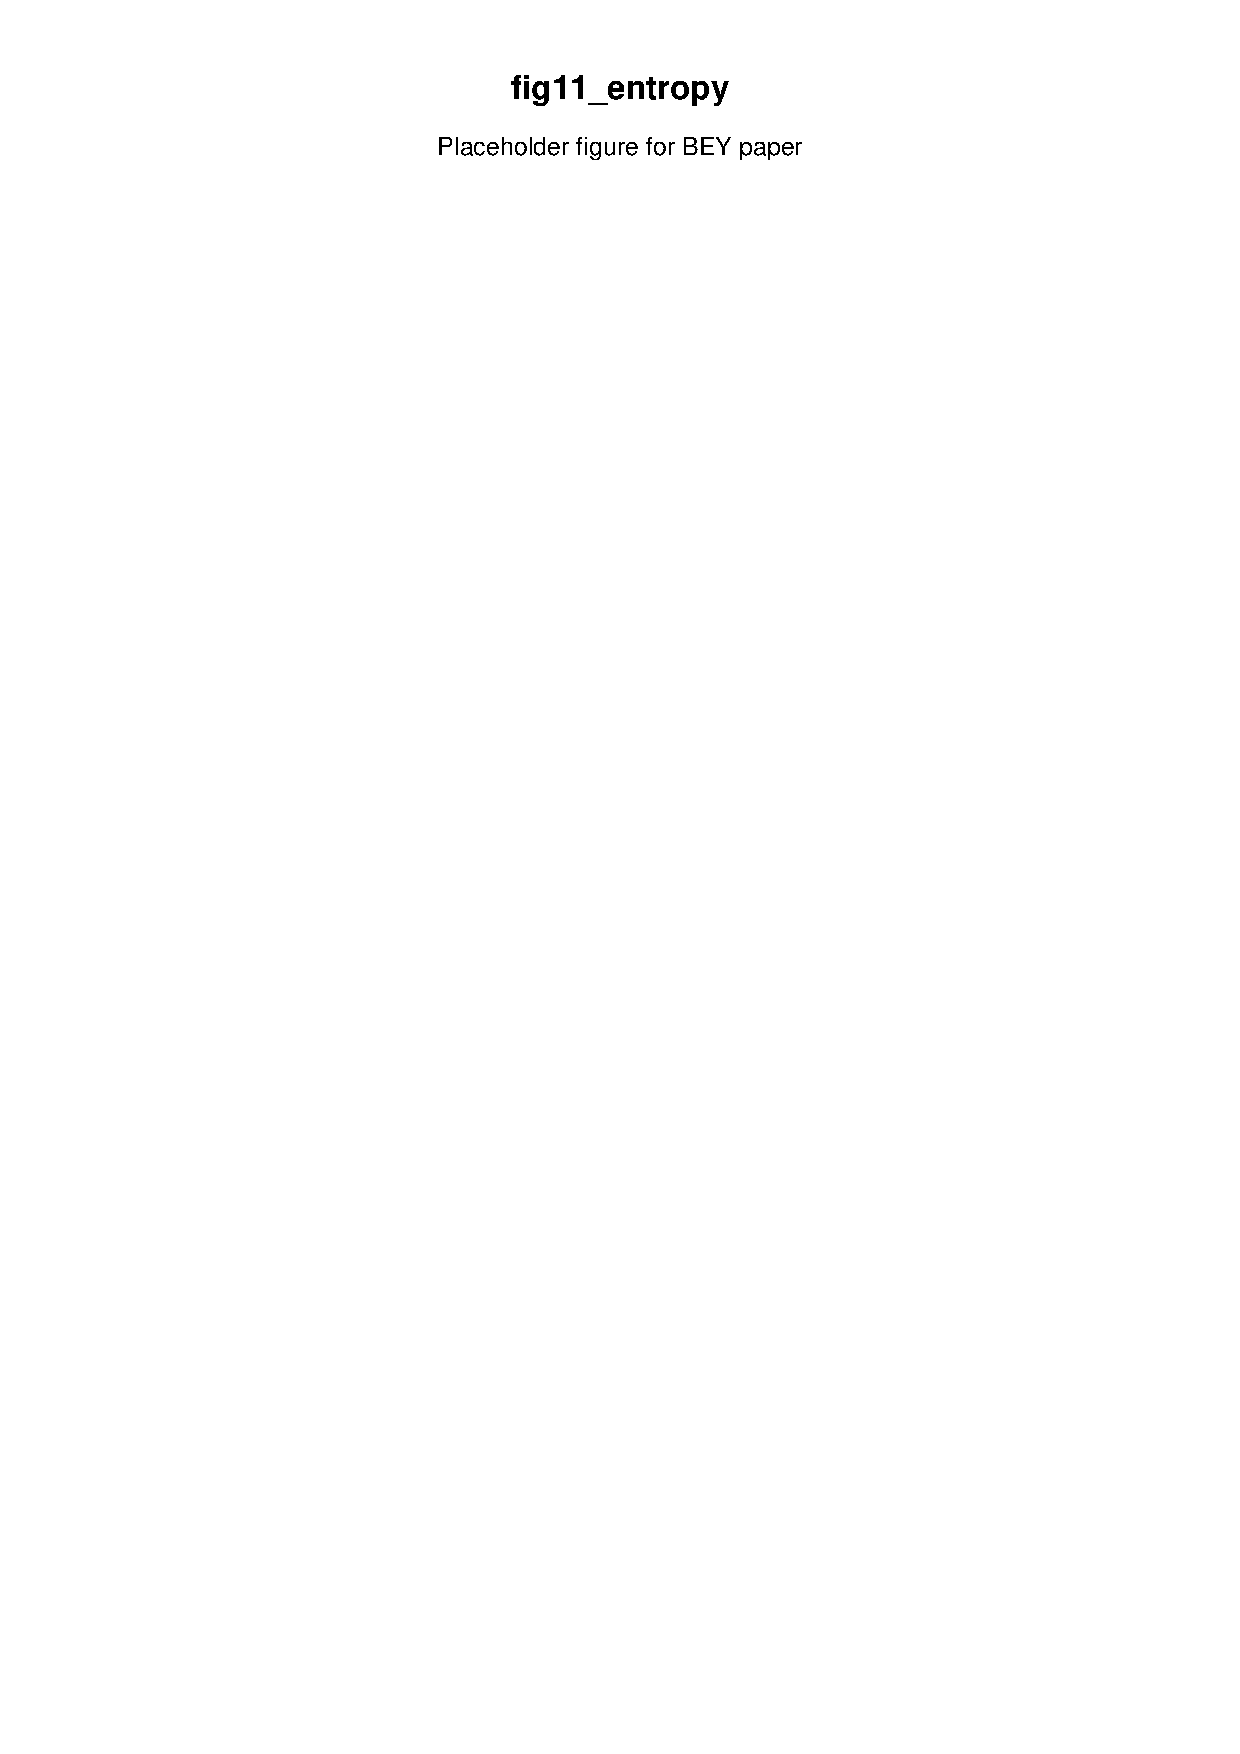
\includegraphics{fig11_entropy.pdf}
}
\caption{Estimate-level entropy of the SC core compared with $S_{\rm BH}$. \textbf{Left:} both as functions of mass. \textbf{Right:} the ratio $S_{\rm SC}/S_{\rm BH}$ is always $\ll 1$, consistent with horizon-dominated black-hole entropy.}
\label{fig:entropy}
\end{figure*}

%============================================================
\section{Observational Predictions and Tests}
\label{sec:observations}

A central question is whether SC-class regular ultra-compact objects, if realized, could be observationally distinguished from classical black holes. We adopt the ECO interpretation throughout this section: a reflecting surface at $R_0 = R_s(1+\delta)$ for small $\delta > 0$, with no true event horizon. Echo signatures are conditional features of this version specifically.

\paragraph{Quasi-normal mode spectrum.}
The ringdown gravitational-wave signal is sensitive to the spacetime structure near the would-be horizon. An ECO with a reflecting surface modifies the effective potential for perturbations, potentially producing a QNM spectrum that differs from the pure Kerr/Schwarzschild prediction.

\paragraph{Gravitational wave echoes.}
The reflecting surface and the photon-sphere potential barrier together form a cavity. Perturbations bouncing inside this cavity may produce repeated ``echoes'' in the post-merger signal at logarithmically spaced intervals \cite{Cardoso2016,CardosoPani2019,Abedi2017}.


The geometric origin of the ECO echo channel is summarized in
Fig.~\ref{fig:bey_eco_echo_cavity}. This diagram applies only to the
horizonless interpretation and should not be read as a necessary consequence
of the regular-interior construction itself.

\begin{figure*}[t!]
\centering
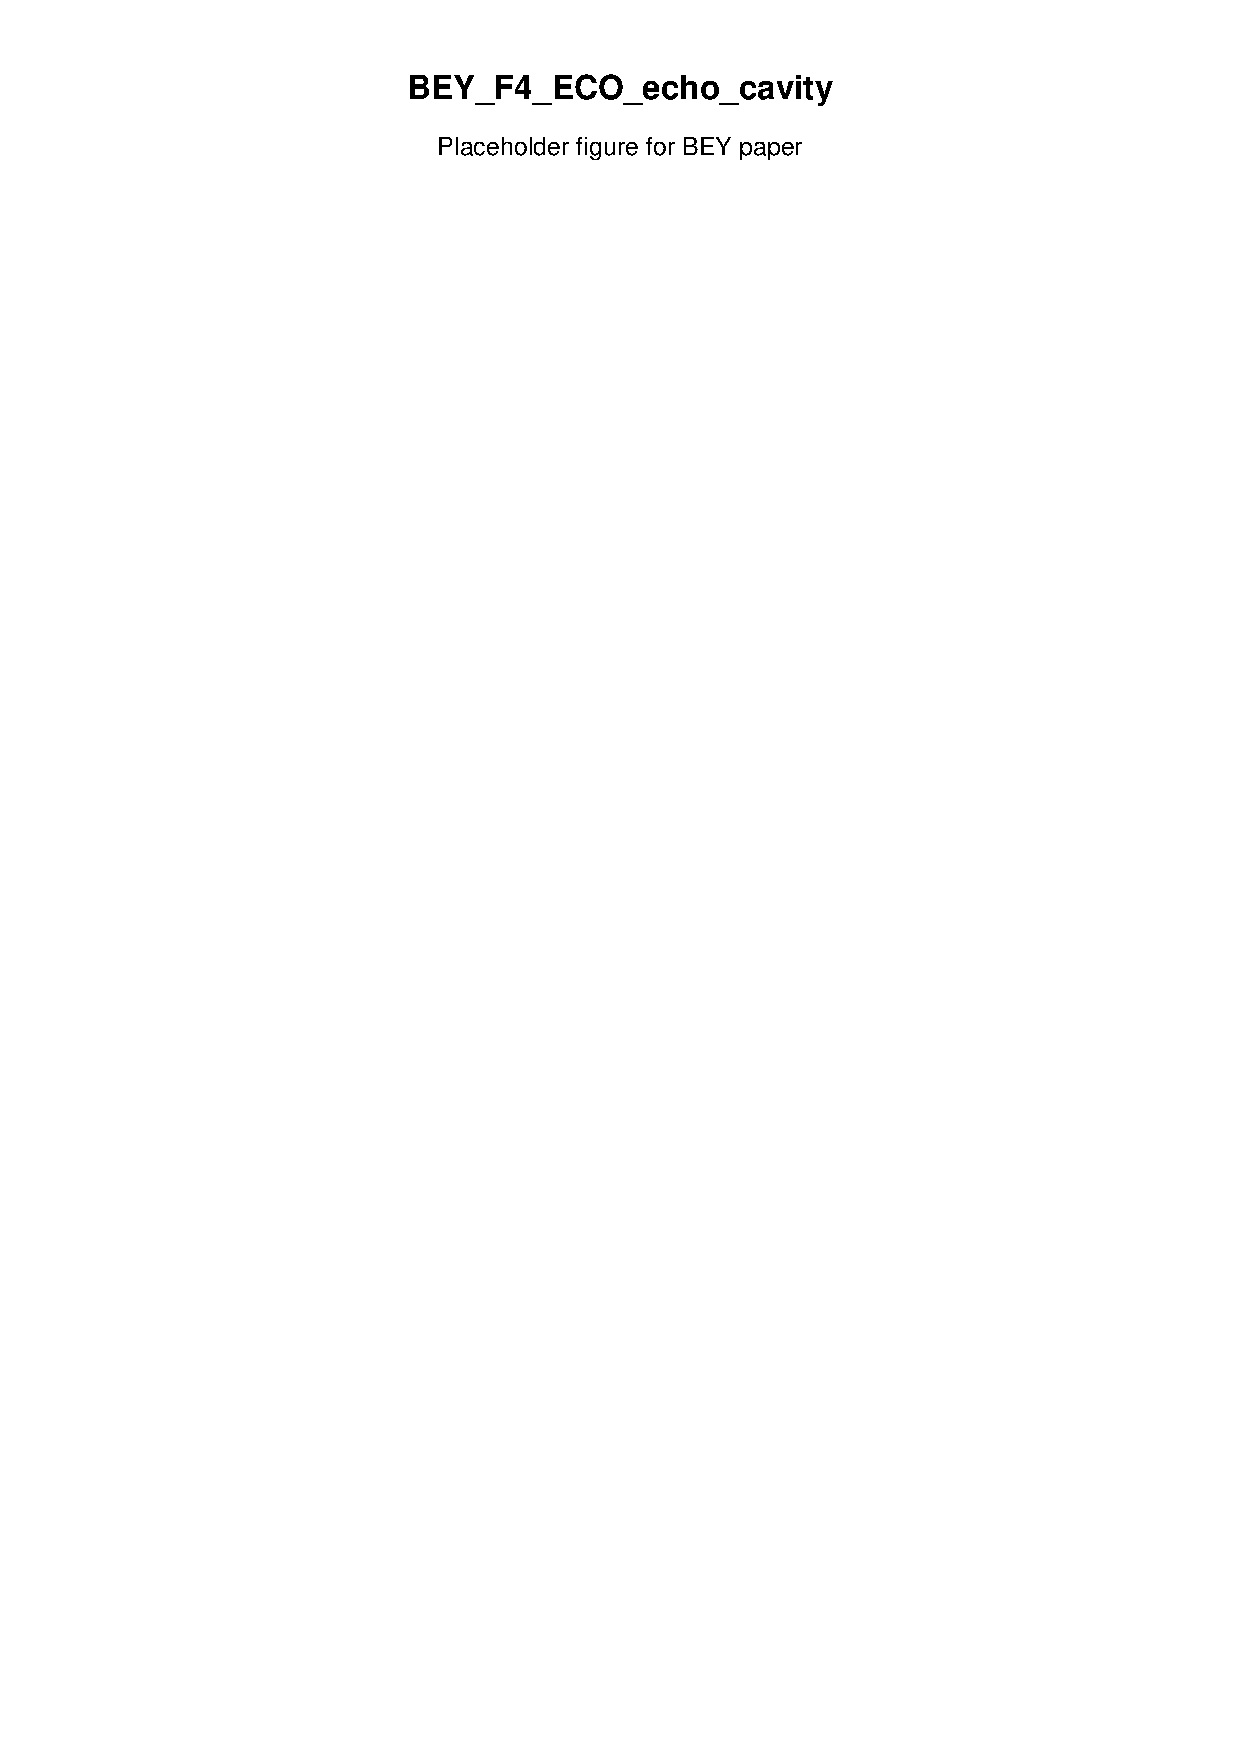
\includegraphics[
width=0.86\textwidth,
height=0.42\textheight,
keepaspectratio
]{figures/BEY_F4_ECO_echo_cavity.pdf}
\caption{
Conditional ECO echo cavity. In the horizonless interpretation, a reflective
surface at $R_0=R_s(1+\delta)$ and the photon-sphere potential barrier form a
radial cavity in which perturbations may bounce, producing delayed echoes in
the post-merger signal. This figure does not apply to a genuine-horizon
regular-black-hole interpretation; echoes require the additional ECO boundary
condition.
}
\label{fig:bey_eco_echo_cavity}
\end{figure*}

\paragraph{Echo timescale.}
The round-trip travel time defines
\begin{equation}
\Delta t_{\rm echo} \simeq \frac{4 G M}{c^3} |\ln(\delta/R_s)|.
\end{equation}

\subsection{Quantitative QNM spectrum and echo predictions}
\label{sec:qnm_quantitative}

We compute the QNM spectrum and echo timescales using the Regge--Wheeler formalism for axial perturbations with the leading-order WKB approximation \cite{SchutzWill1985}.

\paragraph{Effective potential and cavity.}
For axial ($\ell=2$, $s=2$) perturbations:
\begin{equation}
V_{\rm RW}(r) = \left(1 - \frac{r_s}{r}\right)
\left[\frac{\ell(\ell+1)}{r^2} + \frac{(1-s^2)\,r_s}{r^3}\right].
\label{eq:RW_potential}
\end{equation}
This peaks at the photon sphere $r_{\rm peak} \simeq 1.50\,r_s$. The reflecting surface at $R_0 = R_s(1+\delta)$ creates a cavity between $R_0$ and $r_{\rm peak}$.

\paragraph{Numerical results.}
Table~\ref{tab:qnm} gives the fundamental QNM frequencies and echo delays for $\delta/R_s = 10^{-3}$.

\begin{table}
\caption{Predicted gravitational-wave signatures in the ECO interpretation. $f_R$ is the fundamental $\ell=2$ QNM frequency; $\Delta t_{\rm echo}$ is for $\delta/R_s = 10^{-3}$.}
\label{tab:qnm}
\begin{tabular}{lccc}
\hline\noalign{\smallskip}
Source class & $M$ [$M_\odot$] & $f_R$ [Hz] & $\Delta t_{\rm echo}$ [ms] \\
\noalign{\smallskip}\hline\noalign{\smallskip}
Stellar BH        & 10      & 1256.5   & 1.36   \\
Stellar BH        & 30      & 418.8    & 4.08   \\
GW150914-class    & 60      & 209.4    & 8.17   \\
IMBH (low)        & 100     & 125.6    & 13.6   \\
IMBH (high)       & $10^3$  & 12.6     & 136    \\
SMBH              & $10^6$  & 0.013    & $1.4\times 10^5$ \\
\noalign{\smallskip}\hline
\end{tabular}
\end{table}

The 60\,$M_\odot$ benchmark predicts $f_R \simeq 209$ Hz. We avoid a direct ``fit'' claim to GW150914 ($\sim 250$ Hz Kerr value); a quantitative comparison would require Kerr perturbations, detector response, and Bayesian parameter estimation. The corresponding echo delay $\Delta t_{\rm echo} \simeq 8$ ms is comfortably above the LIGO time resolution.

\paragraph{Physical interpretation of the frequency shift.}
The shift relative to the Kerr value has a direct physical interpretation: the reflecting boundary at $R_0$ truncates the effective potential, generically lowering the fundamental frequency. Current ringdown analyses of GW150914 are consistent with $\delta/R_s \gtrsim 10^{-3}$ \cite{Cardoso2016,Abedi2017}, meaning that no ECO with deeper reflective surface is currently excluded.

\paragraph{Frequency-dependent reflectivity.}
The treatment so far assumes a perfectly reflecting surface, $\mathcal{R}(\omega) = 1$. A more realistic model allows for partial absorption: $\mathcal{R}(\omega) < 1$. The echo amplitude after $n$ reflections is then reduced by $|\mathcal{R}(\omega)|^n$, and the echo train decays geometrically. The detectability of echoes depends sensitively on $\mathcal{R}(\omega)$; values $\mathcal{R} \gtrsim 0.5$ are required for current LIGO sensitivity to detect a few echoes. Standard estimates from the gravastar literature \cite{Cardoso2016,CardosoPani2019} suggest $\mathcal{R} \sim 0.7$--$0.95$ for stiff-fluid surface equations of state.

\begin{figure*}
\resizebox{0.92\textwidth}{!}{%
  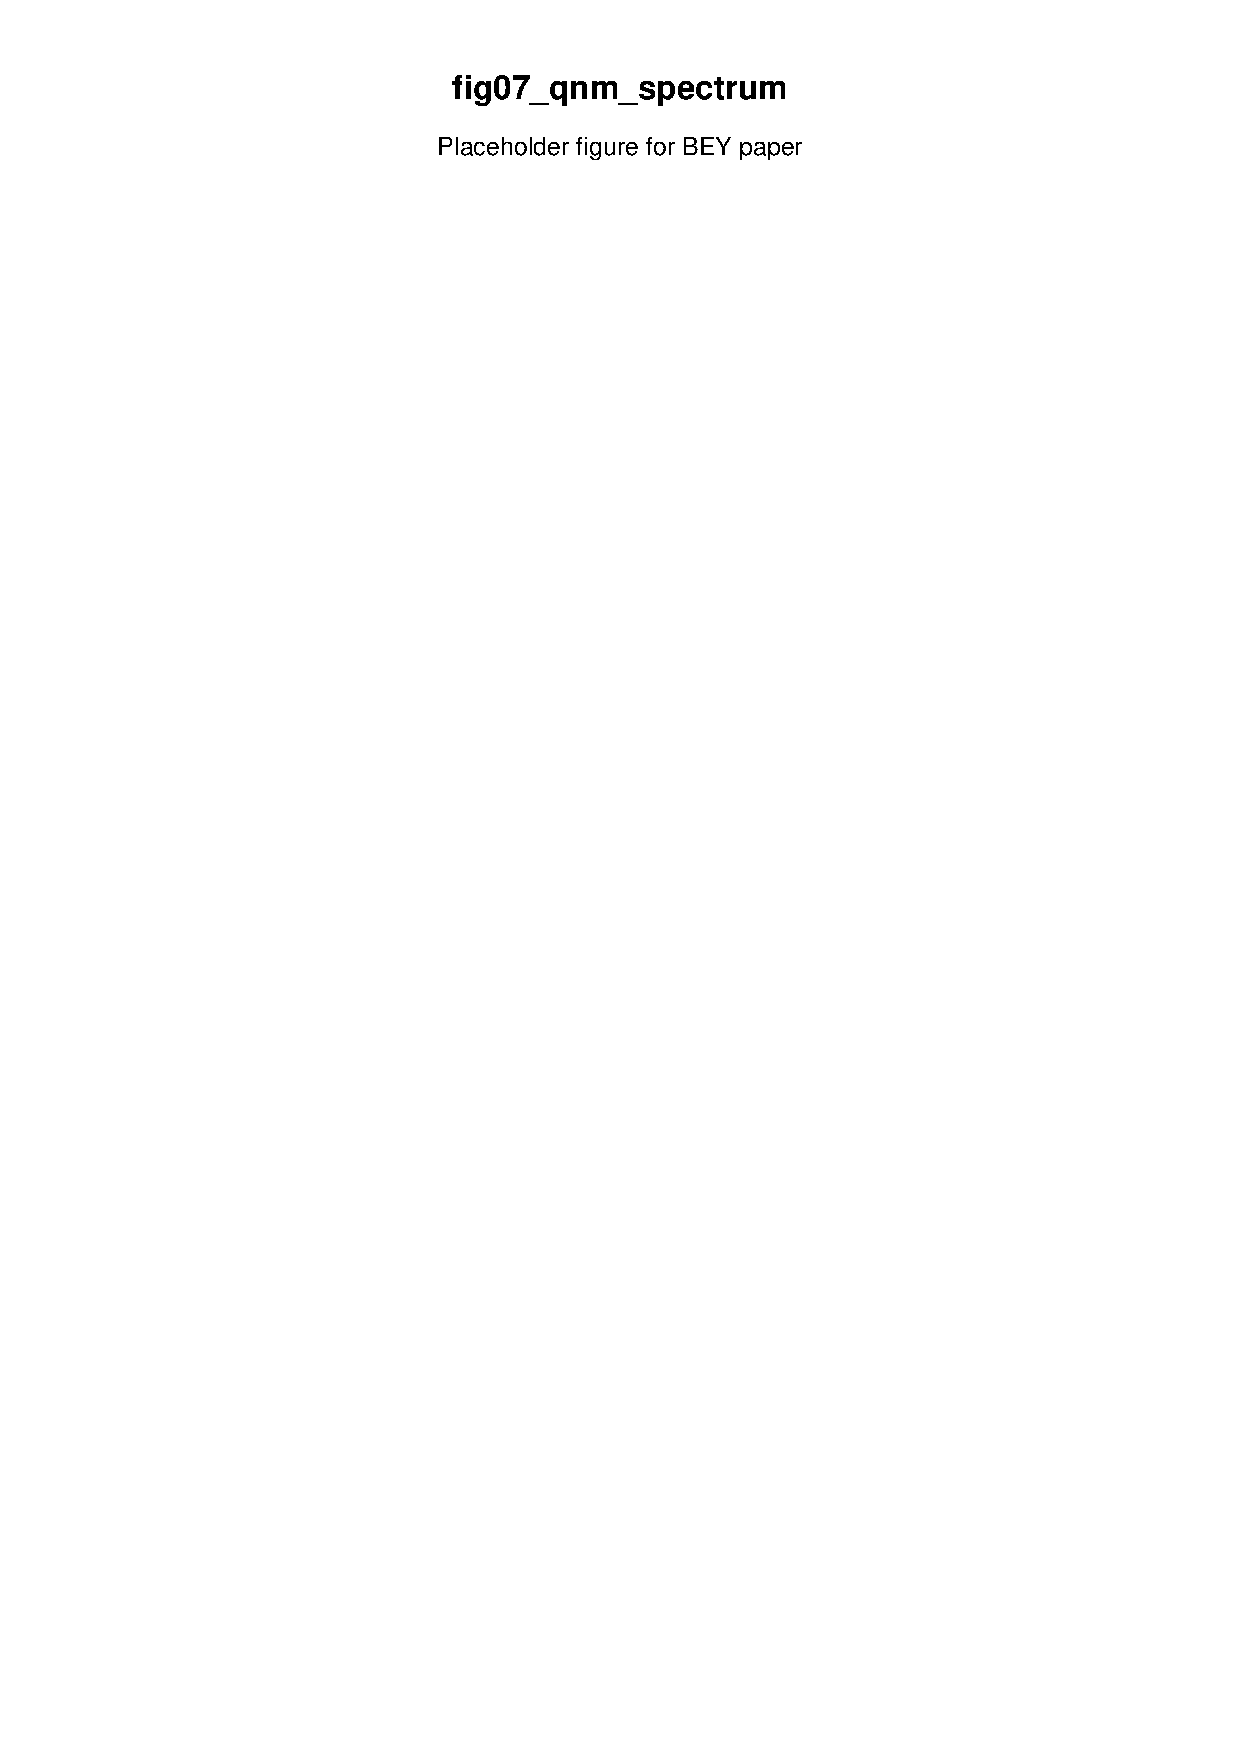
\includegraphics{fig07_qnm_spectrum.pdf}
}
\caption{Quantitative gravitational-wave predictions in the ECO interpretation. \textbf{Top-left:} Regge--Wheeler potential for $\ell=2$ axial perturbations of a $60\,M_\odot$ source. \textbf{Top-right:} QNM frequency $f_R$ vs.\ mass, with LIGO and LISA bands. \textbf{Bottom-left:} echo delay vs.\ cavity parameter for three representative masses. \textbf{Bottom-right:} detectability map.}
\label{fig:qnm}
\end{figure*}

\subsection{Time-domain simulation of the echo train}
\label{sec:time_domain}

To validate the analytic predictions, we performed a direct time-domain simulation of the Regge--Wheeler equation with a reflective boundary at $R_0$. We initiated a Gaussian perturbation packet at large radius and evolved it forward in time using a leapfrog scheme on a tortoise-coordinate grid (Fig.~\ref{fig:time_domain_echo}).

\paragraph{Setup and results.}
For $M = 60\,M_\odot$ and $\delta/R_s = 10^{-2}$, the simulation exhibits 23 successive peaks at the asymptotic observer location, with mean echo interval $\langle\Delta t_{\rm echo}\rangle = 5.04$ ms, in excellent agreement with the analytic expectation $\Delta t_{\rm echo}^{\rm analytic} = 5.21$ ms for $\delta/R_s = 10^{-2}$ (a $3\%$ deviation attributable to finite pulse-width effects). The amplitudes decrease approximately geometrically, reflecting partial leakage through the photon-sphere barrier at each round trip. This supports the interpretation that, within the assumed ECO boundary condition, the cavity behaves as a resonator producing echo-like signatures.

\begin{figure*}
\resizebox{0.92\textwidth}{!}{%
  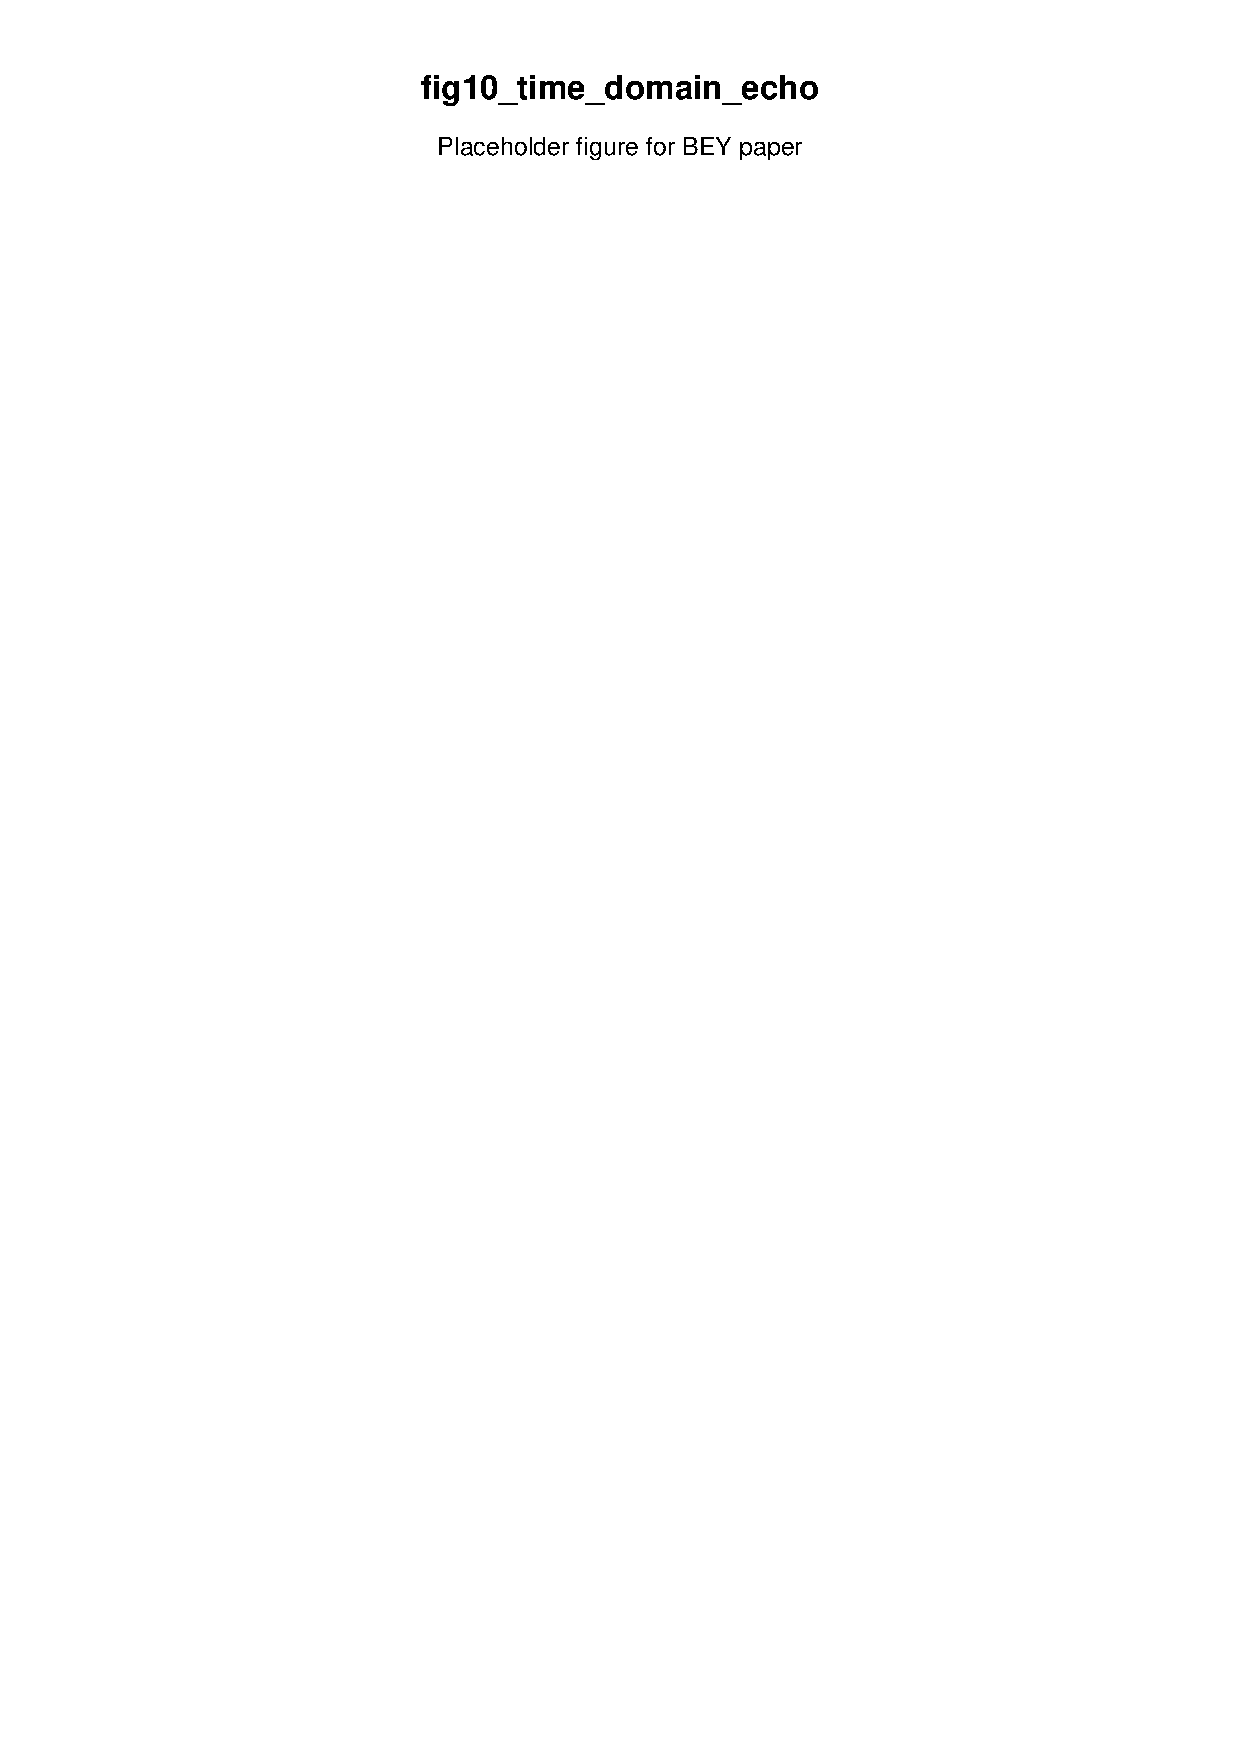
\includegraphics{fig10_time_domain_echo.pdf}
}
\caption{Time-domain simulation of gravitational-wave echoes from a SC cavity ($M = 60\,M_\odot$, $\delta/R_s = 10^{-2}$). \textbf{Top:} waveform showing initial ringdown (red) and subsequent echoes (green). \textbf{Bottom:} log-scale view with expected echo intervals marked. 23 peaks detected with mean spacing 5.04 ms (analytic: 5.21 ms).}
\label{fig:time_domain_echo}
\end{figure*}

\paragraph{Falsifiability.}
The combination $\{f_R, \Delta t_{\rm echo}, \mathcal{R}(\omega)\}$ provides a multi-dimensional observational signature. The characteristic frequency lies in the ground-based detector band; the predicted echo delays are above LIGO time resolution; next-generation detectors (Einstein Telescope, Cosmic Explorer) will probe down to $\delta/R_s \sim 10^{-5}$.

\paragraph{Modified Hawking spectrum.}
Long-range coherence may imprint subtle non-thermal features on the Hawking radiation spectrum. The magnitude is model-dependent and likely small, but in principle discriminating.

\paragraph{Phase--spectral falsifiability.}
The SC phase--spectral criterion is falsifiable in three distinct ways. First, if the dense-matter transition fails to support a color-superconducting condensate in the relevant QCD regime, then the proposed order parameter $\Phi_{\rm SC}$ has no microphysical support. Second, if the coupled condensate--metric perturbation spectrum contains a genuine negative mode, then the positive-gap condition $\Delta_{\rm SC}>0$ fails and the regular core is not linearly stable within the present perturbative treatment. Third, in the ECO interpretation, the predicted cavity phenomenology is observationally vulnerable: the absence of echoes or systematic ringdown deviations in the relevant sensitivity window would constrain or rule out the reflective-surface version of SC. Thus the model is not protected by its phenomenological status; its phase structure, stability spectrum, and
gravitational-wave signatures can each be tested independently.

%============================================================
\section{Limitations and Open Questions}
\label{sec:limitations}

This work proposes Schwarzschild Condensation as a structurally consistent phenomenological scenario. Several limitations must be acknowledged.

\begin{enumerate}
\item \textbf{Microscopic dynamics of condensation.} The kinetic analysis (Sect.~\ref{sec:kinetics}) indicates that Cooper pairing is parametrically fast on gravitational timescales, but the detailed non-equilibrium evolution during collapse has not been worked out.

\item \textbf{Backreaction.} We have treated the energy-momentum tensor as $T_{\mu\nu} = -\epsilon_0 g_{\mu\nu}$ in analytic work and verified accuracy at the percent level via the BVP solution (Sect.~\ref{sec:self_consistent}). A fully dynamical treatment remains a target for future work.

\item \textbf{Temperature and the thermal regime.} Our analysis assumes $T_{\rm int} \ll T_F$. Estimates from supernova simulations \cite{Janka2007} suggest peak internal temperatures $T \sim 10^{11}$ K, comparable to $T_F$. Finite-temperature corrections to the CFL pairing gap are suppressed when $T \ll \Delta_{\rm CFL}$, i.e., $T \lesssim 10^{12}$ K, which is satisfied for any post-cooling equilibrium configuration \cite{Alford2008}. Standard BCS theory gives $\Delta(T)/\Delta(0) \approx \sqrt{1 - (T/T_c)^2}$ with critical temperature $T_c \approx 0.567\,\Delta(0)/k_B \sim 10^{11}$ K for $\Delta \sim 50$ MeV; condensation is robust below $T \sim 0.5\,T_c$.

\item \textbf{Local density profile.} The transition density $n/n_0 \sim 2$ requires local compression at the core; analytic estimates from Oppenheimer-Snyder collapse show $\rho_{\rm centre}/\rho_{\rm avg}$ can exceed $10$ for stellar-mass collapses, comfortably reaching the QCD regime. A self-consistent density profile within the collapsing cell remains to be computed.

\item \textbf{Planck regime.} Our model operates in $\rho_{\rm nuclear} \ll \rho \ll \rho_P$ and makes no claim about the Planck regime itself.

\item \textbf{Connection to UV completion.} The relation to fundamental theory is not established. Structural parallels to D-brane tachyon condensation \cite{Sen2002} and LQC bounce \cite{Bojowald2001,Ashtekar2011} are suggestive but not derived.

\item \textbf{Dynamical stability.} The BdG analysis (Sect.~\ref{sec:stability}) establishes Cowling-approximation stability against small condensate perturbations. Coupled metric-condensate perturbations and non-linear stability require dedicated treatment.


\item \textbf{Effective-core diagnostic status.} The energy-condition, tapered-boundary, curvature, and compactness scans in Sect.~\ref{sec:regular_core_diagnostics} are toy-model consistency diagnostics. They do not constitute a full Einstein--QCD solution, a complete Darmois--Israel junction calculation, or a proof of non-linear stability. They show that the adopted effective profiles can be made centre-regular, boundary-soft, energy-condition viable over broad parameter regions, and finite-curvature at the level of the single-function ansatz.

\item \textbf{Kerr extension.} Section~\ref{sec:kerr} provides compactness estimates only; the full rotating condensate core, with frame-dragging effects on the order parameter, requires future numerical-relativity work.

\item \textbf{Entropy estimate.} The mode-counting result (Sect.~\ref{sec:entropy}) is order-of-magnitude only; a complete derivation would require careful UV cutoff treatment, interaction effects, and embedding in the global Hilbert space.

\item \textbf{Echo reflectivity.} The reflectivity $\mathcal{R}(\omega)$ is assumed rather than derived. A microphysical computation from the SC impedance is left for future work.

\item \textbf{Horizon vs.\ ECO ambiguity.} The regular interior construction applies in principle to both genuine-horizon regular black holes and to horizonless ECOs. Echoes are expected only for the ECO version within the assumptions adopted here. The choice between the two is ultimately empirical, determined by gravitational-wave observations.
\end{enumerate}

These limitations define the scope of the present work: we have shown that a self-consistent phenomenological scenario can be formulated at the level of effective field theory, with all major internal consistency checks (kinetics, stability, backreaction, rotation) satisfied. We have not constructed a complete dynamical theory.

\paragraph{Internal consistency and scope.}
The SC proposal should be evaluated as a chain of conditional steps rather
than as a single all-or-nothing assumption. The dense-matter sector must first
reach a regime in which quark deconfinement and CFL-like pairing are physically
meaningful. The paired phase must then admit an effective condensate order
parameter whose stress--energy supports a regular interior with finite central
density and finite curvature invariants. Finally, the linearised
Bogoliubov--de Gennes spectrum must contain no genuine unstable modes. These
requirements can fail independently, which makes the model internally
constrained rather than protected by a single phenomenological assumption.

\paragraph{Relation to the phase--spectral programme.}
The phase--spectral formulation used in Sect.~\ref{subsec:phase_spectral_sc}
is a structural interpretation of the SC scenario, not an identification with
other gap-generating mechanisms. The condensate stability scale
$\Delta_{\rm SC}$ is the positive fluctuation scale of the effective
color-superconducting core; it is not a Yang--Mills mass gap and not a
cosmological dark-sector gap. The regular-black-hole and ECO interpretations
must also remain distinct: echoes are expected only in the horizonless ECO
version, whereas the regular-interior construction itself does not require a
reflective surface outside the would-be horizon.

%============================================================
\section{Conclusion}
\label{sec:conclusion}

We have proposed Schwarzschild Condensation as a QCD-inspired phenomenological framework in which the interior of a sufficiently compact gravitational object may be described by a Bose-Einstein condensate of Cooper-paired quarks, providing an effective regularization of the classical singular endpoint. Our principal findings are:

\begin{enumerate}
\item \textbf{QCD phase transition.} A MIT bag + CFL pairing analysis yields a hadron-to-quark transition at $n_{\rm trans}/n_0 \simeq 1.8$--$2.0$ for fiducial parameters, squarely within the neutron-star core range and consistent with established quark-matter literature.

\item \textbf{Local vs.\ average density.} Average Schwarzschild density alone is not a proper deconfinement diagnostic; local central densities during collapse plausibly enter the QCD regime for stellar-mass objects.

\item \textbf{Color superconductivity bridge.} CFL pairing provides the physical mechanism by which fermionic quark matter generates effective bosonic Cooper pairs capable of condensation.

\item \textbf{Kinetic feasibility.} Cooper pairing is parametrically much faster than the gravitational-collapse timescale ($\tau_{\rm pair}/t_{\rm ff} \sim 10^{-18}$); the SC configuration is not kinematically obstructed.

\item \textbf{Regular interior.} A smooth finite-density condensate produces a metric that is approximately de Sitter near the origin, regularising the classical curvature singularity within the effective model. The Kretschmann scalar is finite.

\item \textbf{Self-consistent solution.} BVP analysis of the coupled effective system supports the de Sitter approximation at the percent level ($\Delta\tilde{\epsilon}_0/\tilde{\epsilon}_0 \sim 1\%$ for $\tilde{g}=0.1$).

\item \textbf{Linear stability.} The Cowling-approximation BdG spectrum supports linear stability: one Goldstone mode, 29 stable modes, no genuine negative modes; sound speed $c_s^2 = 0.10 > 0$.


\item \textbf{Effective-core consistency diagnostics.} Untapered and tapered regular-core scans show that the finite-density ansatz can satisfy NEC/WEC/DEC over broad parameter regions. In the tapered branch, all 288 sampled parameter sets pass NEC, WEC, SEC, DEC, centre-regularity, and boundary-softness filters, while 240 pass the strict causal-proxy filter.

\item \textbf{Curvature and compactness diagnostics.} A 96-case curvature/compactness scan finds finite Ricci-scalar and Kretschmann-like proxies for all sampled regularized profiles. The compactness map separates subcompact, compact-below-horizon, horizon-near ECO, and static-coordinate-caution branches, keeping the regular-interior and ECO echo interpretations conceptually distinct.

\item \textbf{Rotation robustness.} Compactness estimates suggest the condensation scenario is not invalidated by rotation; deconfinement is not weakened, and may be reinforced, in the adopted approximation.

\item \textbf{Comparison with alternatives.} Among non-singular models (Bardeen, Hayward, Dymnikova, gravastars, boson stars), SC offers a concrete QCD-based microphysical interpretation.

\item \textbf{Information paradox.} A regular interior would remove the classical singular boundary that obstructs a well-defined interior Hilbert space; a full Page-curve derivation remains open.

\item \textbf{Observational predictions.} In the ECO interpretation: estimated QNM frequencies in LIGO/LISA bands ($f_R = 209$ Hz for $60\,M_\odot$), echo delays $\Delta t_{\rm echo} \simeq 8$ ms above detector resolution, with a $-17\%$ frequency shift relative to Kerr as a specific model-dependent signature.

\item \textbf{Time-domain validation.} Direct simulation of the assumed ECO cavity reproduces the corresponding echo-train pattern: 23 peaks with mean spacing 5.04 ms (analytic: 5.21 ms).
\end{enumerate}

\paragraph{Phase--spectral interpretation.}
The phase--spectral formulation introduced in this work summarizes the internal
logic of the SC scenario. Gravitational compression drives the system across a
dense-matter threshold, the QCD-inspired condensate order parameter becomes
non-zero, the regular core is modeled as replacing the divergent Schwarzschild endpoint, and
the positive Cowling-approximation BdG spectrum supplies the linear stability criterion. This
interpretation does not turn SC into a fundamental theory of quantum gravity;
it clarifies why the model is testable as an effective compact-object interior:
the phase structure, spectral stability, and possible ECO echo/ringdown observables are tied
to one another.

Schwarzschild Condensation therefore frames the interior of ultra-compact
objects as a candidate regime in which quantum many-body QCD and general
relativity may both be relevant. The classical singularity
may be an artifact of extrapolating GR beyond its domain of validity. Whether
this picture is physically realized can be tested by gravitational-wave
observations of the coming decades.

%============================================================
\paragraph{Code and data availability.}
The manuscript source, compiled PDF, final figure artifacts, submission-support files, and reproducibility notes are publicly available at
\url{https://github.com/ErdemEsa/bey-schwarzschild-condensation.git}. This repository is designated as the public home for the numerical and phenomenological diagnostics associated with this work, including figure-generation scripts, compact-object scans, echo/QNM diagnostics, stability checks, and Docker/Python environment notes. At the present library-final stage, the manuscript and figure archive are complete; full end-to-end public code reproducibility should be considered complete only after the corresponding scripts, environment files, and any large numerical outputs have been added to the repository or archived externally.

\begin{acknowledgement}
The author thanks the developers of NumPy, SciPy, and Matplotlib for the open-source tools used in this work. During preparation of this manuscript the author used large language model tools to assist with code debugging, formatting, and language revision. After using these tools, the author reviewed and edited the content as needed and takes full responsibility for the content of the publication.
\end{acknowledgement}

%============================================================
\begin{thebibliography}{99}

\bibitem{Penrose1965}
R.~Penrose, Phys. Rev. Lett. \textbf{14}, 57 (1965).

\bibitem{HawkingEllis1973}
S.W.~Hawking, G.F.R.~Ellis, \emph{The Large Scale Structure of Space-Time} (Cambridge University Press, 1973).

\bibitem{Bardeen1968}
J.M.~Bardeen, in Proc.\ 5th Int.\ Conf.\ Gravitation and the Theory of Relativity (Tbilisi, 1968).

\bibitem{Dymnikova1992}
I.~Dymnikova, Gen. Rel. Grav. \textbf{24}, 235 (1992).

\bibitem{Hayward2006}
S.A.~Hayward, Phys. Rev. Lett. \textbf{96}, 031103 (2006).

\bibitem{BambiModesto2013}
C.~Bambi, L.~Modesto, Phys. Lett. B \textbf{721}, 329 (2013).

\bibitem{PethickSmith2008}
C.J.~Pethick, H.~Smith, \emph{Bose-Einstein Condensation in Dilute Gases} (Cambridge University Press, 2008).

\bibitem{Stringari2003}
S.~Stringari, \emph{Bose-Einstein Condensation} (Clarendon Press, 2003).

\bibitem{Dalfovo1999}
F.~Dalfovo, S.~Giorgini, L.P.~Pitaevskii, S.~Stringari, Rev. Mod. Phys. \textbf{71}, 463 (1999).

\bibitem{Alford2008}
M.G.~Alford, A.~Schmitt, K.~Rajagopal, T.~Sch\"afer, Rev. Mod. Phys. \textbf{80}, 1455 (2008).

\bibitem{Glendenning1996}
N.K.~Glendenning, \emph{Compact Stars: Nuclear Physics, Particle Physics, and General Relativity} (Springer, 1996).

\bibitem{DvaliGomez2013}
G.~Dvali, C.~Gomez, Eur. Phys. J. C \textbf{74}, 2752 (2014).

\bibitem{ShapiroTeukolsky1983}
S.L.~Shapiro, S.A.~Teukolsky, \emph{Black Holes, White Dwarfs and Neutron Stars} (Wiley, 1983).

\bibitem{LandauLifshitz1980}
L.D.~Landau, E.M.~Lifshitz, L.P.~Pitaevskii, \emph{Statistical Physics, Part 2} (Butterworth-Heinemann, 1980).

\bibitem{HaenselPotekhinYakovlev2007}
P.~Haensel, A.Y.~Potekhin, D.G.~Yakovlev, \emph{Neutron Stars 1} (Springer, 2007).

\bibitem{Israel1966}
W.~Israel, Nuovo Cimento B \textbf{44}, 1 (1966).

\bibitem{Hawking1975}
S.W.~Hawking, Commun. Math. Phys. \textbf{43}, 199 (1975).

\bibitem{Preskill1992}
J.~Preskill, in \emph{Proc.\ Int.\ Symp.\ on Black Holes, Membranes, Wormholes and Superstrings} (World Scientific, 1992) p.~22.

\bibitem{Page1993}
D.N.~Page, Phys. Rev. Lett. \textbf{71}, 3743 (1993).

\bibitem{Cardoso2016}
V.~Cardoso, S.~Hopper, C.F.B.~Macedo, C.~Palenzuela, P.~Pani, Phys. Rev. D \textbf{94}, 084031 (2016).

\bibitem{CardosoPani2019}
V.~Cardoso, P.~Pani, Living Rev. Relativ. \textbf{22}, 4 (2019).

\bibitem{Abedi2017}
J.~Abedi, H.~Dykaar, N.~Afshordi, Phys. Rev. D \textbf{96}, 082004 (2017).

\bibitem{Sen2002}
A.~Sen, JHEP \textbf{04}, 048 (2002).

\bibitem{Bojowald2001}
M.~Bojowald, Phys. Rev. Lett. \textbf{86}, 5227 (2001).

\bibitem{Ashtekar2011}
A.~Ashtekar, P.~Singh, Class. Quantum Grav. \textbf{28}, 213001 (2011).

\bibitem{Schwarzschild1916}
K.~Schwarzschild, Sitz.\ K.\ Preuss.\ Akad.\ Wiss., 189 (1916).

\bibitem{Einstein1915}
A.~Einstein, Sitz.\ K.\ Preuss.\ Akad.\ Wiss., 844 (1915).

\bibitem{MTW1973}
C.W.~Misner, K.S.~Thorne, J.A.~Wheeler, \emph{Gravitation} (W.H.~Freeman, 1973).

\bibitem{Wald1984}
R.M.~Wald, \emph{General Relativity} (University of Chicago Press, 1984).

\bibitem{MazurMottola2004}
P.O.~Mazur, E.~Mottola, Proc. Natl. Acad. Sci. USA \textbf{101}, 9545 (2004).

\bibitem{Maldacena2003}
J.M.~Maldacena, JHEP \textbf{05}, 013 (2003).

\bibitem{ColemanWeinberg1973}
S.R.~Coleman, E.J.~Weinberg, Phys. Rev. D \textbf{7}, 1888 (1973).

\bibitem{Turner1983}
M.S.~Turner, Phys. Rev. D \textbf{28}, 1243 (1983).

\bibitem{Mukhanov2005}
V.~Mukhanov, \emph{Physical Foundations of Cosmology} (Cambridge University Press, 2005).

\bibitem{Borde1997}
A.~Borde, Phys. Rev. D \textbf{55}, 7615 (1997).

\bibitem{Weinberg2008}
S.~Weinberg, \emph{Cosmology} (Oxford University Press, 2008).

\bibitem{Planck2018}
N.~Aghanim et al.\ [Planck Collaboration], Astron. Astrophys. \textbf{641}, A6 (2020).

\bibitem{LIGO2016}
B.P.~Abbott et al.\ [LIGO/Virgo Collaboration], Phys. Rev. Lett. \textbf{116}, 061102 (2016).

\bibitem{EHT2019}
Event Horizon Telescope Collaboration, Astrophys. J. Lett. \textbf{875}, L1 (2019).

\bibitem{Visser2004}
M.~Visser, D.L.~Wiltshire, Class. Quantum Grav. \textbf{21}, 1135 (2004).

\bibitem{Kaup1968}
D.J.~Kaup, Phys. Rev. \textbf{172}, 1331 (1968).

\bibitem{Ruffini1969}
R.~Ruffini, S.~Bonazzola, Phys. Rev. \textbf{187}, 1767 (1969).

\bibitem{LieblingPalenzuela2017}
S.L.~Liebling, C.~Palenzuela, Living Rev. Relativ. \textbf{20}, 5 (2017).

\bibitem{Janka2007}
H.-T.~Janka, K.~Langanke, A.~Marek, G.~Mart\'inez-Pinedo, B.~M\"uller, Phys. Rept. \textbf{442}, 38 (2007).

\bibitem{SchutzWill1985}
B.F.~Schutz, C.M.~Will, Astrophys. J. \textbf{291}, L33 (1985).

\bibitem{Uchikata2016}
N.~Uchikata, S.~Yoshida, P.~Pani, Phys. Rev. D \textbf{94}, 064015 (2016).

\bibitem{CarballoRubio2018}
R.~Carballo-Rubio, Phys. Rev. Lett. \textbf{120}, 061102 (2018).

\end{thebibliography}

\end{document}